\documentclass[twoside]{book}

% Packages required by doxygen
\usepackage{fixltx2e}
\usepackage{calc}
\usepackage{doxygen}
\usepackage[export]{adjustbox} % also loads graphicx
\usepackage{graphicx}
\usepackage[utf8]{inputenc}
\usepackage{makeidx}
\usepackage{multicol}
\usepackage{multirow}
\PassOptionsToPackage{warn}{textcomp}
\usepackage{textcomp}
\usepackage[nointegrals]{wasysym}
\usepackage[table]{xcolor}

% Font selection
\usepackage[T1]{fontenc}
\usepackage[scaled=.90]{helvet}
\usepackage{courier}
\usepackage{amssymb}
\usepackage{sectsty}
\renewcommand{\familydefault}{\sfdefault}
\allsectionsfont{%
  \fontseries{bc}\selectfont%
  \color{darkgray}%
}
\renewcommand{\DoxyLabelFont}{%
  \fontseries{bc}\selectfont%
  \color{darkgray}%
}
\newcommand{\+}{\discretionary{\mbox{\scriptsize$\hookleftarrow$}}{}{}}

% Page & text layout
\usepackage{geometry}
\geometry{%
  a4paper,%
  top=2.5cm,%
  bottom=2.5cm,%
  left=2.5cm,%
  right=2.5cm%
}
\tolerance=750
\hfuzz=15pt
\hbadness=750
\setlength{\emergencystretch}{15pt}
\setlength{\parindent}{0cm}
\setlength{\parskip}{3ex plus 2ex minus 2ex}
\makeatletter
\renewcommand{\paragraph}{%
  \@startsection{paragraph}{4}{0ex}{-1.0ex}{1.0ex}{%
    \normalfont\normalsize\bfseries\SS@parafont%
  }%
}
\renewcommand{\subparagraph}{%
  \@startsection{subparagraph}{5}{0ex}{-1.0ex}{1.0ex}{%
    \normalfont\normalsize\bfseries\SS@subparafont%
  }%
}
\makeatother

% Headers & footers
\usepackage{fancyhdr}
\pagestyle{fancyplain}
\fancyhead[LE]{\fancyplain{}{\bfseries\thepage}}
\fancyhead[CE]{\fancyplain{}{}}
\fancyhead[RE]{\fancyplain{}{\bfseries\leftmark}}
\fancyhead[LO]{\fancyplain{}{\bfseries\rightmark}}
\fancyhead[CO]{\fancyplain{}{}}
\fancyhead[RO]{\fancyplain{}{\bfseries\thepage}}
\fancyfoot[LE]{\fancyplain{}{}}
\fancyfoot[CE]{\fancyplain{}{}}
\fancyfoot[RE]{\fancyplain{}{\bfseries\scriptsize Generated by Doxygen }}
\fancyfoot[LO]{\fancyplain{}{\bfseries\scriptsize Generated by Doxygen }}
\fancyfoot[CO]{\fancyplain{}{}}
\fancyfoot[RO]{\fancyplain{}{}}
\renewcommand{\footrulewidth}{0.4pt}
\renewcommand{\chaptermark}[1]{%
  \markboth{#1}{}%
}
\renewcommand{\sectionmark}[1]{%
  \markright{\thesection\ #1}%
}

% Indices & bibliography
\usepackage{natbib}
\usepackage[titles]{tocloft}
\setcounter{tocdepth}{3}
\setcounter{secnumdepth}{5}
\makeindex

% Hyperlinks (required, but should be loaded last)
\usepackage{ifpdf}
\ifpdf
  \usepackage[pdftex,pagebackref=true]{hyperref}
\else
  \usepackage[ps2pdf,pagebackref=true]{hyperref}
\fi
\hypersetup{%
  colorlinks=true,%
  linkcolor=blue,%
  citecolor=blue,%
  unicode%
}

% Custom commands
\newcommand{\clearemptydoublepage}{%
  \newpage{\pagestyle{empty}\cleardoublepage}%
}

\usepackage{caption}
\captionsetup{labelsep=space,justification=centering,font={bf},singlelinecheck=off,skip=4pt,position=top}

%===== C O N T E N T S =====

\begin{document}

% Titlepage & ToC
\hypersetup{pageanchor=false,
             bookmarksnumbered=true,
             pdfencoding=unicode
            }
\pagenumbering{roman}
\begin{titlepage}
\vspace*{7cm}
\begin{center}%
{\Large My Project }\\
\vspace*{1cm}
{\large Generated by Doxygen 1.8.11}\\
\end{center}
\end{titlepage}
\clearemptydoublepage
\tableofcontents
\clearemptydoublepage
\pagenumbering{arabic}
\hypersetup{pageanchor=true}

%--- Begin generated contents ---
\chapter{Bug List}
\label{bug}
\hypertarget{bug}{}

\begin{DoxyRefList}
\item[\label{bug__bug000002}%
\hypertarget{bug__bug000002}{}%
Class \hyperlink{classdelaunay3}{delaunay3} ]No known bugs.  
\item[\label{bug__bug000001}%
\hypertarget{bug__bug000001}{}%
File \hyperlink{delaunay3_8h}{delaunay3.h} ]No known bugs. 

No known bugs.  
\item[\label{bug__bug000004}%
\hypertarget{bug__bug000004}{}%
Class \hyperlink{classdijkstraPQ}{dijkstra\+PQ} ]No known bugs.  
\item[\label{bug__bug000027}%
\hypertarget{bug__bug000027}{}%
File \hyperlink{dijkstraPQ_8cpp}{dijkstra\+PQ.cpp} ]No known bugs.  
\item[\label{bug__bug000003}%
\hypertarget{bug__bug000003}{}%
File \hyperlink{dijkstraPQ_8h}{dijkstra\+PQ.h} ]No known bugs.  
\item[\label{bug__bug000006}%
\hypertarget{bug__bug000006}{}%
Class \hyperlink{classfindNearestPoint}{find\+Nearest\+Point} ]No known bugs.  
\item[\label{bug__bug000005}%
\hypertarget{bug__bug000005}{}%
File \hyperlink{findNearestPoint_8cpp}{find\+Nearest\+Point.cpp} ]No known bugs. 

No known bugs.  
\item[\label{bug__bug000023}%
\hypertarget{bug__bug000023}{}%
File \hyperlink{jointControlKuka_8cpp}{joint\+Control\+Kuka.cpp} ]No known bugs.  
\item[\label{bug__bug000008}%
\hypertarget{bug__bug000008}{}%
Class \hyperlink{classkukaControl}{kuka\+Control} ]No known bugs.  
\item[\label{bug__bug000025}%
\hypertarget{bug__bug000025}{}%
File \hyperlink{kukaControl_8cpp}{kuka\+Control.cpp} ]No known bugs.  
\item[\label{bug__bug000007}%
\hypertarget{bug__bug000007}{}%
File \hyperlink{kukaControl_8h}{kuka\+Control.h} ]No known bugs.  
\item[\label{bug__bug000037}%
\hypertarget{bug__bug000037}{}%
File \hyperlink{main_8cpp}{main.cpp} ]No known bugs.  
\item[\label{bug__bug000010}%
\hypertarget{bug__bug000010}{}%
Class \hyperlink{classpclCloudViewer}{pcl\+Cloud\+Viewer} ]No known bugs.  
\item[\label{bug__bug000029}%
\hypertarget{bug__bug000029}{}%
File \hyperlink{pclCloudViewer_8cpp}{pcl\+Cloud\+Viewer.cpp} ]No known bugs. 

No1 can\textquotesingle{}t not be compile successfully in the test case.  
\item[\label{bug__bug000009}%
\hypertarget{bug__bug000009}{}%
File \hyperlink{pclCloudViewer_8h}{pcl\+Cloud\+Viewer.h} ]No1 can\textquotesingle{}t not be compile successfully in the test case.  
\item[\label{bug__bug000012}%
\hypertarget{bug__bug000012}{}%
Class \hyperlink{classpclFastTriangular}{pcl\+Fast\+Triangular} ]No known bugs.  
\item[\label{bug__bug000031}%
\hypertarget{bug__bug000031}{}%
File \hyperlink{pclFastTriangular_8cpp}{pcl\+Fast\+Triangular.cpp} ]No known bugs.  
\item[\label{bug__bug000011}%
\hypertarget{bug__bug000011}{}%
File \hyperlink{pclFastTriangular_8h}{pcl\+Fast\+Triangular.h} ]No known bugs.  
\item[\label{bug__bug000038}%
\hypertarget{bug__bug000038}{}%
File \hyperlink{pclFastTriangularTest_8cpp}{pcl\+Fast\+Triangular\+Test.cpp} ]No known bugs.  
\item[\label{bug__bug000014}%
\hypertarget{bug__bug000014}{}%
Class \hyperlink{classpclIo}{pcl\+Io} ]No known bugs.  
\item[\label{bug__bug000032}%
\hypertarget{bug__bug000032}{}%
File \hyperlink{pclIo_8cpp}{pcl\+Io.cpp} ]No known bugs.  
\item[\label{bug__bug000013}%
\hypertarget{bug__bug000013}{}%
File \hyperlink{pclIo_8h}{pcl\+Io.h} ]No known bugs.  
\item[\label{bug__bug000039}%
\hypertarget{bug__bug000039}{}%
File \hyperlink{pclIoTest_8cpp}{pcl\+Io\+Test.cpp} ]No known bugs.  
\item[\label{bug__bug000016}%
\hypertarget{bug__bug000016}{}%
Class \hyperlink{classpclMlsSmoothing}{pcl\+Mls\+Smoothing} ]No known bugs.  
\item[\label{bug__bug000033}%
\hypertarget{bug__bug000033}{}%
File \hyperlink{pclMlsSmoothing_8cpp}{pcl\+Mls\+Smoothing.cpp} ]No known bugs.  
\item[\label{bug__bug000015}%
\hypertarget{bug__bug000015}{}%
File \hyperlink{pclMlsSmoothing_8h}{pcl\+Mls\+Smoothing.h} ]No known bugs.  
\item[\label{bug__bug000040}%
\hypertarget{bug__bug000040}{}%
File \hyperlink{pclMlsSmoothingTest_8cpp}{pcl\+Mls\+Smoothing\+Test.cpp} ]No known bugs.  
\item[\label{bug__bug000018}%
\hypertarget{bug__bug000018}{}%
Class \hyperlink{classpclPassThrough}{pcl\+Pass\+Through} ]No known bugs.  
\item[\label{bug__bug000034}%
\hypertarget{bug__bug000034}{}%
File \hyperlink{pclPassThrough_8cpp}{pcl\+Pass\+Through.cpp} ]No known bugs.  
\item[\label{bug__bug000041}%
\hypertarget{bug__bug000041}{}%
File \hyperlink{pclPassThroughTest_8cpp}{pcl\+Pass\+Through\+Test.cpp} ]No known bugs.  
\item[\label{bug__bug000035}%
\hypertarget{bug__bug000035}{}%
File \hyperlink{pclStatisticalOutlierRemoval_8cpp}{pcl\+Statistical\+Outlier\+Removal.cpp} ]No known bugs.  
\item[\label{bug__bug000042}%
\hypertarget{bug__bug000042}{}%
File \hyperlink{pclStatisticalOutlierRemovalTest_8cpp}{pcl\+Statistical\+Outlier\+Removal\+Test.cpp} ]No known bugs.  
\item[\label{bug__bug000020}%
\hypertarget{bug__bug000020}{}%
Class \hyperlink{classpclStatistOutRev}{pcl\+Statist\+Out\+Rev} ]No known bugs.  
\item[\label{bug__bug000022}%
\hypertarget{bug__bug000022}{}%
Class \hyperlink{classpclVoxel}{pcl\+Voxel} ]No known bugs.  
\item[\label{bug__bug000036}%
\hypertarget{bug__bug000036}{}%
File \hyperlink{pclVoxel_8cpp}{pcl\+Voxel.cpp} ]No known bugs.  
\item[\label{bug__bug000021}%
\hypertarget{bug__bug000021}{}%
File \hyperlink{pclVoxel_8h}{pcl\+Voxel.h} ]No known bugs.  
\item[\label{bug__bug000043}%
\hypertarget{bug__bug000043}{}%
File \hyperlink{pclVoxelTest_8cpp}{pcl\+Voxel\+Test.cpp} ]No known bugs.  
\item[\label{bug__bug000024}%
\hypertarget{bug__bug000024}{}%
File \hyperlink{talker_8cpp}{talker.cpp} ]No known bugs. 
\end{DoxyRefList}
\chapter{Class Index}
\section{Class List}
Here are the classes, structs, unions and interfaces with brief descriptions\+:\begin{DoxyCompactList}
\item\contentsline{section}{\hyperlink{classdelaunay3}{delaunay3} \\*This \hyperlink{delaunay3_8h}{delaunay3.\+h} is a header file of the meshing triangle among the point cloud }{\pageref{classdelaunay3}}{}
\item\contentsline{section}{\hyperlink{classdijkstraPQ}{dijkstra\+PQ} \\*Kuka\+Control is a header file of finding shortest path among the point cloud }{\pageref{classdijkstraPQ}}{}
\item\contentsline{section}{\hyperlink{structDupex}{Dupex} }{\pageref{structDupex}}{}
\item\contentsline{section}{\hyperlink{classfindNearestPoint}{find\+Nearest\+Point} \\*Find\+Nearest\+Point is an finding the closest point on a post smoothing surface }{\pageref{classfindNearestPoint}}{}
\item\contentsline{section}{\hyperlink{classkukaControl}{kuka\+Control} \\*Kuka\+Control is an implementation of controlling the iiwa kuka arm
\begin{DoxyItemize}
\item 
\end{DoxyItemize}}{\pageref{classkukaControl}}{}
\item\contentsline{section}{\hyperlink{classpclCloudViewer}{pcl\+Cloud\+Viewer} \\*Pcl\+Cloud\+Viewer is an implementation by using pcl visualization to display the point cloud
\begin{DoxyItemize}
\item 
\end{DoxyItemize}}{\pageref{classpclCloudViewer}}{}
\item\contentsline{section}{\hyperlink{classpclFastTriangular}{pcl\+Fast\+Triangular} \\*Pcl\+Fast\+Triangular is an implementation by using pcl fast\+Triangular method to reconstruct the surface.
\begin{DoxyItemize}
\item 
\end{DoxyItemize}}{\pageref{classpclFastTriangular}}{}
\item\contentsline{section}{\hyperlink{classpclIo}{pcl\+Io} \\*Pcl\+Io is an implementation by using pcl to load .pcd file from local.
\begin{DoxyItemize}
\item 
\end{DoxyItemize}}{\pageref{classpclIo}}{}
\item\contentsline{section}{\hyperlink{classpclMlsSmoothing}{pcl\+Mls\+Smoothing} \\*Pcl\+Mls\+Smoothing is an implementation by using moving least square(mls) method to smooth the point cloud among the surface }{\pageref{classpclMlsSmoothing}}{}
\item\contentsline{section}{\hyperlink{classpclPassThrough}{pcl\+Pass\+Through} \\*Pcl\+Pass\+Through is an implementation by using pcl passthrough filter to extract certain region of point cloud.
\begin{DoxyItemize}
\item 
\end{DoxyItemize}}{\pageref{classpclPassThrough}}{}
\item\contentsline{section}{\hyperlink{classpclStatistOutRev}{pcl\+Statist\+Out\+Rev} \\*Pcl\+Statist\+Out\+Rev is an implementation by using pcl pcl\+Statist\+Outlier\+Removal filter to filter noise in point cloud
\begin{DoxyItemize}
\item 
\end{DoxyItemize}}{\pageref{classpclStatistOutRev}}{}
\item\contentsline{section}{\hyperlink{classpclVoxel}{pcl\+Voxel} \\*Pcl\+Voxel is an implementation by using pcl voxel\+\_\+grid filter to down sample the point cloud
\begin{DoxyItemize}
\item 
\end{DoxyItemize}}{\pageref{classpclVoxel}}{}
\item\contentsline{section}{\hyperlink{structposition}{position} }{\pageref{structposition}}{}
\item\contentsline{section}{\hyperlink{structShx}{Shx} }{\pageref{structShx}}{}
\item\contentsline{section}{\hyperlink{structTriad}{Triad} }{\pageref{structTriad}}{}
\end{DoxyCompactList}

\chapter{File Index}
\section{File List}
Here is a list of all documented files with brief descriptions\+:\begin{DoxyCompactList}
\item\contentsline{section}{/home/viki/catkin\+\_\+ws/src/\+Robotic-\/polishing/include/\hyperlink{delaunay3_8h}{delaunay3.\+h} \\*This \hyperlink{delaunay3_8h}{delaunay3.\+h} is a header file of the meshing triangle among the point cloud }{\pageref{delaunay3_8h}}{}
\item\contentsline{section}{/home/viki/catkin\+\_\+ws/src/\+Robotic-\/polishing/include/\hyperlink{dijkstraPQ_8h}{dijkstra\+P\+Q.\+h} \\*This \hyperlink{dijkstraPQ_8cpp}{dijkstra\+P\+Q.\+cpp} is a header file of finding shortest path among the point cloud. The algorithm refer to here\+: \href{http://www.geeksforgeeks.org/dijkstras-shortest-path-algorithm-using-priority_queue-stl/}{\tt http\+://www.\+geeksforgeeks.\+org/dijkstras-\/shortest-\/path-\/algorithm-\/using-\/priority\+\_\+queue-\/stl/} }{\pageref{dijkstraPQ_8h}}{}
\item\contentsline{section}{/home/viki/catkin\+\_\+ws/src/\+Robotic-\/polishing/include/{\bfseries find\+Nearest\+Point.\+h} }{\pageref{findNearestPoint_8h}}{}
\item\contentsline{section}{/home/viki/catkin\+\_\+ws/src/\+Robotic-\/polishing/include/\hyperlink{kukaControl_8h}{kuka\+Control.\+h} \\*This \hyperlink{kukaControl_8h}{kuka\+Control.\+h} is a header file of controlling the iiwa kuka arm }{\pageref{kukaControl_8h}}{}
\item\contentsline{section}{/home/viki/catkin\+\_\+ws/src/\+Robotic-\/polishing/include/\hyperlink{pclCloudViewer_8h}{pcl\+Cloud\+Viewer.\+h} \\*Header file of an \hyperlink{classpclCloudViewer}{pcl\+Cloud\+Viewer} class }{\pageref{pclCloudViewer_8h}}{}
\item\contentsline{section}{/home/viki/catkin\+\_\+ws/src/\+Robotic-\/polishing/include/\hyperlink{pclFastTriangular_8h}{pcl\+Fast\+Triangular.\+h} \\*Header file of an \hyperlink{classpclFastTriangular}{pcl\+Fast\+Triangular} class }{\pageref{pclFastTriangular_8h}}{}
\item\contentsline{section}{/home/viki/catkin\+\_\+ws/src/\+Robotic-\/polishing/include/\hyperlink{pclIo_8h}{pcl\+Io.\+h} \\*Header file of an \hyperlink{classpclIo}{pcl\+Io} class }{\pageref{pclIo_8h}}{}
\item\contentsline{section}{/home/viki/catkin\+\_\+ws/src/\+Robotic-\/polishing/include/\hyperlink{pclMlsSmoothing_8h}{pcl\+Mls\+Smoothing.\+h} \\*Header file of an \hyperlink{classpclMlsSmoothing}{pcl\+Mls\+Smoothing} class }{\pageref{pclMlsSmoothing_8h}}{}
\item\contentsline{section}{/home/viki/catkin\+\_\+ws/src/\+Robotic-\/polishing/include/{\bfseries pcl\+Pass\+Through.\+h} }{\pageref{pclPassThrough_8h}}{}
\item\contentsline{section}{/home/viki/catkin\+\_\+ws/src/\+Robotic-\/polishing/include/{\bfseries pcl\+Statistical\+Outlier\+Removal.\+h} }{\pageref{pclStatisticalOutlierRemoval_8h}}{}
\item\contentsline{section}{/home/viki/catkin\+\_\+ws/src/\+Robotic-\/polishing/include/\hyperlink{pclVoxel_8h}{pcl\+Voxel.\+h} \\*Header file of an \hyperlink{classpclVoxel}{pcl\+Voxel} class }{\pageref{pclVoxel_8h}}{}
\item\contentsline{section}{/home/viki/catkin\+\_\+ws/src/\+Robotic-\/polishing/include/{\bfseries s\+\_\+hull\+\_\+pro.\+h} }{\pageref{s__hull__pro_8h}}{}
\item\contentsline{section}{/home/viki/catkin\+\_\+ws/src/\+Robotic-\/polishing/src/\hyperlink{jointControlKuka_8cpp}{joint\+Control\+Kuka.\+cpp} \\*This \hyperlink{jointControlKuka_8cpp}{joint\+Control\+Kuka.\+cpp} is a ros node that use to control the iiwa in gazebo }{\pageref{jointControlKuka_8cpp}}{}
\item\contentsline{section}{/home/viki/catkin\+\_\+ws/src/\+Robotic-\/polishing/src/\hyperlink{talker_8cpp}{talker.\+cpp} \\*This \hyperlink{talker_8cpp}{talker.\+cpp} is a ros node that subscribes point cloud and computes the trajectory f }{\pageref{talker_8cpp}}{}
\item\contentsline{section}{/home/viki/catkin\+\_\+ws/src/\+Robotic-\/polishing/src/kuka\+\_\+control/\hyperlink{kukaControl_8cpp}{kuka\+Control.\+cpp} \\*This \hyperlink{kukaControl_8cpp}{kuka\+Control.\+cpp} is an implement file of controlling the iiwa kuka arm }{\pageref{kukaControl_8cpp}}{}
\item\contentsline{section}{/home/viki/catkin\+\_\+ws/src/\+Robotic-\/polishing/src/pcl\+\_\+midterm/\hyperlink{dijkstraPQ_8cpp}{dijkstra\+P\+Q.\+cpp} \\*This \hyperlink{dijkstraPQ_8cpp}{dijkstra\+P\+Q.\+cpp} is an implementation of finding shortest path among the point cloud. The algorithm refer to here\+: \href{http://www.geeksforgeeks.org/dijkstras-shortest-path-algorithm-using-priority_queue-stl/}{\tt http\+://www.\+geeksforgeeks.\+org/dijkstras-\/shortest-\/path-\/algorithm-\/using-\/priority\+\_\+queue-\/stl/} }{\pageref{dijkstraPQ_8cpp}}{}
\item\contentsline{section}{/home/viki/catkin\+\_\+ws/src/\+Robotic-\/polishing/src/pcl\+\_\+midterm/\hyperlink{findNearestPoint_8cpp}{find\+Nearest\+Point.\+cpp} \\*This \hyperlink{findNearestPoint_8h_source}{find\+Nearest\+Point.\+h} is a header file of finding the closest point on a post smoothing surface. There are three method in this class. The goal is to get indices array which indicate the closest point with several given points. For example, I can given a arbitrary coordinate and use this class to find a closest point ID from point cloud group }{\pageref{findNearestPoint_8cpp}}{}
\item\contentsline{section}{/home/viki/catkin\+\_\+ws/src/\+Robotic-\/polishing/src/pcl\+\_\+midterm/\hyperlink{pclCloudViewer_8cpp}{pcl\+Cloud\+Viewer.\+cpp} \\*This is the implementation of the \hyperlink{classpclCloudViewer}{pcl\+Cloud\+Viewer} class. This class consists of 1 method. Please refer the \hyperlink{pclCloudViewer_8h}{pcl\+Cloud\+Viewer.\+h} for more detail }{\pageref{pclCloudViewer_8cpp}}{}
\item\contentsline{section}{/home/viki/catkin\+\_\+ws/src/\+Robotic-\/polishing/src/pcl\+\_\+midterm/\hyperlink{pclFastTriangular_8cpp}{pcl\+Fast\+Triangular.\+cpp} \\*This is the implementation of the \hyperlink{classpclFastTriangular}{pcl\+Fast\+Triangular} class. This class consists of 6 methods. Please refer the \hyperlink{pclFastTriangular_8h}{pcl\+Fast\+Triangular.\+h} for more detail }{\pageref{pclFastTriangular_8cpp}}{}
\item\contentsline{section}{/home/viki/catkin\+\_\+ws/src/\+Robotic-\/polishing/src/pcl\+\_\+midterm/\hyperlink{pclIo_8cpp}{pcl\+Io.\+cpp} \\*This is the implementation of the \hyperlink{classpclIo}{pcl\+Io} class. This class consists of 2 methods. Please refer the \hyperlink{pclIo_8h}{pcl\+Io.\+h} for more detail }{\pageref{pclIo_8cpp}}{}
\item\contentsline{section}{/home/viki/catkin\+\_\+ws/src/\+Robotic-\/polishing/src/pcl\+\_\+midterm/\hyperlink{pclMlsSmoothing_8cpp}{pcl\+Mls\+Smoothing.\+cpp} \\*This is the implementation of the \hyperlink{classpclMlsSmoothing}{pcl\+Mls\+Smoothing} class. This class consists of 5 methods. Please refer the \hyperlink{pclMlsSmoothing_8h}{pcl\+Mls\+Smoothing.\+h} for more detail }{\pageref{pclMlsSmoothing_8cpp}}{}
\item\contentsline{section}{/home/viki/catkin\+\_\+ws/src/\+Robotic-\/polishing/src/pcl\+\_\+midterm/\hyperlink{pclPassThrough_8cpp}{pcl\+Pass\+Through.\+cpp} \\*This is the implementation of the \hyperlink{classpclPassThrough}{pcl\+Pass\+Through} class. This class consists of 7 methods. Please refer the \hyperlink{pclPassThrough_8h_source}{pcl\+Pass\+Through.\+h} for more detail }{\pageref{pclPassThrough_8cpp}}{}
\item\contentsline{section}{/home/viki/catkin\+\_\+ws/src/\+Robotic-\/polishing/src/pcl\+\_\+midterm/\hyperlink{pclStatisticalOutlierRemoval_8cpp}{pcl\+Statistical\+Outlier\+Removal.\+cpp} \\*This is the implementation of the pcl\+Statistical\+Outlier\+Removal class. This class consists of 7 methods. Please refer the \hyperlink{pclStatisticalOutlierRemoval_8h_source}{pcl\+Statistical\+Outlier\+Removal.\+h} for more detail }{\pageref{pclStatisticalOutlierRemoval_8cpp}}{}
\item\contentsline{section}{/home/viki/catkin\+\_\+ws/src/\+Robotic-\/polishing/src/pcl\+\_\+midterm/\hyperlink{pclVoxel_8cpp}{pcl\+Voxel.\+cpp} \\*This is the implementation of the \hyperlink{classpclVoxel}{pcl\+Voxel} class. This class consists of 5 methods. Please refer the \hyperlink{pclVoxel_8h}{pcl\+Voxel.\+h} for more detail }{\pageref{pclVoxel_8cpp}}{}
\item\contentsline{section}{/home/viki/catkin\+\_\+ws/src/\+Robotic-\/polishing/test/\hyperlink{main_8cpp}{main.\+cpp} \\*Main test file of this project }{\pageref{main_8cpp}}{}
\item\contentsline{section}{/home/viki/catkin\+\_\+ws/src/\+Robotic-\/polishing/test/\hyperlink{pclFastTriangularTest_8cpp}{pcl\+Fast\+Triangular\+Test.\+cpp} \\*Pcl\+Fast\+Triangular\+Test.\+cpp consists of 3 unit test cases that test the \hyperlink{classpclFastTriangular}{pcl\+Fast\+Triangular} class }{\pageref{pclFastTriangularTest_8cpp}}{}
\item\contentsline{section}{/home/viki/catkin\+\_\+ws/src/\+Robotic-\/polishing/test/\hyperlink{pclIoTest_8cpp}{pcl\+Io\+Test.\+cpp} \\*Pcl\+Io\+Test.\+cpp consists of 2 unit test cases that test the \hyperlink{classpclIo}{pcl\+Io} class }{\pageref{pclIoTest_8cpp}}{}
\item\contentsline{section}{/home/viki/catkin\+\_\+ws/src/\+Robotic-\/polishing/test/\hyperlink{pclMlsSmoothingTest_8cpp}{pcl\+Mls\+Smoothing\+Test.\+cpp} \\*Pcl\+Mls\+Smoothing\+Test.\+cpp consists of 3 unit test cases that test the \hyperlink{classpclMlsSmoothing}{pcl\+Mls\+Smoothing} class }{\pageref{pclMlsSmoothingTest_8cpp}}{}
\item\contentsline{section}{/home/viki/catkin\+\_\+ws/src/\+Robotic-\/polishing/test/\hyperlink{pclPassThroughTest_8cpp}{pcl\+Pass\+Through\+Test.\+cpp} \\*Pcl\+Pass\+Through\+Test.\+cpp consists of 2 unit test cases that test the \hyperlink{classpclPassThrough}{pcl\+Pass\+Through} class }{\pageref{pclPassThroughTest_8cpp}}{}
\item\contentsline{section}{/home/viki/catkin\+\_\+ws/src/\+Robotic-\/polishing/test/\hyperlink{pclStatisticalOutlierRemovalTest_8cpp}{pcl\+Statistical\+Outlier\+Removal\+Test.\+cpp} \\*Pcl\+Statistical\+Outlier\+Removal\+Test.\+cpp consists of 3 unit test cases that test the pcl\+Statistical\+Outlier\+Removal class }{\pageref{pclStatisticalOutlierRemovalTest_8cpp}}{}
\item\contentsline{section}{/home/viki/catkin\+\_\+ws/src/\+Robotic-\/polishing/test/\hyperlink{pclVoxelTest_8cpp}{pcl\+Voxel\+Test.\+cpp} \\*Pcl\+Voxel\+Test.\+cpp consists of 3 unit test cases that test the \hyperlink{classpclVoxel}{pcl\+Voxel} class }{\pageref{pclVoxelTest_8cpp}}{}
\end{DoxyCompactList}

\chapter{Class Documentation}
\hypertarget{classdelaunay3}{}\section{delaunay3 Class Reference}
\label{classdelaunay3}\index{delaunay3@{delaunay3}}


This \hyperlink{delaunay3_8h}{delaunay3.\+h} is a header file of the meshing triangle among the point cloud.  




{\ttfamily \#include $<$delaunay3.\+h$>$}

\subsection*{Public Member Functions}
\begin{DoxyCompactItemize}
\item 
void \hyperlink{classdelaunay3_ad471ec1146aff4415b29ab0d1a6f429e}{set\+Input\+Cloud} (pcl\+::\+Point\+Cloud$<$ pcl\+::\+Point\+Normal $>$ \&cloud\+In)
\begin{DoxyCompactList}\small\item\em input a point cloud data and set it to the private cloud \end{DoxyCompactList}\item 
void \hyperlink{classdelaunay3_a1fdbb109ed42bfb672392cc2f39d6a3f}{put\+Point\+Cloud\+Into\+Shx} ()
\begin{DoxyCompactList}\small\item\em the function set the point cloud information in to pts \end{DoxyCompactList}\item 
void \hyperlink{classdelaunay3_af591f1401bf4b3c3a85f749b6d0cf831}{process\+Delaunay} (std\+::vector$<$ \hyperlink{structTriad}{Triad} $>$ \&triads)
\begin{DoxyCompactList}\small\item\em the function processing the delaunay triangle meshing and return the triads \end{DoxyCompactList}\item 
void \hyperlink{classdelaunay3_a1732c03a4e19398bf68ed3a9edbb3f42}{get\+Shx} (std\+::vector$<$ \hyperlink{structShx}{Shx} $>$ \&pts\+Out)
\begin{DoxyCompactList}\small\item\em the function return the private pts \end{DoxyCompactList}\end{DoxyCompactItemize}


\subsection{Detailed Description}
This \hyperlink{delaunay3_8h}{delaunay3.\+h} is a header file of the meshing triangle among the point cloud. 

\begin{DoxyAuthor}{Author}
Michael Kam (michael081906) 
\end{DoxyAuthor}
\begin{DoxyRefDesc}{Bug}
\item[\hyperlink{bug__bug000002}{Bug}]No known bugs. \end{DoxyRefDesc}


\subsection{Member Function Documentation}
\index{delaunay3@{delaunay3}!get\+Shx@{get\+Shx}}
\index{get\+Shx@{get\+Shx}!delaunay3@{delaunay3}}
\subsubsection[{\texorpdfstring{get\+Shx(std\+::vector$<$ Shx $>$ \&pts\+Out)}{getShx(std::vector< Shx > &ptsOut)}}]{\setlength{\rightskip}{0pt plus 5cm}void delaunay3\+::get\+Shx (
\begin{DoxyParamCaption}
\item[{std\+::vector$<$ {\bf Shx} $>$ \&}]{pts\+Out}
\end{DoxyParamCaption}
)}\hypertarget{classdelaunay3_a1732c03a4e19398bf68ed3a9edbb3f42}{}\label{classdelaunay3_a1732c03a4e19398bf68ed3a9edbb3f42}


the function return the private pts 


\begin{DoxyParams}[1]{Parameters}
\mbox{\tt out}  & {\em pts\+Out} & is a container that store the structure \hyperlink{structShx}{Shx} \\
\hline
\end{DoxyParams}
\begin{DoxyReturn}{Returns}
none 
\end{DoxyReturn}
\index{delaunay3@{delaunay3}!process\+Delaunay@{process\+Delaunay}}
\index{process\+Delaunay@{process\+Delaunay}!delaunay3@{delaunay3}}
\subsubsection[{\texorpdfstring{process\+Delaunay(std\+::vector$<$ Triad $>$ \&triads)}{processDelaunay(std::vector< Triad > &triads)}}]{\setlength{\rightskip}{0pt plus 5cm}void delaunay3\+::process\+Delaunay (
\begin{DoxyParamCaption}
\item[{std\+::vector$<$ {\bf Triad} $>$ \&}]{triads}
\end{DoxyParamCaption}
)}\hypertarget{classdelaunay3_af591f1401bf4b3c3a85f749b6d0cf831}{}\label{classdelaunay3_af591f1401bf4b3c3a85f749b6d0cf831}


the function processing the delaunay triangle meshing and return the triads 


\begin{DoxyParams}[1]{Parameters}
\mbox{\tt out}  & {\em triads} & is a container that store the meshing results \\
\hline
\end{DoxyParams}
\begin{DoxyReturn}{Returns}
none 
\end{DoxyReturn}
\index{delaunay3@{delaunay3}!put\+Point\+Cloud\+Into\+Shx@{put\+Point\+Cloud\+Into\+Shx}}
\index{put\+Point\+Cloud\+Into\+Shx@{put\+Point\+Cloud\+Into\+Shx}!delaunay3@{delaunay3}}
\subsubsection[{\texorpdfstring{put\+Point\+Cloud\+Into\+Shx()}{putPointCloudIntoShx()}}]{\setlength{\rightskip}{0pt plus 5cm}void delaunay3\+::put\+Point\+Cloud\+Into\+Shx (
\begin{DoxyParamCaption}
{}
\end{DoxyParamCaption}
)}\hypertarget{classdelaunay3_a1fdbb109ed42bfb672392cc2f39d6a3f}{}\label{classdelaunay3_a1fdbb109ed42bfb672392cc2f39d6a3f}


the function set the point cloud information in to pts 


\begin{DoxyParams}[1]{Parameters}
\mbox{\tt in}  & {\em none} & \\
\hline
\end{DoxyParams}
\begin{DoxyReturn}{Returns}
none 
\end{DoxyReturn}
\index{delaunay3@{delaunay3}!set\+Input\+Cloud@{set\+Input\+Cloud}}
\index{set\+Input\+Cloud@{set\+Input\+Cloud}!delaunay3@{delaunay3}}
\subsubsection[{\texorpdfstring{set\+Input\+Cloud(pcl\+::\+Point\+Cloud$<$ pcl\+::\+Point\+Normal $>$ \&cloud\+In)}{setInputCloud(pcl::PointCloud< pcl::PointNormal > &cloudIn)}}]{\setlength{\rightskip}{0pt plus 5cm}void delaunay3\+::set\+Input\+Cloud (
\begin{DoxyParamCaption}
\item[{pcl\+::\+Point\+Cloud$<$ pcl\+::\+Point\+Normal $>$ \&}]{cloud\+In}
\end{DoxyParamCaption}
)}\hypertarget{classdelaunay3_ad471ec1146aff4415b29ab0d1a6f429e}{}\label{classdelaunay3_ad471ec1146aff4415b29ab0d1a6f429e}


input a point cloud data and set it to the private cloud 


\begin{DoxyParams}[1]{Parameters}
\mbox{\tt in}  & {\em cloud\+In} & reference of a point cloud \\
\hline
\end{DoxyParams}
\begin{DoxyReturn}{Returns}
none 
\end{DoxyReturn}


The documentation for this class was generated from the following files\+:\begin{DoxyCompactItemize}
\item 
/home/viki/catkin\+\_\+ws/src/\+Robotic-\/polishing/include/\hyperlink{delaunay3_8h}{delaunay3.\+h}\item 
/home/viki/catkin\+\_\+ws/src/\+Robotic-\/polishing/src/pcl\+\_\+midterm/delaunay3.\+cpp\end{DoxyCompactItemize}

\hypertarget{classdijkstraPQ}{}\section{dijkstra\+PQ Class Reference}
\label{classdijkstraPQ}\index{dijkstra\+PQ@{dijkstra\+PQ}}


\hyperlink{classkukaControl}{kuka\+Control} is a header file of finding shortest path among the point cloud.  




{\ttfamily \#include $<$dijkstra\+P\+Q.\+h$>$}

\subsection*{Public Member Functions}
\begin{DoxyCompactItemize}
\item 
\hyperlink{classdijkstraPQ_a8edda94ff604564b1ae3273bfdb3014e}{dijkstra\+PQ} (int size3)
\item 
void \hyperlink{classdijkstraPQ_a372f1b10a704b46cbfd228dfab2a8a97}{add\+Edge} (int u, int v, double w)
\begin{DoxyCompactList}\small\item\em add distance in to the weighting container \end{DoxyCompactList}\item 
void \hyperlink{classdijkstraPQ_a2cc6c8ed66ce145f965eface6cc7853c}{shortest\+Path} (int start\+Node, int end\+Point)
\begin{DoxyCompactList}\small\item\em start computing shortest distance by using dijkstra algorithm. \end{DoxyCompactList}\item 
void \hyperlink{classdijkstraPQ_a6268acee3ef08aa87bd45b8dcb330f12}{distance\+Calculation} (std\+::vector$<$ int $>$ \&same3indices)
\begin{DoxyCompactList}\small\item\em request to calculate a specific edge distance in a triangle \end{DoxyCompactList}\item 
double \hyperlink{classdijkstraPQ_a4da44970fd1314b425e0d00af7ba726c}{cal2\+Point} (int point1, int point2)
\begin{DoxyCompactList}\small\item\em calculates distance of two points \end{DoxyCompactList}\item 
void \hyperlink{classdijkstraPQ_ad0924e412f8dc0be262aa6a1efd819fb}{set\+Tri} (std\+::vector$<$ \hyperlink{structTriad}{Triad} $>$ \&triads\+In)
\begin{DoxyCompactList}\small\item\em set Tirad into private triads \end{DoxyCompactList}\item 
void \hyperlink{classdijkstraPQ_ac83c4c4f6604fbf34cf0de15b254bdd4}{compute\+Weight} ()
\begin{DoxyCompactList}\small\item\em compute the deistance between two node \end{DoxyCompactList}\item 
void \hyperlink{classdijkstraPQ_abe1e628c3e5a6523c6570dcda990f65e}{return\+Dijkstra\+Path} (int start\+Node, int end\+Node, std\+::vector$<$ int $>$ \&path\+Node)
\begin{DoxyCompactList}\small\item\em return a set of node index on the path \end{DoxyCompactList}\item 
void \hyperlink{classdijkstraPQ_abd8f3d392cba1bf31d120a2fe4189189}{set\+Input\+Cloud} (pcl\+::\+Point\+Cloud$<$ pcl\+::\+Point\+Normal $>$ \&cloud\+In)
\begin{DoxyCompactList}\small\item\em input a point cloud data and set it to the private cloud \end{DoxyCompactList}\item 
void \hyperlink{classdijkstraPQ_a50558d5dcb4d525e13721f5d8a03ef14}{return\+Dijkstra\+Path\+Position} (int start\+Node, int end\+Node, std\+::vector$<$ \hyperlink{structposition}{position} $>$ \&path\+Pos)
\begin{DoxyCompactList}\small\item\em return the path position \end{DoxyCompactList}\end{DoxyCompactItemize}


\subsection{Detailed Description}
\hyperlink{classkukaControl}{kuka\+Control} is a header file of finding shortest path among the point cloud. 

\begin{DoxyAuthor}{Author}
Michael Kam (michael081906) 
\end{DoxyAuthor}
\begin{DoxyRefDesc}{Bug}
\item[\hyperlink{bug__bug000004}{Bug}]No known bugs. \end{DoxyRefDesc}


\subsection{Constructor \& Destructor Documentation}
\index{dijkstra\+PQ@{dijkstra\+PQ}!dijkstra\+PQ@{dijkstra\+PQ}}
\index{dijkstra\+PQ@{dijkstra\+PQ}!dijkstra\+PQ@{dijkstra\+PQ}}
\subsubsection[{\texorpdfstring{dijkstra\+P\+Q(int size3)}{dijkstraPQ(int size3)}}]{\setlength{\rightskip}{0pt plus 5cm}dijkstra\+P\+Q\+::dijkstra\+PQ (
\begin{DoxyParamCaption}
\item[{int}]{size3}
\end{DoxyParamCaption}
)}\hypertarget{classdijkstraPQ_a8edda94ff604564b1ae3273bfdb3014e}{}\label{classdijkstraPQ_a8edda94ff604564b1ae3273bfdb3014e}
constructor 

\subsection{Member Function Documentation}
\index{dijkstra\+PQ@{dijkstra\+PQ}!add\+Edge@{add\+Edge}}
\index{add\+Edge@{add\+Edge}!dijkstra\+PQ@{dijkstra\+PQ}}
\subsubsection[{\texorpdfstring{add\+Edge(int u, int v, double w)}{addEdge(int u, int v, double w)}}]{\setlength{\rightskip}{0pt plus 5cm}void dijkstra\+P\+Q\+::add\+Edge (
\begin{DoxyParamCaption}
\item[{int}]{u, }
\item[{int}]{v, }
\item[{double}]{w}
\end{DoxyParamCaption}
)}\hypertarget{classdijkstraPQ_a372f1b10a704b46cbfd228dfab2a8a97}{}\label{classdijkstraPQ_a372f1b10a704b46cbfd228dfab2a8a97}


add distance in to the weighting container 


\begin{DoxyParams}[1]{Parameters}
\mbox{\tt in}  & {\em u} & is an node index of a point \\
\hline
\mbox{\tt in}  & {\em v} & is an node index of another point \\
\hline
\mbox{\tt in}  & {\em w} & is the weighting value between point u and v. \\
\hline
\end{DoxyParams}
\begin{DoxyReturn}{Returns}
none 
\end{DoxyReturn}
\index{dijkstra\+PQ@{dijkstra\+PQ}!cal2\+Point@{cal2\+Point}}
\index{cal2\+Point@{cal2\+Point}!dijkstra\+PQ@{dijkstra\+PQ}}
\subsubsection[{\texorpdfstring{cal2\+Point(int point1, int point2)}{cal2Point(int point1, int point2)}}]{\setlength{\rightskip}{0pt plus 5cm}double dijkstra\+P\+Q\+::cal2\+Point (
\begin{DoxyParamCaption}
\item[{int}]{point1, }
\item[{int}]{point2}
\end{DoxyParamCaption}
)}\hypertarget{classdijkstraPQ_a4da44970fd1314b425e0d00af7ba726c}{}\label{classdijkstraPQ_a4da44970fd1314b425e0d00af7ba726c}


calculates distance of two points 


\begin{DoxyParams}[1]{Parameters}
\mbox{\tt in}  & {\em point1} & is the first point index \\
\hline
\mbox{\tt in}  & {\em point2} & is the second point index \\
\hline
\end{DoxyParams}
\begin{DoxyReturn}{Returns}
none 
\end{DoxyReturn}
\index{dijkstra\+PQ@{dijkstra\+PQ}!compute\+Weight@{compute\+Weight}}
\index{compute\+Weight@{compute\+Weight}!dijkstra\+PQ@{dijkstra\+PQ}}
\subsubsection[{\texorpdfstring{compute\+Weight()}{computeWeight()}}]{\setlength{\rightskip}{0pt plus 5cm}void dijkstra\+P\+Q\+::compute\+Weight (
\begin{DoxyParamCaption}
{}
\end{DoxyParamCaption}
)}\hypertarget{classdijkstraPQ_ac83c4c4f6604fbf34cf0de15b254bdd4}{}\label{classdijkstraPQ_ac83c4c4f6604fbf34cf0de15b254bdd4}


compute the deistance between two node 


\begin{DoxyParams}[1]{Parameters}
\mbox{\tt in}  & {\em none} & \\
\hline
\end{DoxyParams}
\begin{DoxyReturn}{Returns}
none 
\end{DoxyReturn}
\index{dijkstra\+PQ@{dijkstra\+PQ}!distance\+Calculation@{distance\+Calculation}}
\index{distance\+Calculation@{distance\+Calculation}!dijkstra\+PQ@{dijkstra\+PQ}}
\subsubsection[{\texorpdfstring{distance\+Calculation(std\+::vector$<$ int $>$ \&same3indices)}{distanceCalculation(std::vector< int > &same3indices)}}]{\setlength{\rightskip}{0pt plus 5cm}void dijkstra\+P\+Q\+::distance\+Calculation (
\begin{DoxyParamCaption}
\item[{std\+::vector$<$ int $>$ \&}]{same3indices}
\end{DoxyParamCaption}
)}\hypertarget{classdijkstraPQ_a6268acee3ef08aa87bd45b8dcb330f12}{}\label{classdijkstraPQ_a6268acee3ef08aa87bd45b8dcb330f12}


request to calculate a specific edge distance in a triangle 


\begin{DoxyParams}[1]{Parameters}
\mbox{\tt in}  & {\em same3indices} & contains three node index of a traingle \\
\hline
\end{DoxyParams}
\begin{DoxyReturn}{Returns}
none 
\end{DoxyReturn}
\index{dijkstra\+PQ@{dijkstra\+PQ}!return\+Dijkstra\+Path@{return\+Dijkstra\+Path}}
\index{return\+Dijkstra\+Path@{return\+Dijkstra\+Path}!dijkstra\+PQ@{dijkstra\+PQ}}
\subsubsection[{\texorpdfstring{return\+Dijkstra\+Path(int start\+Node, int end\+Node, std\+::vector$<$ int $>$ \&path\+Node)}{returnDijkstraPath(int startNode, int endNode, std::vector< int > &pathNode)}}]{\setlength{\rightskip}{0pt plus 5cm}void dijkstra\+P\+Q\+::return\+Dijkstra\+Path (
\begin{DoxyParamCaption}
\item[{int}]{start\+Node, }
\item[{int}]{end\+Node, }
\item[{std\+::vector$<$ int $>$ \&}]{path\+Node}
\end{DoxyParamCaption}
)}\hypertarget{classdijkstraPQ_abe1e628c3e5a6523c6570dcda990f65e}{}\label{classdijkstraPQ_abe1e628c3e5a6523c6570dcda990f65e}


return a set of node index on the path 


\begin{DoxyParams}[1]{Parameters}
\mbox{\tt in}  & {\em start\+Node} & is an node index of the start point \\
\hline
\mbox{\tt in}  & {\em end\+Node} & is an node index of the end point \\
\hline
\mbox{\tt out}  & {\em path\+Node} & is a container that stores a sets of node index \\
\hline
\end{DoxyParams}
\begin{DoxyReturn}{Returns}
none 
\end{DoxyReturn}
\index{dijkstra\+PQ@{dijkstra\+PQ}!return\+Dijkstra\+Path\+Position@{return\+Dijkstra\+Path\+Position}}
\index{return\+Dijkstra\+Path\+Position@{return\+Dijkstra\+Path\+Position}!dijkstra\+PQ@{dijkstra\+PQ}}
\subsubsection[{\texorpdfstring{return\+Dijkstra\+Path\+Position(int start\+Node, int end\+Node, std\+::vector$<$ position $>$ \&path\+Pos)}{returnDijkstraPathPosition(int startNode, int endNode, std::vector< position > &pathPos)}}]{\setlength{\rightskip}{0pt plus 5cm}void dijkstra\+P\+Q\+::return\+Dijkstra\+Path\+Position (
\begin{DoxyParamCaption}
\item[{int}]{start\+Node, }
\item[{int}]{end\+Node, }
\item[{std\+::vector$<$ {\bf position} $>$ \&}]{path\+Pos}
\end{DoxyParamCaption}
)}\hypertarget{classdijkstraPQ_a50558d5dcb4d525e13721f5d8a03ef14}{}\label{classdijkstraPQ_a50558d5dcb4d525e13721f5d8a03ef14}


return the path position 


\begin{DoxyParams}[1]{Parameters}
\mbox{\tt in}  & {\em start\+Node} & is an node index of the start point \\
\hline
\mbox{\tt in}  & {\em end\+Node} & is an node index of the end point \\
\hline
\mbox{\tt out}  & {\em path\+Pos} & is a container that stores a sets of position \\
\hline
\end{DoxyParams}
\begin{DoxyReturn}{Returns}
none 
\end{DoxyReturn}
\index{dijkstra\+PQ@{dijkstra\+PQ}!set\+Input\+Cloud@{set\+Input\+Cloud}}
\index{set\+Input\+Cloud@{set\+Input\+Cloud}!dijkstra\+PQ@{dijkstra\+PQ}}
\subsubsection[{\texorpdfstring{set\+Input\+Cloud(pcl\+::\+Point\+Cloud$<$ pcl\+::\+Point\+Normal $>$ \&cloud\+In)}{setInputCloud(pcl::PointCloud< pcl::PointNormal > &cloudIn)}}]{\setlength{\rightskip}{0pt plus 5cm}void dijkstra\+P\+Q\+::set\+Input\+Cloud (
\begin{DoxyParamCaption}
\item[{pcl\+::\+Point\+Cloud$<$ pcl\+::\+Point\+Normal $>$ \&}]{cloud\+In}
\end{DoxyParamCaption}
)}\hypertarget{classdijkstraPQ_abd8f3d392cba1bf31d120a2fe4189189}{}\label{classdijkstraPQ_abd8f3d392cba1bf31d120a2fe4189189}


input a point cloud data and set it to the private cloud 


\begin{DoxyParams}[1]{Parameters}
\mbox{\tt in}  & {\em cloud\+In} & reference of a point cloud \\
\hline
\end{DoxyParams}
\begin{DoxyReturn}{Returns}
none 
\end{DoxyReturn}
\index{dijkstra\+PQ@{dijkstra\+PQ}!set\+Tri@{set\+Tri}}
\index{set\+Tri@{set\+Tri}!dijkstra\+PQ@{dijkstra\+PQ}}
\subsubsection[{\texorpdfstring{set\+Tri(std\+::vector$<$ Triad $>$ \&triads\+In)}{setTri(std::vector< Triad > &triadsIn)}}]{\setlength{\rightskip}{0pt plus 5cm}void dijkstra\+P\+Q\+::set\+Tri (
\begin{DoxyParamCaption}
\item[{std\+::vector$<$ {\bf Triad} $>$ \&}]{triads\+In}
\end{DoxyParamCaption}
)}\hypertarget{classdijkstraPQ_ad0924e412f8dc0be262aa6a1efd819fb}{}\label{classdijkstraPQ_ad0924e412f8dc0be262aa6a1efd819fb}


set Tirad into private triads 


\begin{DoxyParams}[1]{Parameters}
\mbox{\tt in}  & {\em contains} & a sets of \hyperlink{structTriad}{Triad} \\
\hline
\end{DoxyParams}
\begin{DoxyReturn}{Returns}
none 
\end{DoxyReturn}
\index{dijkstra\+PQ@{dijkstra\+PQ}!shortest\+Path@{shortest\+Path}}
\index{shortest\+Path@{shortest\+Path}!dijkstra\+PQ@{dijkstra\+PQ}}
\subsubsection[{\texorpdfstring{shortest\+Path(int start\+Node, int end\+Point)}{shortestPath(int startNode, int endPoint)}}]{\setlength{\rightskip}{0pt plus 5cm}void dijkstra\+P\+Q\+::shortest\+Path (
\begin{DoxyParamCaption}
\item[{int}]{start\+Node, }
\item[{int}]{end\+Point}
\end{DoxyParamCaption}
)}\hypertarget{classdijkstraPQ_a2cc6c8ed66ce145f965eface6cc7853c}{}\label{classdijkstraPQ_a2cc6c8ed66ce145f965eface6cc7853c}


start computing shortest distance by using dijkstra algorithm. 


\begin{DoxyParams}[1]{Parameters}
\mbox{\tt in}  & {\em start\+Node} & is an node index of the start point \\
\hline
\mbox{\tt in}  & {\em end\+Point} & is an node index of the end point \\
\hline
\end{DoxyParams}
\begin{DoxyReturn}{Returns}
none 
\end{DoxyReturn}


The documentation for this class was generated from the following files\+:\begin{DoxyCompactItemize}
\item 
/home/viki/catkin\+\_\+ws/src/\+Robotic-\/polishing/include/\hyperlink{dijkstraPQ_8h}{dijkstra\+P\+Q.\+h}\item 
/home/viki/catkin\+\_\+ws/src/\+Robotic-\/polishing/src/pcl\+\_\+midterm/\hyperlink{dijkstraPQ_8cpp}{dijkstra\+P\+Q.\+cpp}\end{DoxyCompactItemize}

\hypertarget{structDupex}{}\section{Dupex Struct Reference}
\label{structDupex}\index{Dupex@{Dupex}}
\subsection*{Public Member Functions}
\begin{DoxyCompactItemize}
\item 
{\bfseries Dupex} (float a, float b)\hypertarget{structDupex_aaed3c2075f61e455fc5489ac9c51e412}{}\label{structDupex_aaed3c2075f61e455fc5489ac9c51e412}

\item 
{\bfseries Dupex} (float a, float b, int x)\hypertarget{structDupex_a675d9bb8fdcd1781d22fa526f8207a65}{}\label{structDupex_a675d9bb8fdcd1781d22fa526f8207a65}

\item 
{\bfseries Dupex} (const \hyperlink{structDupex}{Dupex} \&p)\hypertarget{structDupex_a14516ba394b02dd7ed903cc925ab774a}{}\label{structDupex_a14516ba394b02dd7ed903cc925ab774a}

\item 
\hyperlink{structDupex}{Dupex} \& {\bfseries operator=} (const \hyperlink{structDupex}{Dupex} \&p)\hypertarget{structDupex_acf5ed9f42cadbcc18d2e08436864ca7e}{}\label{structDupex_acf5ed9f42cadbcc18d2e08436864ca7e}

\end{DoxyCompactItemize}
\subsection*{Public Attributes}
\begin{DoxyCompactItemize}
\item 
int {\bfseries id}\hypertarget{structDupex_a6d3f3fb43fe87a08c9eac943a02936fa}{}\label{structDupex_a6d3f3fb43fe87a08c9eac943a02936fa}

\item 
float {\bfseries r}\hypertarget{structDupex_a7e929bba43edb950a24f217a363aabf8}{}\label{structDupex_a7e929bba43edb950a24f217a363aabf8}

\item 
float {\bfseries c}\hypertarget{structDupex_a43c2bcfdee6ea28dd123dee6d2eb5190}{}\label{structDupex_a43c2bcfdee6ea28dd123dee6d2eb5190}

\end{DoxyCompactItemize}


The documentation for this struct was generated from the following file\+:\begin{DoxyCompactItemize}
\item 
/home/viki/catkin\+\_\+ws/src/\+Robotic-\/polishing/include/s\+\_\+hull\+\_\+pro.\+h\end{DoxyCompactItemize}

\hypertarget{classfindNearestPoint}{}\section{find\+Nearest\+Point Class Reference}
\label{classfindNearestPoint}\index{find\+Nearest\+Point@{find\+Nearest\+Point}}


\hyperlink{classfindNearestPoint}{find\+Nearest\+Point} is an finding the closest point on a post smoothing surface.  




{\ttfamily \#include $<$find\+Nearest\+Point.\+h$>$}

\subsection*{Public Member Functions}
\begin{DoxyCompactItemize}
\item 
\hyperlink{classfindNearestPoint_a1b67c72c67f69502153d72f7f9f9ec79}{find\+Nearest\+Point} ()
\item 
std\+::vector$<$ double $>$ \hyperlink{classfindNearestPoint_adc712dd3762652f1c808098a11ea83b3}{readtext} (const std\+::string \&filename)
\begin{DoxyCompactList}\small\item\em \hyperlink{classfindNearestPoint_adc712dd3762652f1c808098a11ea83b3}{readtext()} method reads .txt file, storing the coordinate and push back into current point cloud \end{DoxyCompactList}\item 
void \hyperlink{classfindNearestPoint_a9f3e8fede90d35373b86266f8b2be2b7}{set\+Input\+Cloud} (pcl\+::\+Point\+Cloud$<$ pcl\+::\+Point\+Normal $>$ \&cloud\+In)
\begin{DoxyCompactList}\small\item\em input a point cloud data and set it to the private cloud \end{DoxyCompactList}\item 
void \hyperlink{classfindNearestPoint_a4f0e81d1a66fbe367bdb879ae1b9e08f}{find\+Nearest\+Process} (std\+::vector$<$ int $>$ \&near\+Indices)
\begin{DoxyCompactList}\small\item\em this function calculate the nearest point in the given point\+Normal. Before using this function, make sure you have set\+Inpu\+Cloud and a specific\+Points instance. This method was referred to \href{http://pointclouds.org/documentation/tutorials/kdtree_search.php}{\tt http\+://pointclouds.\+org/documentation/tutorials/kdtree\+\_\+search.\+php} \end{DoxyCompactList}\item 
void \hyperlink{classfindNearestPoint_af50a6d88d17899637652b8e60da7ae43}{set\+Position} (const std\+::vector$<$ float $>$ \&pos)
\begin{DoxyCompactList}\small\item\em this function takes pos and stores it into private variable specific\+Points \end{DoxyCompactList}\end{DoxyCompactItemize}


\subsection{Detailed Description}
\hyperlink{classfindNearestPoint}{find\+Nearest\+Point} is an finding the closest point on a post smoothing surface. 

\begin{DoxyAuthor}{Author}
Michael Kam (michael081906) 
\end{DoxyAuthor}
\begin{DoxyRefDesc}{Bug}
\item[\hyperlink{bug__bug000006}{Bug}]No known bugs. \end{DoxyRefDesc}


\subsection{Constructor \& Destructor Documentation}
\index{find\+Nearest\+Point@{find\+Nearest\+Point}!find\+Nearest\+Point@{find\+Nearest\+Point}}
\index{find\+Nearest\+Point@{find\+Nearest\+Point}!find\+Nearest\+Point@{find\+Nearest\+Point}}
\subsubsection[{\texorpdfstring{find\+Nearest\+Point()}{findNearestPoint()}}]{\setlength{\rightskip}{0pt plus 5cm}find\+Nearest\+Point\+::find\+Nearest\+Point (
\begin{DoxyParamCaption}
{}
\end{DoxyParamCaption}
)}\hypertarget{classfindNearestPoint_a1b67c72c67f69502153d72f7f9f9ec79}{}\label{classfindNearestPoint_a1b67c72c67f69502153d72f7f9f9ec79}
constructor 

\subsection{Member Function Documentation}
\index{find\+Nearest\+Point@{find\+Nearest\+Point}!find\+Nearest\+Process@{find\+Nearest\+Process}}
\index{find\+Nearest\+Process@{find\+Nearest\+Process}!find\+Nearest\+Point@{find\+Nearest\+Point}}
\subsubsection[{\texorpdfstring{find\+Nearest\+Process(std\+::vector$<$ int $>$ \&near\+Indices)}{findNearestProcess(std::vector< int > &nearIndices)}}]{\setlength{\rightskip}{0pt plus 5cm}void find\+Nearest\+Point\+::find\+Nearest\+Process (
\begin{DoxyParamCaption}
\item[{std\+::vector$<$ int $>$ \&}]{near\+Indices}
\end{DoxyParamCaption}
)}\hypertarget{classfindNearestPoint_a4f0e81d1a66fbe367bdb879ae1b9e08f}{}\label{classfindNearestPoint_a4f0e81d1a66fbe367bdb879ae1b9e08f}


this function calculate the nearest point in the given point\+Normal. Before using this function, make sure you have set\+Inpu\+Cloud and a specific\+Points instance. This method was referred to \href{http://pointclouds.org/documentation/tutorials/kdtree_search.php}{\tt http\+://pointclouds.\+org/documentation/tutorials/kdtree\+\_\+search.\+php} 


\begin{DoxyParams}[1]{Parameters}
\mbox{\tt in}  & {\em near\+Indices} & \\
\hline
\end{DoxyParams}
\begin{DoxyReturn}{Returns}
none 
\end{DoxyReturn}
\index{find\+Nearest\+Point@{find\+Nearest\+Point}!readtext@{readtext}}
\index{readtext@{readtext}!find\+Nearest\+Point@{find\+Nearest\+Point}}
\subsubsection[{\texorpdfstring{readtext(const std\+::string \&filename)}{readtext(const std::string &filename)}}]{\setlength{\rightskip}{0pt plus 5cm}std\+::vector$<$ double $>$ find\+Nearest\+Point\+::readtext (
\begin{DoxyParamCaption}
\item[{const std\+::string \&}]{filename}
\end{DoxyParamCaption}
)}\hypertarget{classfindNearestPoint_adc712dd3762652f1c808098a11ea83b3}{}\label{classfindNearestPoint_adc712dd3762652f1c808098a11ea83b3}


\hyperlink{classfindNearestPoint_adc712dd3762652f1c808098a11ea83b3}{readtext()} method reads .txt file, storing the coordinate and push back into current point cloud 


\begin{DoxyParams}[1]{Parameters}
\mbox{\tt in}  & {\em \&filename} & reference of the filename \\
\hline
\end{DoxyParams}
\begin{DoxyReturn}{Returns}
a vector that store the value read from .txt 
\end{DoxyReturn}
\index{find\+Nearest\+Point@{find\+Nearest\+Point}!set\+Input\+Cloud@{set\+Input\+Cloud}}
\index{set\+Input\+Cloud@{set\+Input\+Cloud}!find\+Nearest\+Point@{find\+Nearest\+Point}}
\subsubsection[{\texorpdfstring{set\+Input\+Cloud(pcl\+::\+Point\+Cloud$<$ pcl\+::\+Point\+Normal $>$ \&cloud\+In)}{setInputCloud(pcl::PointCloud< pcl::PointNormal > &cloudIn)}}]{\setlength{\rightskip}{0pt plus 5cm}void find\+Nearest\+Point\+::set\+Input\+Cloud (
\begin{DoxyParamCaption}
\item[{pcl\+::\+Point\+Cloud$<$ pcl\+::\+Point\+Normal $>$ \&}]{cloud\+In}
\end{DoxyParamCaption}
)}\hypertarget{classfindNearestPoint_a9f3e8fede90d35373b86266f8b2be2b7}{}\label{classfindNearestPoint_a9f3e8fede90d35373b86266f8b2be2b7}


input a point cloud data and set it to the private cloud 


\begin{DoxyParams}[1]{Parameters}
\mbox{\tt in}  & {\em cloud\+In} & reference of a point cloud \\
\hline
\end{DoxyParams}
\begin{DoxyReturn}{Returns}
none 
\end{DoxyReturn}
\index{find\+Nearest\+Point@{find\+Nearest\+Point}!set\+Position@{set\+Position}}
\index{set\+Position@{set\+Position}!find\+Nearest\+Point@{find\+Nearest\+Point}}
\subsubsection[{\texorpdfstring{set\+Position(const std\+::vector$<$ float $>$ \&pos)}{setPosition(const std::vector< float > &pos)}}]{\setlength{\rightskip}{0pt plus 5cm}void find\+Nearest\+Point\+::set\+Position (
\begin{DoxyParamCaption}
\item[{const std\+::vector$<$ float $>$ \&}]{pos}
\end{DoxyParamCaption}
)}\hypertarget{classfindNearestPoint_af50a6d88d17899637652b8e60da7ae43}{}\label{classfindNearestPoint_af50a6d88d17899637652b8e60da7ae43}


this function takes pos and stores it into private variable specific\+Points 


\begin{DoxyParams}[1]{Parameters}
\mbox{\tt in}  & {\em pos} & position you want it to be search for its nearest point \\
\hline
\end{DoxyParams}
\begin{DoxyReturn}{Returns}
none 
\end{DoxyReturn}


The documentation for this class was generated from the following files\+:\begin{DoxyCompactItemize}
\item 
/home/viki/catkin\+\_\+ws/src/\+Robotic-\/polishing/include/find\+Nearest\+Point.\+h\item 
/home/viki/catkin\+\_\+ws/src/\+Robotic-\/polishing/src/pcl\+\_\+midterm/\hyperlink{findNearestPoint_8cpp}{find\+Nearest\+Point.\+cpp}\end{DoxyCompactItemize}

\hypertarget{classkukaControl}{}\section{kuka\+Control Class Reference}
\label{classkukaControl}\index{kuka\+Control@{kuka\+Control}}


\hyperlink{classkukaControl}{kuka\+Control} is an implementation of controlling the iiwa kuka arm
\begin{DoxyItemize}
\item 
\end{DoxyItemize} 




{\ttfamily \#include $<$kuka\+Control.\+h$>$}

\subsection*{Public Member Functions}
\begin{DoxyCompactItemize}
\item 
\hyperlink{classkukaControl_ac6e3f58be7145947e07ac5f3873c5446}{kuka\+Control} ()
\item 
void \hyperlink{classkukaControl_ab0ea69470800ff8c90c81342fa868bfd}{initialize\+Joints} (K\+D\+L\+::\+Jnt\+Array \&joint\+Positions)
\begin{DoxyCompactList}\small\item\em initialize\+Joints sets the initial value for the IK solver \end{DoxyCompactList}\item 
void \hyperlink{classkukaControl_a4b47190f308bc2fa9cc197f47baf6a36}{initialize\+Points} (trajectory\+\_\+msgs\+::\+Joint\+Trajectory\+Point \&pt, int nj, float init)
\begin{DoxyCompactList}\small\item\em initialize\+\_\+points() set the \+\_\+init into \+\_\+pt \end{DoxyCompactList}\item 
void \hyperlink{classkukaControl_a7ced7a3bc02b208e01c129af97009b13}{name\+Joints} (trajectory\+\_\+msgs\+::\+Joint\+Trajectory \&cmd, int nj)
\begin{DoxyCompactList}\small\item\em \hyperlink{classkukaControl_a7ced7a3bc02b208e01c129af97009b13}{name\+Joints()} name the joint \end{DoxyCompactList}\item 
void \hyperlink{classkukaControl_a6cbf9b3546c9f4e866843c3fed3af16b}{eval\+Points} (trajectory\+\_\+msgs\+::\+Joint\+Trajectory\+Point \&point, K\+D\+L\+::\+Jnt\+Array \&joint\+Positions, int nj)
\begin{DoxyCompactList}\small\item\em eval\+Points set the joint\+Positions value into point \end{DoxyCompactList}\item 
K\+D\+L\+::\+Chain \hyperlink{classkukaControl_ae1a0a52dba5433d2e5c496e137a34184}{L\+WR} ()
\begin{DoxyCompactList}\small\item\em the function defined the kinematic chain of the iiwa robot \end{DoxyCompactList}\end{DoxyCompactItemize}


\subsection{Detailed Description}
\hyperlink{classkukaControl}{kuka\+Control} is an implementation of controlling the iiwa kuka arm
\begin{DoxyItemize}
\item 
\end{DoxyItemize}

\begin{DoxyAuthor}{Author}
Michael Kam (michael081906) 
\end{DoxyAuthor}
\begin{DoxyRefDesc}{Bug}
\item[\hyperlink{bug__bug000008}{Bug}]No known bugs. \end{DoxyRefDesc}


\subsection{Constructor \& Destructor Documentation}
\index{kuka\+Control@{kuka\+Control}!kuka\+Control@{kuka\+Control}}
\index{kuka\+Control@{kuka\+Control}!kuka\+Control@{kuka\+Control}}
\subsubsection[{\texorpdfstring{kuka\+Control()}{kukaControl()}}]{\setlength{\rightskip}{0pt plus 5cm}kuka\+Control\+::kuka\+Control (
\begin{DoxyParamCaption}
{}
\end{DoxyParamCaption}
)}\hypertarget{classkukaControl_ac6e3f58be7145947e07ac5f3873c5446}{}\label{classkukaControl_ac6e3f58be7145947e07ac5f3873c5446}
constructor 

\subsection{Member Function Documentation}
\index{kuka\+Control@{kuka\+Control}!eval\+Points@{eval\+Points}}
\index{eval\+Points@{eval\+Points}!kuka\+Control@{kuka\+Control}}
\subsubsection[{\texorpdfstring{eval\+Points(trajectory\+\_\+msgs\+::\+Joint\+Trajectory\+Point \&point, K\+D\+L\+::\+Jnt\+Array \&joint\+Positions, int nj)}{evalPoints(trajectory_msgs::JointTrajectoryPoint &point, KDL::JntArray &jointPositions, int nj)}}]{\setlength{\rightskip}{0pt plus 5cm}void kuka\+Control\+::eval\+Points (
\begin{DoxyParamCaption}
\item[{trajectory\+\_\+msgs\+::\+Joint\+Trajectory\+Point \&}]{point, }
\item[{K\+D\+L\+::\+Jnt\+Array \&}]{joint\+Positions, }
\item[{int}]{nj}
\end{DoxyParamCaption}
)}\hypertarget{classkukaControl_a6cbf9b3546c9f4e866843c3fed3af16b}{}\label{classkukaControl_a6cbf9b3546c9f4e866843c3fed3af16b}


eval\+Points set the joint\+Positions value into point 


\begin{DoxyParams}[1]{Parameters}
\mbox{\tt in}  & {\em point} & stores the command message to control iiwa \\
\hline
\mbox{\tt in}  & {\em joint\+Positions} & vector that store joint position value \\
\hline
\mbox{\tt in}  & {\em nj} & number of joint of the robot \\
\hline
\end{DoxyParams}
\begin{DoxyReturn}{Returns}
none 
\end{DoxyReturn}
\index{kuka\+Control@{kuka\+Control}!initialize\+Joints@{initialize\+Joints}}
\index{initialize\+Joints@{initialize\+Joints}!kuka\+Control@{kuka\+Control}}
\subsubsection[{\texorpdfstring{initialize\+Joints(\+K\+D\+L\+::\+Jnt\+Array \&joint\+Positions)}{initializeJoints(KDL::JntArray &jointPositions)}}]{\setlength{\rightskip}{0pt plus 5cm}void kuka\+Control\+::initialize\+Joints (
\begin{DoxyParamCaption}
\item[{K\+D\+L\+::\+Jnt\+Array \&}]{joint\+Positions}
\end{DoxyParamCaption}
)}\hypertarget{classkukaControl_ab0ea69470800ff8c90c81342fa868bfd}{}\label{classkukaControl_ab0ea69470800ff8c90c81342fa868bfd}


initialize\+Joints sets the initial value for the IK solver 


\begin{DoxyParams}[1]{Parameters}
\mbox{\tt in}  & {\em joint\+Positions} & vector that store joint position value \\
\hline
\end{DoxyParams}
\begin{DoxyReturn}{Returns}
none 
\end{DoxyReturn}
\index{kuka\+Control@{kuka\+Control}!initialize\+Points@{initialize\+Points}}
\index{initialize\+Points@{initialize\+Points}!kuka\+Control@{kuka\+Control}}
\subsubsection[{\texorpdfstring{initialize\+Points(trajectory\+\_\+msgs\+::\+Joint\+Trajectory\+Point \&pt, int nj, float init)}{initializePoints(trajectory_msgs::JointTrajectoryPoint &pt, int nj, float init)}}]{\setlength{\rightskip}{0pt plus 5cm}void kuka\+Control\+::initialize\+Points (
\begin{DoxyParamCaption}
\item[{trajectory\+\_\+msgs\+::\+Joint\+Trajectory\+Point \&}]{pt, }
\item[{int}]{nj, }
\item[{float}]{init}
\end{DoxyParamCaption}
)}\hypertarget{classkukaControl_a4b47190f308bc2fa9cc197f47baf6a36}{}\label{classkukaControl_a4b47190f308bc2fa9cc197f47baf6a36}


initialize\+\_\+points() set the \+\_\+init into \+\_\+pt 


\begin{DoxyParams}[1]{Parameters}
\mbox{\tt in}  & {\em pt} & trajectory\+\_\+msgs\+::\+Joint\+Trajectory\+Point \\
\hline
\mbox{\tt in}  & {\em nj} & number of joint of the robot \\
\hline
\mbox{\tt in}  & {\em init} & initial value want to set \\
\hline
\end{DoxyParams}
\begin{DoxyReturn}{Returns}
none 
\end{DoxyReturn}
\index{kuka\+Control@{kuka\+Control}!L\+WR@{L\+WR}}
\index{L\+WR@{L\+WR}!kuka\+Control@{kuka\+Control}}
\subsubsection[{\texorpdfstring{L\+W\+R()}{LWR()}}]{\setlength{\rightskip}{0pt plus 5cm}K\+D\+L\+::\+Chain kuka\+Control\+::\+L\+WR (
\begin{DoxyParamCaption}
{}
\end{DoxyParamCaption}
)}\hypertarget{classkukaControl_ae1a0a52dba5433d2e5c496e137a34184}{}\label{classkukaControl_ae1a0a52dba5433d2e5c496e137a34184}


the function defined the kinematic chain of the iiwa robot 


\begin{DoxyParams}[1]{Parameters}
\mbox{\tt in}  & {\em none} & \\
\hline
\end{DoxyParams}
\begin{DoxyReturn}{Returns}
K\+D\+L\+::\+Chain 
\end{DoxyReturn}
\index{kuka\+Control@{kuka\+Control}!name\+Joints@{name\+Joints}}
\index{name\+Joints@{name\+Joints}!kuka\+Control@{kuka\+Control}}
\subsubsection[{\texorpdfstring{name\+Joints(trajectory\+\_\+msgs\+::\+Joint\+Trajectory \&cmd, int nj)}{nameJoints(trajectory_msgs::JointTrajectory &cmd, int nj)}}]{\setlength{\rightskip}{0pt plus 5cm}void kuka\+Control\+::name\+Joints (
\begin{DoxyParamCaption}
\item[{trajectory\+\_\+msgs\+::\+Joint\+Trajectory \&}]{cmd, }
\item[{int}]{nj}
\end{DoxyParamCaption}
)}\hypertarget{classkukaControl_a7ced7a3bc02b208e01c129af97009b13}{}\label{classkukaControl_a7ced7a3bc02b208e01c129af97009b13}


\hyperlink{classkukaControl_a7ced7a3bc02b208e01c129af97009b13}{name\+Joints()} name the joint 


\begin{DoxyParams}[1]{Parameters}
\mbox{\tt in}  & {\em cmd} & stores the command message to control iiwa \\
\hline
\mbox{\tt in}  & {\em nj} & number of joint of the robot \\
\hline
\end{DoxyParams}
\begin{DoxyReturn}{Returns}
none 
\end{DoxyReturn}


The documentation for this class was generated from the following files\+:\begin{DoxyCompactItemize}
\item 
/home/viki/catkin\+\_\+ws/src/\+Robotic-\/polishing/include/\hyperlink{kukaControl_8h}{kuka\+Control.\+h}\item 
/home/viki/catkin\+\_\+ws/src/\+Robotic-\/polishing/src/kuka\+\_\+control/\hyperlink{kukaControl_8cpp}{kuka\+Control.\+cpp}\end{DoxyCompactItemize}

\hypertarget{classpclCloudViewer}{}\section{pcl\+Cloud\+Viewer Class Reference}
\label{classpclCloudViewer}\index{pcl\+Cloud\+Viewer@{pcl\+Cloud\+Viewer}}


\hyperlink{classpclCloudViewer}{pcl\+Cloud\+Viewer} is an implementation by using pcl visualization to display the point cloud
\begin{DoxyItemize}
\item 
\end{DoxyItemize} 




{\ttfamily \#include $<$pcl\+Cloud\+Viewer.\+h$>$}

\subsection*{Public Member Functions}
\begin{DoxyCompactItemize}
\item 
\hyperlink{classpclCloudViewer_a42c5df5bd52456d9c0b9991f6518de25}{pcl\+Cloud\+Viewer} ()\hypertarget{classpclCloudViewer_a42c5df5bd52456d9c0b9991f6518de25}{}\label{classpclCloudViewer_a42c5df5bd52456d9c0b9991f6518de25}

\begin{DoxyCompactList}\small\item\em constructor \end{DoxyCompactList}\item 
void \hyperlink{classpclCloudViewer_ac2d8694c2f060c9e2ec142e459d20114}{display} (const pcl\+::\+Polygon\+Mesh \&triangles)
\begin{DoxyCompactList}\small\item\em display point cloud \end{DoxyCompactList}\end{DoxyCompactItemize}


\subsection{Detailed Description}
\hyperlink{classpclCloudViewer}{pcl\+Cloud\+Viewer} is an implementation by using pcl visualization to display the point cloud
\begin{DoxyItemize}
\item 
\end{DoxyItemize}

\begin{DoxyAuthor}{Author}
Michael Kam (michael081906) 
\end{DoxyAuthor}
\begin{DoxyRefDesc}{Bug}
\item[\hyperlink{bug__bug000010}{Bug}]No known bugs. \end{DoxyRefDesc}


\subsection{Member Function Documentation}
\index{pcl\+Cloud\+Viewer@{pcl\+Cloud\+Viewer}!display@{display}}
\index{display@{display}!pcl\+Cloud\+Viewer@{pcl\+Cloud\+Viewer}}
\subsubsection[{\texorpdfstring{display(const pcl\+::\+Polygon\+Mesh \&triangles)}{display(const pcl::PolygonMesh &triangles)}}]{\setlength{\rightskip}{0pt plus 5cm}void pcl\+Cloud\+Viewer\+::display (
\begin{DoxyParamCaption}
\item[{const pcl\+::\+Polygon\+Mesh \&}]{triangles}
\end{DoxyParamCaption}
)}\hypertarget{classpclCloudViewer_ac2d8694c2f060c9e2ec142e459d20114}{}\label{classpclCloudViewer_ac2d8694c2f060c9e2ec142e459d20114}


display point cloud 


\begin{DoxyParams}[1]{Parameters}
\mbox{\tt in}  & {\em cloud} & reference of a point cloud \\
\hline
\end{DoxyParams}
\begin{DoxyReturn}{Returns}
none 
\end{DoxyReturn}


The documentation for this class was generated from the following files\+:\begin{DoxyCompactItemize}
\item 
/home/viki/catkin\+\_\+ws/src/\+Robotic-\/polishing/include/\hyperlink{pclCloudViewer_8h}{pcl\+Cloud\+Viewer.\+h}\item 
/home/viki/catkin\+\_\+ws/src/\+Robotic-\/polishing/src/pcl\+\_\+midterm/\hyperlink{pclCloudViewer_8cpp}{pcl\+Cloud\+Viewer.\+cpp}\end{DoxyCompactItemize}

\hypertarget{classpclFastTriangular}{}\section{pcl\+Fast\+Triangular Class Reference}
\label{classpclFastTriangular}\index{pcl\+Fast\+Triangular@{pcl\+Fast\+Triangular}}


\hyperlink{classpclFastTriangular}{pcl\+Fast\+Triangular} is an implementation by using pcl fast\+Triangular method to reconstruct the surface.
\begin{DoxyItemize}
\item 
\end{DoxyItemize} 




{\ttfamily \#include $<$pcl\+Fast\+Triangular.\+h$>$}

\subsection*{Public Member Functions}
\begin{DoxyCompactItemize}
\item 
\hyperlink{classpclFastTriangular_a0535f67efbb9378f65b59b1e864467ae}{pcl\+Fast\+Triangular} ()\hypertarget{classpclFastTriangular_a0535f67efbb9378f65b59b1e864467ae}{}\label{classpclFastTriangular_a0535f67efbb9378f65b59b1e864467ae}

\begin{DoxyCompactList}\small\item\em constructor \end{DoxyCompactList}\item 
void \hyperlink{classpclFastTriangular_a46541fbe8942a38c73f059a7bcaeda9c}{set\+Search\+Radius} (double radius)
\begin{DoxyCompactList}\small\item\em set a search range into search\+Radius variable \end{DoxyCompactList}\item 
double \hyperlink{classpclFastTriangular_a866f045ce0907e64c870790641b907a7}{get\+Search\+Radius} ()
\begin{DoxyCompactList}\small\item\em get a search range from search\+Radius variable \end{DoxyCompactList}\item 
void \hyperlink{classpclFastTriangular_acaa55d1c898ea7bf0967051561a6f9fb}{set\+Input\+Cloud} (pcl\+::\+Point\+Cloud$<$ pcl\+::\+Point\+Normal $>$ \&cloud\+In)
\begin{DoxyCompactList}\small\item\em input a point cloud data and set it to the private cloud \end{DoxyCompactList}\item 
void \hyperlink{classpclFastTriangular_ac065538d664120522a4887503011ba20}{get\+Input\+Cloud} (pcl\+::\+Point\+Cloud$<$ pcl\+::\+Point\+Normal $>$ \&cloud\+Out)
\begin{DoxyCompactList}\small\item\em get a point cloud data from private cloud \end{DoxyCompactList}\item 
void \hyperlink{classpclFastTriangular_a7739a064f2e156ce15860c2ca5396965}{reconctruct} (pcl\+::\+Polygon\+Mesh \&triangles)
\begin{DoxyCompactList}\small\item\em compute the triangles among the point cloud \end{DoxyCompactList}\item 
std\+::vector$<$ int $>$ \hyperlink{classpclFastTriangular_ab2c0a020a4ae1fe79b7f81340662c1b4}{get\+Seg\+ID} ()
\begin{DoxyCompactList}\small\item\em get triangle ID from each point cloud \end{DoxyCompactList}\end{DoxyCompactItemize}


\subsection{Detailed Description}
\hyperlink{classpclFastTriangular}{pcl\+Fast\+Triangular} is an implementation by using pcl fast\+Triangular method to reconstruct the surface.
\begin{DoxyItemize}
\item 
\end{DoxyItemize}

\begin{DoxyAuthor}{Author}
Michael Kam (michael081906) 
\end{DoxyAuthor}
\begin{DoxyRefDesc}{Bug}
\item[\hyperlink{bug__bug000012}{Bug}]No known bugs. \end{DoxyRefDesc}


\subsection{Member Function Documentation}
\index{pcl\+Fast\+Triangular@{pcl\+Fast\+Triangular}!get\+Input\+Cloud@{get\+Input\+Cloud}}
\index{get\+Input\+Cloud@{get\+Input\+Cloud}!pcl\+Fast\+Triangular@{pcl\+Fast\+Triangular}}
\subsubsection[{\texorpdfstring{get\+Input\+Cloud(pcl\+::\+Point\+Cloud$<$ pcl\+::\+Point\+Normal $>$ \&cloud\+Out)}{getInputCloud(pcl::PointCloud< pcl::PointNormal > &cloudOut)}}]{\setlength{\rightskip}{0pt plus 5cm}void pcl\+Fast\+Triangular\+::get\+Input\+Cloud (
\begin{DoxyParamCaption}
\item[{pcl\+::\+Point\+Cloud$<$ pcl\+::\+Point\+Normal $>$ \&}]{cloud\+Out}
\end{DoxyParamCaption}
)}\hypertarget{classpclFastTriangular_ac065538d664120522a4887503011ba20}{}\label{classpclFastTriangular_ac065538d664120522a4887503011ba20}


get a point cloud data from private cloud 


\begin{DoxyParams}[1]{Parameters}
\mbox{\tt in}  & {\em cloud\+Out} & reference of a point cloud \\
\hline
\end{DoxyParams}
\begin{DoxyReturn}{Returns}
none 
\end{DoxyReturn}
\index{pcl\+Fast\+Triangular@{pcl\+Fast\+Triangular}!get\+Search\+Radius@{get\+Search\+Radius}}
\index{get\+Search\+Radius@{get\+Search\+Radius}!pcl\+Fast\+Triangular@{pcl\+Fast\+Triangular}}
\subsubsection[{\texorpdfstring{get\+Search\+Radius()}{getSearchRadius()}}]{\setlength{\rightskip}{0pt plus 5cm}double pcl\+Fast\+Triangular\+::get\+Search\+Radius (
\begin{DoxyParamCaption}
{}
\end{DoxyParamCaption}
)}\hypertarget{classpclFastTriangular_a866f045ce0907e64c870790641b907a7}{}\label{classpclFastTriangular_a866f045ce0907e64c870790641b907a7}


get a search range from search\+Radius variable 

\begin{DoxyReturn}{Returns}
search range 
\end{DoxyReturn}
\index{pcl\+Fast\+Triangular@{pcl\+Fast\+Triangular}!get\+Seg\+ID@{get\+Seg\+ID}}
\index{get\+Seg\+ID@{get\+Seg\+ID}!pcl\+Fast\+Triangular@{pcl\+Fast\+Triangular}}
\subsubsection[{\texorpdfstring{get\+Seg\+I\+D()}{getSegID()}}]{\setlength{\rightskip}{0pt plus 5cm}std\+::vector$<$ int $>$ pcl\+Fast\+Triangular\+::get\+Seg\+ID (
\begin{DoxyParamCaption}
{}
\end{DoxyParamCaption}
)}\hypertarget{classpclFastTriangular_ab2c0a020a4ae1fe79b7f81340662c1b4}{}\label{classpclFastTriangular_ab2c0a020a4ae1fe79b7f81340662c1b4}


get triangle ID from each point cloud 

\begin{DoxyReturn}{Returns}
vector$<$int$>$ triangle ID set of point cloud 
\end{DoxyReturn}
\index{pcl\+Fast\+Triangular@{pcl\+Fast\+Triangular}!reconctruct@{reconctruct}}
\index{reconctruct@{reconctruct}!pcl\+Fast\+Triangular@{pcl\+Fast\+Triangular}}
\subsubsection[{\texorpdfstring{reconctruct(pcl\+::\+Polygon\+Mesh \&triangles)}{reconctruct(pcl::PolygonMesh &triangles)}}]{\setlength{\rightskip}{0pt plus 5cm}void pcl\+Fast\+Triangular\+::reconctruct (
\begin{DoxyParamCaption}
\item[{pcl\+::\+Polygon\+Mesh \&}]{triangles}
\end{DoxyParamCaption}
)}\hypertarget{classpclFastTriangular_a7739a064f2e156ce15860c2ca5396965}{}\label{classpclFastTriangular_a7739a064f2e156ce15860c2ca5396965}


compute the triangles among the point cloud 


\begin{DoxyParams}[1]{Parameters}
\mbox{\tt in}  & {\em triangles} & reference of a polygon\+Mesh \\
\hline
\end{DoxyParams}
\begin{DoxyReturn}{Returns}
none 
\end{DoxyReturn}
\index{pcl\+Fast\+Triangular@{pcl\+Fast\+Triangular}!set\+Input\+Cloud@{set\+Input\+Cloud}}
\index{set\+Input\+Cloud@{set\+Input\+Cloud}!pcl\+Fast\+Triangular@{pcl\+Fast\+Triangular}}
\subsubsection[{\texorpdfstring{set\+Input\+Cloud(pcl\+::\+Point\+Cloud$<$ pcl\+::\+Point\+Normal $>$ \&cloud\+In)}{setInputCloud(pcl::PointCloud< pcl::PointNormal > &cloudIn)}}]{\setlength{\rightskip}{0pt plus 5cm}void pcl\+Fast\+Triangular\+::set\+Input\+Cloud (
\begin{DoxyParamCaption}
\item[{pcl\+::\+Point\+Cloud$<$ pcl\+::\+Point\+Normal $>$ \&}]{cloud\+In}
\end{DoxyParamCaption}
)}\hypertarget{classpclFastTriangular_acaa55d1c898ea7bf0967051561a6f9fb}{}\label{classpclFastTriangular_acaa55d1c898ea7bf0967051561a6f9fb}


input a point cloud data and set it to the private cloud 


\begin{DoxyParams}[1]{Parameters}
\mbox{\tt in}  & {\em cloud\+In} & reference of a point cloud \\
\hline
\end{DoxyParams}
\begin{DoxyReturn}{Returns}
none 
\end{DoxyReturn}
\index{pcl\+Fast\+Triangular@{pcl\+Fast\+Triangular}!set\+Search\+Radius@{set\+Search\+Radius}}
\index{set\+Search\+Radius@{set\+Search\+Radius}!pcl\+Fast\+Triangular@{pcl\+Fast\+Triangular}}
\subsubsection[{\texorpdfstring{set\+Search\+Radius(double radius)}{setSearchRadius(double radius)}}]{\setlength{\rightskip}{0pt plus 5cm}void pcl\+Fast\+Triangular\+::set\+Search\+Radius (
\begin{DoxyParamCaption}
\item[{double}]{radius}
\end{DoxyParamCaption}
)}\hypertarget{classpclFastTriangular_a46541fbe8942a38c73f059a7bcaeda9c}{}\label{classpclFastTriangular_a46541fbe8942a38c73f059a7bcaeda9c}


set a search range into search\+Radius variable 


\begin{DoxyParams}[1]{Parameters}
\mbox{\tt in}  & {\em radius} & range of choosing \\
\hline
\end{DoxyParams}
\begin{DoxyReturn}{Returns}
none 
\end{DoxyReturn}


The documentation for this class was generated from the following files\+:\begin{DoxyCompactItemize}
\item 
/home/viki/catkin\+\_\+ws/src/\+Robotic-\/polishing/include/\hyperlink{pclFastTriangular_8h}{pcl\+Fast\+Triangular.\+h}\item 
/home/viki/catkin\+\_\+ws/src/\+Robotic-\/polishing/src/pcl\+\_\+midterm/\hyperlink{pclFastTriangular_8cpp}{pcl\+Fast\+Triangular.\+cpp}\end{DoxyCompactItemize}

\hypertarget{classpclIo}{}\section{pcl\+Io Class Reference}
\label{classpclIo}\index{pcl\+Io@{pcl\+Io}}


\hyperlink{classpclIo}{pcl\+Io} is an implementation by using pcl to load .pcd file from local.
\begin{DoxyItemize}
\item 
\end{DoxyItemize} 




{\ttfamily \#include $<$pcl\+Io.\+h$>$}

\subsection*{Public Member Functions}
\begin{DoxyCompactItemize}
\item 
\hyperlink{classpclIo_afa4cdfe63ff1b142d15e2926afdb1e4b}{pcl\+Io} ()
\item 
int \hyperlink{classpclIo_a37ade0d99bf4ce043df990a605608ed4}{read\+P\+C\+Dfile} (const std\+::string \&file\+Name)
\begin{DoxyCompactList}\small\item\em read pcd file \end{DoxyCompactList}\item 
void \hyperlink{classpclIo_a6dda8313faa0a9647d56836f01666504}{get\+Point\+Cloud} (pcl\+::\+Point\+Cloud$<$ pcl\+::\+Point\+X\+YZ $>$ \&cloud\+Out)
\begin{DoxyCompactList}\small\item\em get a point cloud data from private cloud \end{DoxyCompactList}\end{DoxyCompactItemize}


\subsection{Detailed Description}
\hyperlink{classpclIo}{pcl\+Io} is an implementation by using pcl to load .pcd file from local.
\begin{DoxyItemize}
\item 
\end{DoxyItemize}

\begin{DoxyAuthor}{Author}
Michael Kam (michael081906) 
\end{DoxyAuthor}
\begin{DoxyRefDesc}{Bug}
\item[\hyperlink{bug__bug000014}{Bug}]No known bugs. \end{DoxyRefDesc}


\subsection{Constructor \& Destructor Documentation}
\index{pcl\+Io@{pcl\+Io}!pcl\+Io@{pcl\+Io}}
\index{pcl\+Io@{pcl\+Io}!pcl\+Io@{pcl\+Io}}
\subsubsection[{\texorpdfstring{pcl\+Io()}{pclIo()}}]{\setlength{\rightskip}{0pt plus 5cm}pcl\+Io\+::pcl\+Io (
\begin{DoxyParamCaption}
{}
\end{DoxyParamCaption}
)}\hypertarget{classpclIo_afa4cdfe63ff1b142d15e2926afdb1e4b}{}\label{classpclIo_afa4cdfe63ff1b142d15e2926afdb1e4b}
constructor 

\subsection{Member Function Documentation}
\index{pcl\+Io@{pcl\+Io}!get\+Point\+Cloud@{get\+Point\+Cloud}}
\index{get\+Point\+Cloud@{get\+Point\+Cloud}!pcl\+Io@{pcl\+Io}}
\subsubsection[{\texorpdfstring{get\+Point\+Cloud(pcl\+::\+Point\+Cloud$<$ pcl\+::\+Point\+X\+Y\+Z $>$ \&cloud\+Out)}{getPointCloud(pcl::PointCloud< pcl::PointXYZ > &cloudOut)}}]{\setlength{\rightskip}{0pt plus 5cm}void pcl\+Io\+::get\+Point\+Cloud (
\begin{DoxyParamCaption}
\item[{pcl\+::\+Point\+Cloud$<$ pcl\+::\+Point\+X\+YZ $>$ \&}]{cloud\+Out}
\end{DoxyParamCaption}
)}\hypertarget{classpclIo_a6dda8313faa0a9647d56836f01666504}{}\label{classpclIo_a6dda8313faa0a9647d56836f01666504}


get a point cloud data from private cloud 


\begin{DoxyParams}[1]{Parameters}
\mbox{\tt in}  & {\em cloud\+Out} & reference of a point cloud \\
\hline
\end{DoxyParams}
\begin{DoxyReturn}{Returns}
none 
\end{DoxyReturn}
\index{pcl\+Io@{pcl\+Io}!read\+P\+C\+Dfile@{read\+P\+C\+Dfile}}
\index{read\+P\+C\+Dfile@{read\+P\+C\+Dfile}!pcl\+Io@{pcl\+Io}}
\subsubsection[{\texorpdfstring{read\+P\+C\+Dfile(const std\+::string \&file\+Name)}{readPCDfile(const std::string &fileName)}}]{\setlength{\rightskip}{0pt plus 5cm}int pcl\+Io\+::read\+P\+C\+Dfile (
\begin{DoxyParamCaption}
\item[{const std\+::string \&}]{file\+Name}
\end{DoxyParamCaption}
)}\hypertarget{classpclIo_a37ade0d99bf4ce043df990a605608ed4}{}\label{classpclIo_a37ade0d99bf4ce043df990a605608ed4}


read pcd file 


\begin{DoxyParams}[1]{Parameters}
\mbox{\tt in}  & {\em file\+Name} & reference of a file string \\
\hline
\end{DoxyParams}
\begin{DoxyReturn}{Returns}
none 
\end{DoxyReturn}


The documentation for this class was generated from the following files\+:\begin{DoxyCompactItemize}
\item 
/home/viki/catkin\+\_\+ws/src/\+Robotic-\/polishing/include/\hyperlink{pclIo_8h}{pcl\+Io.\+h}\item 
/home/viki/catkin\+\_\+ws/src/\+Robotic-\/polishing/src/pcl\+\_\+midterm/\hyperlink{pclIo_8cpp}{pcl\+Io.\+cpp}\end{DoxyCompactItemize}

\hypertarget{classpclMlsSmoothing}{}\section{pcl\+Mls\+Smoothing Class Reference}
\label{classpclMlsSmoothing}\index{pcl\+Mls\+Smoothing@{pcl\+Mls\+Smoothing}}


\hyperlink{classpclMlsSmoothing}{pcl\+Mls\+Smoothing} is an implementation by using moving least square(mls) method to smooth the point cloud among the surface.  




{\ttfamily \#include $<$pcl\+Mls\+Smoothing.\+h$>$}

\subsection*{Public Member Functions}
\begin{DoxyCompactItemize}
\item 
\hyperlink{classpclMlsSmoothing_a432b28f2d31dd09a68233e34e51f733e}{pcl\+Mls\+Smoothing} ()\hypertarget{classpclMlsSmoothing_a432b28f2d31dd09a68233e34e51f733e}{}\label{classpclMlsSmoothing_a432b28f2d31dd09a68233e34e51f733e}

\begin{DoxyCompactList}\small\item\em constructor \end{DoxyCompactList}\item 
void \hyperlink{classpclMlsSmoothing_a992cb767ccb2e64b6d09e24cd5a9f80c}{set\+Search\+Radius} (double radius)
\begin{DoxyCompactList}\small\item\em set a search range into search\+Radius variable \end{DoxyCompactList}\item 
double \hyperlink{classpclMlsSmoothing_a1675949acb6f8333557e9b7d16664fec}{get\+Search\+Radius} ()
\begin{DoxyCompactList}\small\item\em get a search range from search\+Radius variable \end{DoxyCompactList}\item 
void \hyperlink{classpclMlsSmoothing_a405d1ba5aaca55d2e560e1dc02b3e725}{set\+Input\+Cloud} (const pcl\+::\+Point\+Cloud$<$ pcl\+::\+Point\+X\+YZ $>$ \&cloud\+In)
\begin{DoxyCompactList}\small\item\em input a point cloud data and set it to the private cloud \end{DoxyCompactList}\item 
void \hyperlink{classpclMlsSmoothing_a2ebbe84a7c774532fa9a3f7073991594}{get\+Input\+Cloud} (pcl\+::\+Point\+Cloud$<$ pcl\+::\+Point\+X\+YZ $>$ \&cloud\+Out)
\begin{DoxyCompactList}\small\item\em get a point cloud data from private cloud \end{DoxyCompactList}\item 
void \hyperlink{classpclMlsSmoothing_a214375dff0302996fdb76000b02a0aa9}{mls\+Process} (pcl\+::\+Point\+Cloud$<$ pcl\+::\+Point\+Normal $>$ \&cloud\+Out)
\begin{DoxyCompactList}\small\item\em compute the mls method to smooth the point cloud \end{DoxyCompactList}\end{DoxyCompactItemize}


\subsection{Detailed Description}
\hyperlink{classpclMlsSmoothing}{pcl\+Mls\+Smoothing} is an implementation by using moving least square(mls) method to smooth the point cloud among the surface. 

\begin{DoxyAuthor}{Author}
Michael Kam (michael081906) 
\end{DoxyAuthor}
\begin{DoxyRefDesc}{Bug}
\item[\hyperlink{bug__bug000016}{Bug}]No known bugs. \end{DoxyRefDesc}
\begin{DoxyCopyright}{Copyright}
G\+NU Public License. 
\end{DoxyCopyright}


\subsection{Member Function Documentation}
\index{pcl\+Mls\+Smoothing@{pcl\+Mls\+Smoothing}!get\+Input\+Cloud@{get\+Input\+Cloud}}
\index{get\+Input\+Cloud@{get\+Input\+Cloud}!pcl\+Mls\+Smoothing@{pcl\+Mls\+Smoothing}}
\subsubsection[{\texorpdfstring{get\+Input\+Cloud(pcl\+::\+Point\+Cloud$<$ pcl\+::\+Point\+X\+Y\+Z $>$ \&cloud\+Out)}{getInputCloud(pcl::PointCloud< pcl::PointXYZ > &cloudOut)}}]{\setlength{\rightskip}{0pt plus 5cm}void pcl\+Mls\+Smoothing\+::get\+Input\+Cloud (
\begin{DoxyParamCaption}
\item[{pcl\+::\+Point\+Cloud$<$ pcl\+::\+Point\+X\+YZ $>$ \&}]{cloud\+Out}
\end{DoxyParamCaption}
)}\hypertarget{classpclMlsSmoothing_a2ebbe84a7c774532fa9a3f7073991594}{}\label{classpclMlsSmoothing_a2ebbe84a7c774532fa9a3f7073991594}


get a point cloud data from private cloud 


\begin{DoxyParams}[1]{Parameters}
\mbox{\tt in}  & {\em cloud\+Out} & reference of a point cloud \\
\hline
\end{DoxyParams}
\begin{DoxyReturn}{Returns}
none 
\end{DoxyReturn}
\index{pcl\+Mls\+Smoothing@{pcl\+Mls\+Smoothing}!get\+Search\+Radius@{get\+Search\+Radius}}
\index{get\+Search\+Radius@{get\+Search\+Radius}!pcl\+Mls\+Smoothing@{pcl\+Mls\+Smoothing}}
\subsubsection[{\texorpdfstring{get\+Search\+Radius()}{getSearchRadius()}}]{\setlength{\rightskip}{0pt plus 5cm}double pcl\+Mls\+Smoothing\+::get\+Search\+Radius (
\begin{DoxyParamCaption}
{}
\end{DoxyParamCaption}
)}\hypertarget{classpclMlsSmoothing_a1675949acb6f8333557e9b7d16664fec}{}\label{classpclMlsSmoothing_a1675949acb6f8333557e9b7d16664fec}


get a search range from search\+Radius variable 

\begin{DoxyReturn}{Returns}
search range 
\end{DoxyReturn}
\index{pcl\+Mls\+Smoothing@{pcl\+Mls\+Smoothing}!mls\+Process@{mls\+Process}}
\index{mls\+Process@{mls\+Process}!pcl\+Mls\+Smoothing@{pcl\+Mls\+Smoothing}}
\subsubsection[{\texorpdfstring{mls\+Process(pcl\+::\+Point\+Cloud$<$ pcl\+::\+Point\+Normal $>$ \&cloud\+Out)}{mlsProcess(pcl::PointCloud< pcl::PointNormal > &cloudOut)}}]{\setlength{\rightskip}{0pt plus 5cm}void pcl\+Mls\+Smoothing\+::mls\+Process (
\begin{DoxyParamCaption}
\item[{pcl\+::\+Point\+Cloud$<$ pcl\+::\+Point\+Normal $>$ \&}]{cloud\+Out}
\end{DoxyParamCaption}
)}\hypertarget{classpclMlsSmoothing_a214375dff0302996fdb76000b02a0aa9}{}\label{classpclMlsSmoothing_a214375dff0302996fdb76000b02a0aa9}


compute the mls method to smooth the point cloud 


\begin{DoxyParams}[1]{Parameters}
\mbox{\tt in}  & {\em cloud\+Out} & reference of a point cloud \\
\hline
\end{DoxyParams}
\begin{DoxyReturn}{Returns}
none 
\end{DoxyReturn}
\index{pcl\+Mls\+Smoothing@{pcl\+Mls\+Smoothing}!set\+Input\+Cloud@{set\+Input\+Cloud}}
\index{set\+Input\+Cloud@{set\+Input\+Cloud}!pcl\+Mls\+Smoothing@{pcl\+Mls\+Smoothing}}
\subsubsection[{\texorpdfstring{set\+Input\+Cloud(const pcl\+::\+Point\+Cloud$<$ pcl\+::\+Point\+X\+Y\+Z $>$ \&cloud\+In)}{setInputCloud(const pcl::PointCloud< pcl::PointXYZ > &cloudIn)}}]{\setlength{\rightskip}{0pt plus 5cm}void pcl\+Mls\+Smoothing\+::set\+Input\+Cloud (
\begin{DoxyParamCaption}
\item[{const pcl\+::\+Point\+Cloud$<$ pcl\+::\+Point\+X\+YZ $>$ \&}]{cloud\+In}
\end{DoxyParamCaption}
)}\hypertarget{classpclMlsSmoothing_a405d1ba5aaca55d2e560e1dc02b3e725}{}\label{classpclMlsSmoothing_a405d1ba5aaca55d2e560e1dc02b3e725}


input a point cloud data and set it to the private cloud 


\begin{DoxyParams}[1]{Parameters}
\mbox{\tt in}  & {\em cloud\+In} & reference of a point cloud \\
\hline
\end{DoxyParams}
\begin{DoxyReturn}{Returns}
none 
\end{DoxyReturn}
\index{pcl\+Mls\+Smoothing@{pcl\+Mls\+Smoothing}!set\+Search\+Radius@{set\+Search\+Radius}}
\index{set\+Search\+Radius@{set\+Search\+Radius}!pcl\+Mls\+Smoothing@{pcl\+Mls\+Smoothing}}
\subsubsection[{\texorpdfstring{set\+Search\+Radius(double radius)}{setSearchRadius(double radius)}}]{\setlength{\rightskip}{0pt plus 5cm}void pcl\+Mls\+Smoothing\+::set\+Search\+Radius (
\begin{DoxyParamCaption}
\item[{double}]{radius}
\end{DoxyParamCaption}
)}\hypertarget{classpclMlsSmoothing_a992cb767ccb2e64b6d09e24cd5a9f80c}{}\label{classpclMlsSmoothing_a992cb767ccb2e64b6d09e24cd5a9f80c}


set a search range into search\+Radius variable 


\begin{DoxyParams}[1]{Parameters}
\mbox{\tt in}  & {\em radius} & range of choosing \\
\hline
\end{DoxyParams}
\begin{DoxyReturn}{Returns}
none 
\end{DoxyReturn}


The documentation for this class was generated from the following files\+:\begin{DoxyCompactItemize}
\item 
/home/viki/catkin\+\_\+ws/src/\+Robotic-\/polishing/include/\hyperlink{pclMlsSmoothing_8h}{pcl\+Mls\+Smoothing.\+h}\item 
/home/viki/catkin\+\_\+ws/src/\+Robotic-\/polishing/src/pcl\+\_\+midterm/\hyperlink{pclMlsSmoothing_8cpp}{pcl\+Mls\+Smoothing.\+cpp}\end{DoxyCompactItemize}

\hypertarget{classpclPassThrough}{}\section{pcl\+Pass\+Through Class Reference}
\label{classpclPassThrough}\index{pcl\+Pass\+Through@{pcl\+Pass\+Through}}


\hyperlink{classpclPassThrough}{pcl\+Pass\+Through} is an implementation by using pcl passthrough filter to extract certain region of point cloud.
\begin{DoxyItemize}
\item 
\end{DoxyItemize} 




{\ttfamily \#include $<$pcl\+Pass\+Through.\+h$>$}

\subsection*{Public Member Functions}
\begin{DoxyCompactItemize}
\item 
\hyperlink{classpclPassThrough_a891b3ebe3bfa6744e594d89901597472}{pcl\+Pass\+Through} ()\hypertarget{classpclPassThrough_a891b3ebe3bfa6744e594d89901597472}{}\label{classpclPassThrough_a891b3ebe3bfa6744e594d89901597472}

\begin{DoxyCompactList}\small\item\em constructor \end{DoxyCompactList}\item 
void \hyperlink{classpclPassThrough_a16395691191d890443058cc26554aefc}{set\+Input\+Cloud} (pcl\+::\+Point\+Cloud$<$ pcl\+::\+Point\+X\+YZ $>$ \&cloud\+In)
\begin{DoxyCompactList}\small\item\em input a point cloud data and set it to the private cloud \end{DoxyCompactList}\item 
void \hyperlink{classpclPassThrough_aaba98ecaed175ce56a2bfa4d03ccfd36}{get\+Input\+Cloud} (pcl\+::\+Point\+Cloud$<$ pcl\+::\+Point\+X\+YZ $>$ \&cloud\+Out)
\begin{DoxyCompactList}\small\item\em get a point cloud data from private cloud \end{DoxyCompactList}\item 
void \hyperlink{classpclPassThrough_a7acf26c189c77927a022a4fe5a6997a1}{filter\+Process} (pcl\+::\+Point\+Cloud$<$ pcl\+::\+Point\+X\+YZ $>$ \&cloud\+Out)
\begin{DoxyCompactList}\small\item\em input a point cloud data and set it to the private cloud \end{DoxyCompactList}\item 
void \hyperlink{classpclPassThrough_a1391475d2a9979ae8a7b97bf56378097}{set\+Filter\+Xlimit} (const float \&set\+X\+Min, const float \&set\+X\+Max)
\begin{DoxyCompactList}\small\item\em set value into x\+Min and x\+Max \end{DoxyCompactList}\item 
void \hyperlink{classpclPassThrough_af6b79d0ba266b46054ff6703575bd7ed}{set\+Filter\+Ylimit} (const float \&set\+Y\+Min, const float \&set\+Y\+Max)
\begin{DoxyCompactList}\small\item\em set value into y\+Min and y\+Max \end{DoxyCompactList}\item 
void \hyperlink{classpclPassThrough_aef227d9d6f956c59802add17fa52a3aa}{set\+Filter\+Zlimit} (const float \&set\+Z\+Min, const float \&set\+Z\+Max)
\begin{DoxyCompactList}\small\item\em set value into z\+Min and z\+Max \end{DoxyCompactList}\item 
vector$<$ float $>$ \hyperlink{classpclPassThrough_a82df8cf76fd3a96153d280a63f47e025}{get\+Filter\+Limit} ()
\begin{DoxyCompactList}\small\item\em get value from z\+Min, z\+Max, y\+Min, y\+Max, x\+Min, x\+Max \end{DoxyCompactList}\end{DoxyCompactItemize}


\subsection{Detailed Description}
\hyperlink{classpclPassThrough}{pcl\+Pass\+Through} is an implementation by using pcl passthrough filter to extract certain region of point cloud.
\begin{DoxyItemize}
\item 
\end{DoxyItemize}

\begin{DoxyAuthor}{Author}
Michael Kam (michael081906) 
\end{DoxyAuthor}
\begin{DoxyRefDesc}{Bug}
\item[\hyperlink{bug__bug000018}{Bug}]No known bugs. \end{DoxyRefDesc}


\subsection{Member Function Documentation}
\index{pcl\+Pass\+Through@{pcl\+Pass\+Through}!filter\+Process@{filter\+Process}}
\index{filter\+Process@{filter\+Process}!pcl\+Pass\+Through@{pcl\+Pass\+Through}}
\subsubsection[{\texorpdfstring{filter\+Process(pcl\+::\+Point\+Cloud$<$ pcl\+::\+Point\+X\+Y\+Z $>$ \&cloud\+Out)}{filterProcess(pcl::PointCloud< pcl::PointXYZ > &cloudOut)}}]{\setlength{\rightskip}{0pt plus 5cm}void pcl\+Pass\+Through\+::filter\+Process (
\begin{DoxyParamCaption}
\item[{pcl\+::\+Point\+Cloud$<$ pcl\+::\+Point\+X\+YZ $>$ \&}]{cloud\+Out}
\end{DoxyParamCaption}
)}\hypertarget{classpclPassThrough_a7acf26c189c77927a022a4fe5a6997a1}{}\label{classpclPassThrough_a7acf26c189c77927a022a4fe5a6997a1}


input a point cloud data and set it to the private cloud 


\begin{DoxyParams}[1]{Parameters}
\mbox{\tt in}  & {\em cloud\+In} & reference of a point cloud \\
\hline
\end{DoxyParams}
\begin{DoxyReturn}{Returns}
none 
\end{DoxyReturn}
\index{pcl\+Pass\+Through@{pcl\+Pass\+Through}!get\+Filter\+Limit@{get\+Filter\+Limit}}
\index{get\+Filter\+Limit@{get\+Filter\+Limit}!pcl\+Pass\+Through@{pcl\+Pass\+Through}}
\subsubsection[{\texorpdfstring{get\+Filter\+Limit()}{getFilterLimit()}}]{\setlength{\rightskip}{0pt plus 5cm}vector$<$ float $>$ pcl\+Pass\+Through\+::get\+Filter\+Limit (
\begin{DoxyParamCaption}
{}
\end{DoxyParamCaption}
)}\hypertarget{classpclPassThrough_a82df8cf76fd3a96153d280a63f47e025}{}\label{classpclPassThrough_a82df8cf76fd3a96153d280a63f47e025}


get value from z\+Min, z\+Max, y\+Min, y\+Max, x\+Min, x\+Max 

\begin{DoxyReturn}{Returns}
vector$<$float$>$ which contain six value of above variables 
\end{DoxyReturn}
\index{pcl\+Pass\+Through@{pcl\+Pass\+Through}!get\+Input\+Cloud@{get\+Input\+Cloud}}
\index{get\+Input\+Cloud@{get\+Input\+Cloud}!pcl\+Pass\+Through@{pcl\+Pass\+Through}}
\subsubsection[{\texorpdfstring{get\+Input\+Cloud(pcl\+::\+Point\+Cloud$<$ pcl\+::\+Point\+X\+Y\+Z $>$ \&cloud\+Out)}{getInputCloud(pcl::PointCloud< pcl::PointXYZ > &cloudOut)}}]{\setlength{\rightskip}{0pt plus 5cm}void pcl\+Pass\+Through\+::get\+Input\+Cloud (
\begin{DoxyParamCaption}
\item[{pcl\+::\+Point\+Cloud$<$ pcl\+::\+Point\+X\+YZ $>$ \&}]{cloud\+Out}
\end{DoxyParamCaption}
)}\hypertarget{classpclPassThrough_aaba98ecaed175ce56a2bfa4d03ccfd36}{}\label{classpclPassThrough_aaba98ecaed175ce56a2bfa4d03ccfd36}


get a point cloud data from private cloud 


\begin{DoxyParams}[1]{Parameters}
\mbox{\tt in}  & {\em cloud\+Out} & reference of a point cloud \\
\hline
\end{DoxyParams}
\begin{DoxyReturn}{Returns}
none 
\end{DoxyReturn}
\index{pcl\+Pass\+Through@{pcl\+Pass\+Through}!set\+Filter\+Xlimit@{set\+Filter\+Xlimit}}
\index{set\+Filter\+Xlimit@{set\+Filter\+Xlimit}!pcl\+Pass\+Through@{pcl\+Pass\+Through}}
\subsubsection[{\texorpdfstring{set\+Filter\+Xlimit(const float \&set\+X\+Min, const float \&set\+X\+Max)}{setFilterXlimit(const float &setXMin, const float &setXMax)}}]{\setlength{\rightskip}{0pt plus 5cm}void pcl\+Pass\+Through\+::set\+Filter\+Xlimit (
\begin{DoxyParamCaption}
\item[{const float \&}]{set\+X\+Min, }
\item[{const float \&}]{set\+X\+Max}
\end{DoxyParamCaption}
)}\hypertarget{classpclPassThrough_a1391475d2a9979ae8a7b97bf56378097}{}\label{classpclPassThrough_a1391475d2a9979ae8a7b97bf56378097}


set value into x\+Min and x\+Max 


\begin{DoxyParams}[1]{Parameters}
\mbox{\tt in}  & {\em set\+X\+Min} & reference of a value to set x\+Min \\
\hline
\mbox{\tt in}  & {\em set\+X\+Max} & reference of a value to set x\+Max \\
\hline
\end{DoxyParams}
\begin{DoxyReturn}{Returns}
none 
\end{DoxyReturn}
\index{pcl\+Pass\+Through@{pcl\+Pass\+Through}!set\+Filter\+Ylimit@{set\+Filter\+Ylimit}}
\index{set\+Filter\+Ylimit@{set\+Filter\+Ylimit}!pcl\+Pass\+Through@{pcl\+Pass\+Through}}
\subsubsection[{\texorpdfstring{set\+Filter\+Ylimit(const float \&set\+Y\+Min, const float \&set\+Y\+Max)}{setFilterYlimit(const float &setYMin, const float &setYMax)}}]{\setlength{\rightskip}{0pt plus 5cm}void pcl\+Pass\+Through\+::set\+Filter\+Ylimit (
\begin{DoxyParamCaption}
\item[{const float \&}]{set\+Y\+Min, }
\item[{const float \&}]{set\+Y\+Max}
\end{DoxyParamCaption}
)}\hypertarget{classpclPassThrough_af6b79d0ba266b46054ff6703575bd7ed}{}\label{classpclPassThrough_af6b79d0ba266b46054ff6703575bd7ed}


set value into y\+Min and y\+Max 


\begin{DoxyParams}[1]{Parameters}
\mbox{\tt in}  & {\em set\+Y\+Min} & reference of a value to set y\+Min \\
\hline
\mbox{\tt in}  & {\em set\+Y\+Max} & reference of a value to set y\+Max \\
\hline
\end{DoxyParams}
\begin{DoxyReturn}{Returns}
none 
\end{DoxyReturn}
\index{pcl\+Pass\+Through@{pcl\+Pass\+Through}!set\+Filter\+Zlimit@{set\+Filter\+Zlimit}}
\index{set\+Filter\+Zlimit@{set\+Filter\+Zlimit}!pcl\+Pass\+Through@{pcl\+Pass\+Through}}
\subsubsection[{\texorpdfstring{set\+Filter\+Zlimit(const float \&set\+Z\+Min, const float \&set\+Z\+Max)}{setFilterZlimit(const float &setZMin, const float &setZMax)}}]{\setlength{\rightskip}{0pt plus 5cm}void pcl\+Pass\+Through\+::set\+Filter\+Zlimit (
\begin{DoxyParamCaption}
\item[{const float \&}]{set\+Z\+Min, }
\item[{const float \&}]{set\+Z\+Max}
\end{DoxyParamCaption}
)}\hypertarget{classpclPassThrough_aef227d9d6f956c59802add17fa52a3aa}{}\label{classpclPassThrough_aef227d9d6f956c59802add17fa52a3aa}


set value into z\+Min and z\+Max 


\begin{DoxyParams}[1]{Parameters}
\mbox{\tt in}  & {\em set\+Z\+Min} & reference of a value to set z\+Min \\
\hline
\mbox{\tt in}  & {\em set\+Z\+Max} & reference of a value to set z\+Max \\
\hline
\end{DoxyParams}
\begin{DoxyReturn}{Returns}
none 
\end{DoxyReturn}
\index{pcl\+Pass\+Through@{pcl\+Pass\+Through}!set\+Input\+Cloud@{set\+Input\+Cloud}}
\index{set\+Input\+Cloud@{set\+Input\+Cloud}!pcl\+Pass\+Through@{pcl\+Pass\+Through}}
\subsubsection[{\texorpdfstring{set\+Input\+Cloud(pcl\+::\+Point\+Cloud$<$ pcl\+::\+Point\+X\+Y\+Z $>$ \&cloud\+In)}{setInputCloud(pcl::PointCloud< pcl::PointXYZ > &cloudIn)}}]{\setlength{\rightskip}{0pt plus 5cm}void pcl\+Pass\+Through\+::set\+Input\+Cloud (
\begin{DoxyParamCaption}
\item[{pcl\+::\+Point\+Cloud$<$ pcl\+::\+Point\+X\+YZ $>$ \&}]{cloud\+In}
\end{DoxyParamCaption}
)}\hypertarget{classpclPassThrough_a16395691191d890443058cc26554aefc}{}\label{classpclPassThrough_a16395691191d890443058cc26554aefc}


input a point cloud data and set it to the private cloud 


\begin{DoxyParams}[1]{Parameters}
\mbox{\tt in}  & {\em cloud\+In} & reference of a point cloud \\
\hline
\end{DoxyParams}
\begin{DoxyReturn}{Returns}
none 
\end{DoxyReturn}


The documentation for this class was generated from the following files\+:\begin{DoxyCompactItemize}
\item 
/home/viki/catkin\+\_\+ws/src/\+Robotic-\/polishing/include/pcl\+Pass\+Through.\+h\item 
/home/viki/catkin\+\_\+ws/src/\+Robotic-\/polishing/src/pcl\+\_\+midterm/\hyperlink{pclPassThrough_8cpp}{pcl\+Pass\+Through.\+cpp}\end{DoxyCompactItemize}

\hypertarget{classpclStatistOutRev}{}\section{pcl\+Statist\+Out\+Rev Class Reference}
\label{classpclStatistOutRev}\index{pcl\+Statist\+Out\+Rev@{pcl\+Statist\+Out\+Rev}}


\hyperlink{classpclStatistOutRev}{pcl\+Statist\+Out\+Rev} is an implementation by using pcl pcl\+Statist\+Outlier\+Removal filter to filter noise in point cloud
\begin{DoxyItemize}
\item 
\end{DoxyItemize} 




{\ttfamily \#include $<$pcl\+Statistical\+Outlier\+Removal.\+h$>$}

\subsection*{Public Member Functions}
\begin{DoxyCompactItemize}
\item 
\hyperlink{classpclStatistOutRev_a4d49820b451f80afc9299bb1f55bf7dc}{pcl\+Statist\+Out\+Rev} ()\hypertarget{classpclStatistOutRev_a4d49820b451f80afc9299bb1f55bf7dc}{}\label{classpclStatistOutRev_a4d49820b451f80afc9299bb1f55bf7dc}

\begin{DoxyCompactList}\small\item\em constructor \end{DoxyCompactList}\item 
void \hyperlink{classpclStatistOutRev_abbc7c585c42e4546be7a9d855c8f3376}{set\+Input\+Cloud} (pcl\+::\+Point\+Cloud$<$ pcl\+::\+Point\+X\+YZ $>$ \&cloud\+In)
\begin{DoxyCompactList}\small\item\em input a point cloud data and set it to the private cloud \end{DoxyCompactList}\item 
void \hyperlink{classpclStatistOutRev_a2d86872ea28888af117d843bd906686a}{get\+Input\+Cloud} (pcl\+::\+Point\+Cloud$<$ pcl\+::\+Point\+X\+YZ $>$ \&cloud\+Out)
\begin{DoxyCompactList}\small\item\em get a point cloud data from private cloud \end{DoxyCompactList}\item 
void \hyperlink{classpclStatistOutRev_af65327fc8e4044dc4af6f6a54d053926}{filter\+Process} (pcl\+::\+Point\+Cloud$<$ pcl\+::\+Point\+X\+YZ $>$ \&cloud\+Out)
\begin{DoxyCompactList}\small\item\em start to filter point cloud \end{DoxyCompactList}\item 
int \hyperlink{classpclStatistOutRev_a8d5a0eb5e55a392a67f594f97f8a45b9}{get\+MeanK} ()
\begin{DoxyCompactList}\small\item\em get a value of private ktree \end{DoxyCompactList}\item 
void \hyperlink{classpclStatistOutRev_af92f741eead730afd7a24f8c8f8e7976}{set\+MeanK} (int setktree)
\begin{DoxyCompactList}\small\item\em set a value into private ktree \end{DoxyCompactList}\item 
double \hyperlink{classpclStatistOutRev_af5ec19b0d4f674ab1a319f84aaf6d6ff}{get\+Stddev\+Mul\+Thresh} ()
\begin{DoxyCompactList}\small\item\em get a value of private stand\+Dev\+Mul\+Thresh \end{DoxyCompactList}\item 
void \hyperlink{classpclStatistOutRev_abadedba5a7c81d63113d4c27d7d36c8e}{set\+Stddev\+Mul\+Thresh} (double Thresh)
\begin{DoxyCompactList}\small\item\em set a value into private stand\+Dev\+Mul\+Thresh \end{DoxyCompactList}\end{DoxyCompactItemize}


\subsection{Detailed Description}
\hyperlink{classpclStatistOutRev}{pcl\+Statist\+Out\+Rev} is an implementation by using pcl pcl\+Statist\+Outlier\+Removal filter to filter noise in point cloud
\begin{DoxyItemize}
\item 
\end{DoxyItemize}

\begin{DoxyAuthor}{Author}
Michael Kam (michael081906) 
\end{DoxyAuthor}
\begin{DoxyRefDesc}{Bug}
\item[\hyperlink{bug__bug000020}{Bug}]No known bugs. \end{DoxyRefDesc}


\subsection{Member Function Documentation}
\index{pcl\+Statist\+Out\+Rev@{pcl\+Statist\+Out\+Rev}!filter\+Process@{filter\+Process}}
\index{filter\+Process@{filter\+Process}!pcl\+Statist\+Out\+Rev@{pcl\+Statist\+Out\+Rev}}
\subsubsection[{\texorpdfstring{filter\+Process(pcl\+::\+Point\+Cloud$<$ pcl\+::\+Point\+X\+Y\+Z $>$ \&cloud\+Out)}{filterProcess(pcl::PointCloud< pcl::PointXYZ > &cloudOut)}}]{\setlength{\rightskip}{0pt plus 5cm}void pcl\+Statist\+Out\+Rev\+::filter\+Process (
\begin{DoxyParamCaption}
\item[{pcl\+::\+Point\+Cloud$<$ pcl\+::\+Point\+X\+YZ $>$ \&}]{cloud\+Out}
\end{DoxyParamCaption}
)}\hypertarget{classpclStatistOutRev_af65327fc8e4044dc4af6f6a54d053926}{}\label{classpclStatistOutRev_af65327fc8e4044dc4af6f6a54d053926}


start to filter point cloud 


\begin{DoxyParams}[1]{Parameters}
\mbox{\tt in}  & {\em cloud\+Out} & reference of a point cloud \\
\hline
\end{DoxyParams}
\begin{DoxyReturn}{Returns}
none 
\end{DoxyReturn}
\index{pcl\+Statist\+Out\+Rev@{pcl\+Statist\+Out\+Rev}!get\+Input\+Cloud@{get\+Input\+Cloud}}
\index{get\+Input\+Cloud@{get\+Input\+Cloud}!pcl\+Statist\+Out\+Rev@{pcl\+Statist\+Out\+Rev}}
\subsubsection[{\texorpdfstring{get\+Input\+Cloud(pcl\+::\+Point\+Cloud$<$ pcl\+::\+Point\+X\+Y\+Z $>$ \&cloud\+Out)}{getInputCloud(pcl::PointCloud< pcl::PointXYZ > &cloudOut)}}]{\setlength{\rightskip}{0pt plus 5cm}void pcl\+Statist\+Out\+Rev\+::get\+Input\+Cloud (
\begin{DoxyParamCaption}
\item[{pcl\+::\+Point\+Cloud$<$ pcl\+::\+Point\+X\+YZ $>$ \&}]{cloud\+Out}
\end{DoxyParamCaption}
)}\hypertarget{classpclStatistOutRev_a2d86872ea28888af117d843bd906686a}{}\label{classpclStatistOutRev_a2d86872ea28888af117d843bd906686a}


get a point cloud data from private cloud 


\begin{DoxyParams}[1]{Parameters}
\mbox{\tt in}  & {\em cloud\+Out} & reference of a point cloud \\
\hline
\end{DoxyParams}
\begin{DoxyReturn}{Returns}
none 
\end{DoxyReturn}
\index{pcl\+Statist\+Out\+Rev@{pcl\+Statist\+Out\+Rev}!get\+MeanK@{get\+MeanK}}
\index{get\+MeanK@{get\+MeanK}!pcl\+Statist\+Out\+Rev@{pcl\+Statist\+Out\+Rev}}
\subsubsection[{\texorpdfstring{get\+Mean\+K()}{getMeanK()}}]{\setlength{\rightskip}{0pt plus 5cm}int pcl\+Statist\+Out\+Rev\+::get\+MeanK (
\begin{DoxyParamCaption}
{}
\end{DoxyParamCaption}
)}\hypertarget{classpclStatistOutRev_a8d5a0eb5e55a392a67f594f97f8a45b9}{}\label{classpclStatistOutRev_a8d5a0eb5e55a392a67f594f97f8a45b9}


get a value of private ktree 

\begin{DoxyReturn}{Returns}
int value of private ktree 
\end{DoxyReturn}
\index{pcl\+Statist\+Out\+Rev@{pcl\+Statist\+Out\+Rev}!get\+Stddev\+Mul\+Thresh@{get\+Stddev\+Mul\+Thresh}}
\index{get\+Stddev\+Mul\+Thresh@{get\+Stddev\+Mul\+Thresh}!pcl\+Statist\+Out\+Rev@{pcl\+Statist\+Out\+Rev}}
\subsubsection[{\texorpdfstring{get\+Stddev\+Mul\+Thresh()}{getStddevMulThresh()}}]{\setlength{\rightskip}{0pt plus 5cm}double pcl\+Statist\+Out\+Rev\+::get\+Stddev\+Mul\+Thresh (
\begin{DoxyParamCaption}
{}
\end{DoxyParamCaption}
)}\hypertarget{classpclStatistOutRev_af5ec19b0d4f674ab1a319f84aaf6d6ff}{}\label{classpclStatistOutRev_af5ec19b0d4f674ab1a319f84aaf6d6ff}


get a value of private stand\+Dev\+Mul\+Thresh 

\begin{DoxyReturn}{Returns}
double value of private stand\+Dev\+Mul\+Thresh 
\end{DoxyReturn}
\index{pcl\+Statist\+Out\+Rev@{pcl\+Statist\+Out\+Rev}!set\+Input\+Cloud@{set\+Input\+Cloud}}
\index{set\+Input\+Cloud@{set\+Input\+Cloud}!pcl\+Statist\+Out\+Rev@{pcl\+Statist\+Out\+Rev}}
\subsubsection[{\texorpdfstring{set\+Input\+Cloud(pcl\+::\+Point\+Cloud$<$ pcl\+::\+Point\+X\+Y\+Z $>$ \&cloud\+In)}{setInputCloud(pcl::PointCloud< pcl::PointXYZ > &cloudIn)}}]{\setlength{\rightskip}{0pt plus 5cm}void pcl\+Statist\+Out\+Rev\+::set\+Input\+Cloud (
\begin{DoxyParamCaption}
\item[{pcl\+::\+Point\+Cloud$<$ pcl\+::\+Point\+X\+YZ $>$ \&}]{cloud\+In}
\end{DoxyParamCaption}
)}\hypertarget{classpclStatistOutRev_abbc7c585c42e4546be7a9d855c8f3376}{}\label{classpclStatistOutRev_abbc7c585c42e4546be7a9d855c8f3376}


input a point cloud data and set it to the private cloud 


\begin{DoxyParams}[1]{Parameters}
\mbox{\tt in}  & {\em cloud\+In} & reference of a point cloud \\
\hline
\end{DoxyParams}
\begin{DoxyReturn}{Returns}
none 
\end{DoxyReturn}
\index{pcl\+Statist\+Out\+Rev@{pcl\+Statist\+Out\+Rev}!set\+MeanK@{set\+MeanK}}
\index{set\+MeanK@{set\+MeanK}!pcl\+Statist\+Out\+Rev@{pcl\+Statist\+Out\+Rev}}
\subsubsection[{\texorpdfstring{set\+Mean\+K(int setktree)}{setMeanK(int setktree)}}]{\setlength{\rightskip}{0pt plus 5cm}void pcl\+Statist\+Out\+Rev\+::set\+MeanK (
\begin{DoxyParamCaption}
\item[{int}]{setktree}
\end{DoxyParamCaption}
)}\hypertarget{classpclStatistOutRev_af92f741eead730afd7a24f8c8f8e7976}{}\label{classpclStatistOutRev_af92f741eead730afd7a24f8c8f8e7976}


set a value into private ktree 


\begin{DoxyParams}[1]{Parameters}
\mbox{\tt in}  & {\em setktree} & value to set ktree \\
\hline
\end{DoxyParams}
\begin{DoxyReturn}{Returns}
none 
\end{DoxyReturn}
\index{pcl\+Statist\+Out\+Rev@{pcl\+Statist\+Out\+Rev}!set\+Stddev\+Mul\+Thresh@{set\+Stddev\+Mul\+Thresh}}
\index{set\+Stddev\+Mul\+Thresh@{set\+Stddev\+Mul\+Thresh}!pcl\+Statist\+Out\+Rev@{pcl\+Statist\+Out\+Rev}}
\subsubsection[{\texorpdfstring{set\+Stddev\+Mul\+Thresh(double Thresh)}{setStddevMulThresh(double Thresh)}}]{\setlength{\rightskip}{0pt plus 5cm}void pcl\+Statist\+Out\+Rev\+::set\+Stddev\+Mul\+Thresh (
\begin{DoxyParamCaption}
\item[{double}]{Thresh}
\end{DoxyParamCaption}
)}\hypertarget{classpclStatistOutRev_abadedba5a7c81d63113d4c27d7d36c8e}{}\label{classpclStatistOutRev_abadedba5a7c81d63113d4c27d7d36c8e}


set a value into private stand\+Dev\+Mul\+Thresh 


\begin{DoxyParams}[1]{Parameters}
\mbox{\tt in}  & {\em Thresh} & value to set stand\+Dev\+Mul\+Thresh \\
\hline
\end{DoxyParams}
\begin{DoxyReturn}{Returns}
none 
\end{DoxyReturn}


The documentation for this class was generated from the following files\+:\begin{DoxyCompactItemize}
\item 
/home/viki/catkin\+\_\+ws/src/\+Robotic-\/polishing/include/pcl\+Statistical\+Outlier\+Removal.\+h\item 
/home/viki/catkin\+\_\+ws/src/\+Robotic-\/polishing/src/pcl\+\_\+midterm/\hyperlink{pclStatisticalOutlierRemoval_8cpp}{pcl\+Statistical\+Outlier\+Removal.\+cpp}\end{DoxyCompactItemize}

\hypertarget{classpclVoxel}{}\section{pcl\+Voxel Class Reference}
\label{classpclVoxel}\index{pcl\+Voxel@{pcl\+Voxel}}


\hyperlink{classpclVoxel}{pcl\+Voxel} is an implementation by using pcl voxel\+\_\+grid filter to down sample the point cloud
\begin{DoxyItemize}
\item 
\end{DoxyItemize} 




{\ttfamily \#include $<$pcl\+Voxel.\+h$>$}

\subsection*{Public Member Functions}
\begin{DoxyCompactItemize}
\item 
\hyperlink{classpclVoxel_a77c4be41d81590d53266dbfe9b39eb70}{pcl\+Voxel} ()\hypertarget{classpclVoxel_a77c4be41d81590d53266dbfe9b39eb70}{}\label{classpclVoxel_a77c4be41d81590d53266dbfe9b39eb70}

\begin{DoxyCompactList}\small\item\em constructor \end{DoxyCompactList}\item 
void \hyperlink{classpclVoxel_a76f7815ad0e25aa4bda048474d9b4c21}{set\+Leaf\+Size} (float lx, float ly, float lz)
\begin{DoxyCompactList}\small\item\em set a value into lx, ly, and lz \end{DoxyCompactList}\item 
vector$<$ float $>$ \hyperlink{classpclVoxel_a1809705dafe6ee554f29e9e74da5f1cf}{get\+Leaf\+Size} ()
\begin{DoxyCompactList}\small\item\em get value from lx, ly, and lz \end{DoxyCompactList}\item 
void \hyperlink{classpclVoxel_aed41ac156f4006ebfa0ffb98ad074461}{set\+Input\+Cloud} (pcl\+::\+Point\+Cloud$<$ pcl\+::\+Point\+X\+YZ $>$ \&cloud\+In)
\begin{DoxyCompactList}\small\item\em input a point cloud data and set it to the private cloud \end{DoxyCompactList}\item 
void \hyperlink{classpclVoxel_a0afe52b2fcb7cfddbe917e07c8f24bb4}{get\+Input\+Cloud} (pcl\+::\+Point\+Cloud$<$ pcl\+::\+Point\+X\+YZ $>$ \&cloud\+Out)
\begin{DoxyCompactList}\small\item\em get a point cloud data from private cloud \end{DoxyCompactList}\item 
void \hyperlink{classpclVoxel_a57b5711e07d1cfb307b8d72766aef447}{filter\+Process} (pcl\+::\+Point\+Cloud$<$ pcl\+::\+Point\+X\+YZ $>$ \&cloud\+Out)
\begin{DoxyCompactList}\small\item\em start down sample the point cloud \end{DoxyCompactList}\end{DoxyCompactItemize}


\subsection{Detailed Description}
\hyperlink{classpclVoxel}{pcl\+Voxel} is an implementation by using pcl voxel\+\_\+grid filter to down sample the point cloud
\begin{DoxyItemize}
\item 
\end{DoxyItemize}

\begin{DoxyAuthor}{Author}
Michael Kam (michael081906) 
\end{DoxyAuthor}
\begin{DoxyRefDesc}{Bug}
\item[\hyperlink{bug__bug000022}{Bug}]No known bugs. \end{DoxyRefDesc}


\subsection{Member Function Documentation}
\index{pcl\+Voxel@{pcl\+Voxel}!filter\+Process@{filter\+Process}}
\index{filter\+Process@{filter\+Process}!pcl\+Voxel@{pcl\+Voxel}}
\subsubsection[{\texorpdfstring{filter\+Process(pcl\+::\+Point\+Cloud$<$ pcl\+::\+Point\+X\+Y\+Z $>$ \&cloud\+Out)}{filterProcess(pcl::PointCloud< pcl::PointXYZ > &cloudOut)}}]{\setlength{\rightskip}{0pt plus 5cm}void pcl\+Voxel\+::filter\+Process (
\begin{DoxyParamCaption}
\item[{pcl\+::\+Point\+Cloud$<$ pcl\+::\+Point\+X\+YZ $>$ \&}]{cloud\+Out}
\end{DoxyParamCaption}
)}\hypertarget{classpclVoxel_a57b5711e07d1cfb307b8d72766aef447}{}\label{classpclVoxel_a57b5711e07d1cfb307b8d72766aef447}


start down sample the point cloud 


\begin{DoxyParams}[1]{Parameters}
\mbox{\tt in}  & {\em cloud\+Out} & reference of a point cloud \\
\hline
\end{DoxyParams}
\begin{DoxyReturn}{Returns}
none 
\end{DoxyReturn}
!!!! Nice work!!! \index{pcl\+Voxel@{pcl\+Voxel}!get\+Input\+Cloud@{get\+Input\+Cloud}}
\index{get\+Input\+Cloud@{get\+Input\+Cloud}!pcl\+Voxel@{pcl\+Voxel}}
\subsubsection[{\texorpdfstring{get\+Input\+Cloud(pcl\+::\+Point\+Cloud$<$ pcl\+::\+Point\+X\+Y\+Z $>$ \&cloud\+Out)}{getInputCloud(pcl::PointCloud< pcl::PointXYZ > &cloudOut)}}]{\setlength{\rightskip}{0pt plus 5cm}void pcl\+Voxel\+::get\+Input\+Cloud (
\begin{DoxyParamCaption}
\item[{pcl\+::\+Point\+Cloud$<$ pcl\+::\+Point\+X\+YZ $>$ \&}]{cloud\+Out}
\end{DoxyParamCaption}
)}\hypertarget{classpclVoxel_a0afe52b2fcb7cfddbe917e07c8f24bb4}{}\label{classpclVoxel_a0afe52b2fcb7cfddbe917e07c8f24bb4}


get a point cloud data from private cloud 


\begin{DoxyParams}[1]{Parameters}
\mbox{\tt in}  & {\em cloud\+Out} & reference of a point cloud \\
\hline
\end{DoxyParams}
\begin{DoxyReturn}{Returns}
none 
\end{DoxyReturn}
\index{pcl\+Voxel@{pcl\+Voxel}!get\+Leaf\+Size@{get\+Leaf\+Size}}
\index{get\+Leaf\+Size@{get\+Leaf\+Size}!pcl\+Voxel@{pcl\+Voxel}}
\subsubsection[{\texorpdfstring{get\+Leaf\+Size()}{getLeafSize()}}]{\setlength{\rightskip}{0pt plus 5cm}vector$<$ float $>$ pcl\+Voxel\+::get\+Leaf\+Size (
\begin{DoxyParamCaption}
{}
\end{DoxyParamCaption}
)}\hypertarget{classpclVoxel_a1809705dafe6ee554f29e9e74da5f1cf}{}\label{classpclVoxel_a1809705dafe6ee554f29e9e74da5f1cf}


get value from lx, ly, and lz 

\begin{DoxyReturn}{Returns}
vector$<$float$>$ which contain value of above variables 
\end{DoxyReturn}
\index{pcl\+Voxel@{pcl\+Voxel}!set\+Input\+Cloud@{set\+Input\+Cloud}}
\index{set\+Input\+Cloud@{set\+Input\+Cloud}!pcl\+Voxel@{pcl\+Voxel}}
\subsubsection[{\texorpdfstring{set\+Input\+Cloud(pcl\+::\+Point\+Cloud$<$ pcl\+::\+Point\+X\+Y\+Z $>$ \&cloud\+In)}{setInputCloud(pcl::PointCloud< pcl::PointXYZ > &cloudIn)}}]{\setlength{\rightskip}{0pt plus 5cm}void pcl\+Voxel\+::set\+Input\+Cloud (
\begin{DoxyParamCaption}
\item[{pcl\+::\+Point\+Cloud$<$ pcl\+::\+Point\+X\+YZ $>$ \&}]{cloud\+In}
\end{DoxyParamCaption}
)}\hypertarget{classpclVoxel_aed41ac156f4006ebfa0ffb98ad074461}{}\label{classpclVoxel_aed41ac156f4006ebfa0ffb98ad074461}


input a point cloud data and set it to the private cloud 


\begin{DoxyParams}[1]{Parameters}
\mbox{\tt in}  & {\em cloud\+In} & reference of a point cloud \\
\hline
\end{DoxyParams}
\begin{DoxyReturn}{Returns}
none 
\end{DoxyReturn}
\index{pcl\+Voxel@{pcl\+Voxel}!set\+Leaf\+Size@{set\+Leaf\+Size}}
\index{set\+Leaf\+Size@{set\+Leaf\+Size}!pcl\+Voxel@{pcl\+Voxel}}
\subsubsection[{\texorpdfstring{set\+Leaf\+Size(float lx, float ly, float lz)}{setLeafSize(float lx, float ly, float lz)}}]{\setlength{\rightskip}{0pt plus 5cm}void pcl\+Voxel\+::set\+Leaf\+Size (
\begin{DoxyParamCaption}
\item[{float}]{lx, }
\item[{float}]{ly, }
\item[{float}]{lz}
\end{DoxyParamCaption}
)}\hypertarget{classpclVoxel_a76f7815ad0e25aa4bda048474d9b4c21}{}\label{classpclVoxel_a76f7815ad0e25aa4bda048474d9b4c21}


set a value into lx, ly, and lz 


\begin{DoxyParams}[1]{Parameters}
\mbox{\tt in}  & {\em lx} & set the private lx \\
\hline
\mbox{\tt in}  & {\em ly} & set the private ly \\
\hline
\mbox{\tt in}  & {\em lz} & set the private lz \\
\hline
\end{DoxyParams}
\begin{DoxyReturn}{Returns}
none 
\end{DoxyReturn}


The documentation for this class was generated from the following files\+:\begin{DoxyCompactItemize}
\item 
/home/viki/catkin\+\_\+ws/src/\+Robotic-\/polishing/include/\hyperlink{pclVoxel_8h}{pcl\+Voxel.\+h}\item 
/home/viki/catkin\+\_\+ws/src/\+Robotic-\/polishing/src/pcl\+\_\+midterm/\hyperlink{pclVoxel_8cpp}{pcl\+Voxel.\+cpp}\end{DoxyCompactItemize}

\hypertarget{structposition}{}\section{position Struct Reference}
\label{structposition}\index{position@{position}}
\subsection*{Public Attributes}
\begin{DoxyCompactItemize}
\item 
float {\bfseries x}\hypertarget{structposition_a0019a0a4cc8203a3f24a6f32566bbbd1}{}\label{structposition_a0019a0a4cc8203a3f24a6f32566bbbd1}

\item 
float {\bfseries y}\hypertarget{structposition_a1e0761bc9863e892ba24261551655313}{}\label{structposition_a1e0761bc9863e892ba24261551655313}

\item 
float {\bfseries z}\hypertarget{structposition_a9f6e4f705facb726a89fa289d20daf1a}{}\label{structposition_a9f6e4f705facb726a89fa289d20daf1a}

\end{DoxyCompactItemize}


The documentation for this struct was generated from the following files\+:\begin{DoxyCompactItemize}
\item 
/home/viki/catkin\+\_\+ws/src/\+Robotic-\/polishing/include/\hyperlink{dijkstraPQ_8h}{dijkstra\+P\+Q.\+h}\item 
/home/viki/catkin\+\_\+ws/src/\+Robotic-\/polishing/src/\hyperlink{jointControlKuka_8cpp}{joint\+Control\+Kuka.\+cpp}\end{DoxyCompactItemize}

\hypertarget{structShx}{}\section{Shx Struct Reference}
\label{structShx}\index{Shx@{Shx}}
\subsection*{Public Member Functions}
\begin{DoxyCompactItemize}
\item 
{\bfseries Shx} (float a, float b)\hypertarget{structShx_a2bc24487edb501fd9af9b7d518b7c156}{}\label{structShx_a2bc24487edb501fd9af9b7d518b7c156}

\item 
{\bfseries Shx} (float a, float b, float x)\hypertarget{structShx_acae4c851978ee774f9e3d32fd6a6f3ed}{}\label{structShx_acae4c851978ee774f9e3d32fd6a6f3ed}

\item 
{\bfseries Shx} (const \hyperlink{structShx}{Shx} \&p)\hypertarget{structShx_a27b509aa13e7fb2ffd64c2cb42744460}{}\label{structShx_a27b509aa13e7fb2ffd64c2cb42744460}

\item 
\hyperlink{structShx}{Shx} \& {\bfseries operator=} (const \hyperlink{structShx}{Shx} \&p)\hypertarget{structShx_ab23e67a5f386850a26d28f74f36216ac}{}\label{structShx_ab23e67a5f386850a26d28f74f36216ac}

\end{DoxyCompactItemize}
\subsection*{Public Attributes}
\begin{DoxyCompactItemize}
\item 
int {\bfseries id}\hypertarget{structShx_a88361268df72e47971096e2aca1d9b33}{}\label{structShx_a88361268df72e47971096e2aca1d9b33}

\item 
int {\bfseries trid}\hypertarget{structShx_ad525581367bde52c314b80436eacea14}{}\label{structShx_ad525581367bde52c314b80436eacea14}

\item 
float {\bfseries r}\hypertarget{structShx_a2c5f7fcdc47a56a4b18037fcac799bc0}{}\label{structShx_a2c5f7fcdc47a56a4b18037fcac799bc0}

\item 
float {\bfseries c}\hypertarget{structShx_ac14431846952caced547bf1829c12867}{}\label{structShx_ac14431846952caced547bf1829c12867}

\item 
float {\bfseries tr}\hypertarget{structShx_a8e418b50a6e20b62d85b03fcf6f2f895}{}\label{structShx_a8e418b50a6e20b62d85b03fcf6f2f895}

\item 
float {\bfseries tc}\hypertarget{structShx_a2d1b1f1295f1ba689dad05f5ee86b11a}{}\label{structShx_a2d1b1f1295f1ba689dad05f5ee86b11a}

\item 
float {\bfseries ro}\hypertarget{structShx_a70c68a75a8f0c1a69d64b6f50e046f9a}{}\label{structShx_a70c68a75a8f0c1a69d64b6f50e046f9a}

\end{DoxyCompactItemize}


The documentation for this struct was generated from the following file\+:\begin{DoxyCompactItemize}
\item 
/home/viki/catkin\+\_\+ws/src/\+Robotic-\/polishing/include/s\+\_\+hull\+\_\+pro.\+h\end{DoxyCompactItemize}

\hypertarget{structTriad}{}\section{Triad Struct Reference}
\label{structTriad}\index{Triad@{Triad}}
\subsection*{Public Member Functions}
\begin{DoxyCompactItemize}
\item 
{\bfseries Triad} (int x, int y)\hypertarget{structTriad_aa8710a322efe52fc51e8e26d2a6ab560}{}\label{structTriad_aa8710a322efe52fc51e8e26d2a6ab560}

\item 
{\bfseries Triad} (int x, int y, int z)\hypertarget{structTriad_ac24e0580c82a3e32827af7c854acf9ba}{}\label{structTriad_ac24e0580c82a3e32827af7c854acf9ba}

\item 
{\bfseries Triad} (const \hyperlink{structTriad}{Triad} \&p)\hypertarget{structTriad_af3fb03efb8ea332c292450d858a33b53}{}\label{structTriad_af3fb03efb8ea332c292450d858a33b53}

\item 
\hyperlink{structTriad}{Triad} \& {\bfseries operator=} (const \hyperlink{structTriad}{Triad} \&p)\hypertarget{structTriad_a518cc8e29c2565032d9207edfa99be4d}{}\label{structTriad_a518cc8e29c2565032d9207edfa99be4d}

\end{DoxyCompactItemize}
\subsection*{Public Attributes}
\begin{DoxyCompactItemize}
\item 
int {\bfseries a}\hypertarget{structTriad_aed837fece57302be8ddfc8e9a214940e}{}\label{structTriad_aed837fece57302be8ddfc8e9a214940e}

\item 
int {\bfseries b}\hypertarget{structTriad_ad7e8ea49b350f66d169a43ef43bf7690}{}\label{structTriad_ad7e8ea49b350f66d169a43ef43bf7690}

\item 
int {\bfseries c}\hypertarget{structTriad_a58db8e86981d7bf92d205579096ead94}{}\label{structTriad_a58db8e86981d7bf92d205579096ead94}

\item 
int {\bfseries ab}\hypertarget{structTriad_ad00e14aefedbb149222e8405c1ca842d}{}\label{structTriad_ad00e14aefedbb149222e8405c1ca842d}

\item 
int {\bfseries bc}\hypertarget{structTriad_ada41dc3fc7e671f4e9d2cc36b338e952}{}\label{structTriad_ada41dc3fc7e671f4e9d2cc36b338e952}

\item 
int {\bfseries ac}\hypertarget{structTriad_a928ab856e1a35d185529dac88bfb6b13}{}\label{structTriad_a928ab856e1a35d185529dac88bfb6b13}

\item 
float {\bfseries ro}\hypertarget{structTriad_aaebe6e80cf0ab07f99954a9c85dd0dc8}{}\label{structTriad_aaebe6e80cf0ab07f99954a9c85dd0dc8}

\item 
float {\bfseries R}\hypertarget{structTriad_adab57fdd054d3fbbc8d3bb162d61cc21}{}\label{structTriad_adab57fdd054d3fbbc8d3bb162d61cc21}

\item 
float {\bfseries C}\hypertarget{structTriad_a263a360fb142f3aca59f7c62f5c24d70}{}\label{structTriad_a263a360fb142f3aca59f7c62f5c24d70}

\end{DoxyCompactItemize}


The documentation for this struct was generated from the following file\+:\begin{DoxyCompactItemize}
\item 
/home/viki/catkin\+\_\+ws/src/\+Robotic-\/polishing/include/s\+\_\+hull\+\_\+pro.\+h\end{DoxyCompactItemize}

\chapter{File Documentation}
\hypertarget{delaunay3_8h}{}\section{/home/viki/catkin\+\_\+ws/src/\+Robotic-\/polishing/include/delaunay3.h File Reference}
\label{delaunay3_8h}\index{/home/viki/catkin\+\_\+ws/src/\+Robotic-\/polishing/include/delaunay3.\+h@{/home/viki/catkin\+\_\+ws/src/\+Robotic-\/polishing/include/delaunay3.\+h}}


This \hyperlink{delaunay3_8h}{delaunay3.\+h} is a header file of the meshing triangle among the point cloud.  


{\ttfamily \#include $<$stdlib.\+h$>$}\\*
{\ttfamily \#include $<$vector$>$}\\*
{\ttfamily \#include $<$set$>$}\\*
{\ttfamily \#include $<$pcl/point\+\_\+types.\+h$>$}\\*
{\ttfamily \#include $<$pcl/io/io.\+h$>$}\\*
{\ttfamily \#include $<$pcl/io/pcd\+\_\+io.\+h$>$}\\*
{\ttfamily \#include $<$string$>$}\\*
{\ttfamily \#include \char`\"{}s\+\_\+hull\+\_\+pro.\+h\char`\"{}}\\*
Include dependency graph for delaunay3.\+h\+:
\nopagebreak
\begin{figure}[H]
\begin{center}
\leavevmode
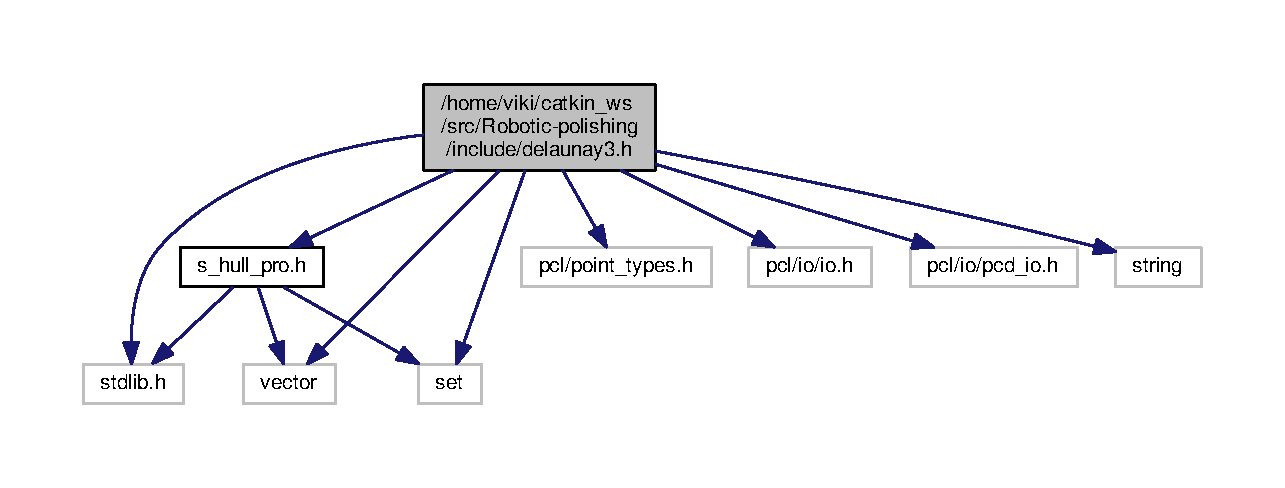
\includegraphics[width=350pt]{delaunay3_8h__incl}
\end{center}
\end{figure}
This graph shows which files directly or indirectly include this file\+:
\nopagebreak
\begin{figure}[H]
\begin{center}
\leavevmode
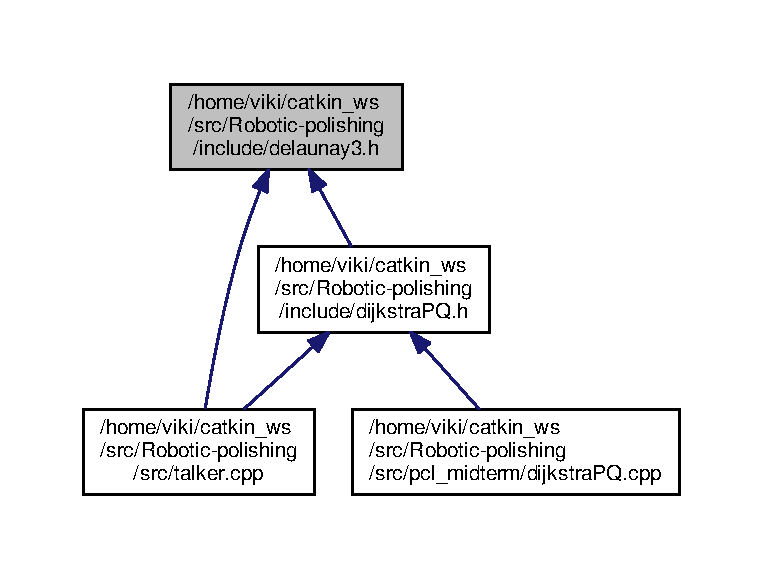
\includegraphics[width=350pt]{delaunay3_8h__dep__incl}
\end{center}
\end{figure}
\subsection*{Classes}
\begin{DoxyCompactItemize}
\item 
class \hyperlink{classdelaunay3}{delaunay3}
\begin{DoxyCompactList}\small\item\em This \hyperlink{delaunay3_8h}{delaunay3.\+h} is a header file of the meshing triangle among the point cloud. \end{DoxyCompactList}\end{DoxyCompactItemize}


\subsection{Detailed Description}
This \hyperlink{delaunay3_8h}{delaunay3.\+h} is a header file of the meshing triangle among the point cloud. 

This delaunay3.\+cpp is an implement file of the meshing triangle among the point cloud.

\begin{DoxyAuthor}{Author}
Michael Kam (michael081906) 
\end{DoxyAuthor}
\begin{DoxyRefDesc}{Bug}
\item[\hyperlink{bug__bug000001}{Bug}]No known bugs. \end{DoxyRefDesc}
\begin{DoxyCopyright}{Copyright}
G\+NU Public License.
\end{DoxyCopyright}
\hyperlink{classdelaunay3}{delaunay3} is free software\+: you can redistribute it and/or modify it under the terms of the G\+NU General Public License as published by the Free Software Foundation, either version 3 of the License, or (at your option) any later version.

\hyperlink{classdelaunay3}{delaunay3} is distributed in the hope that it will be useful, but W\+I\+T\+H\+O\+UT A\+NY W\+A\+R\+R\+A\+N\+TY; without even the implied warranty of M\+E\+R\+C\+H\+A\+N\+T\+A\+B\+I\+L\+I\+TY or F\+I\+T\+N\+E\+SS F\+OR A P\+A\+R\+T\+I\+C\+U\+L\+AR P\+U\+R\+P\+O\+SE. See the G\+NU General Public License for more details. You should have received a copy of the G\+NU General Public License along with \hyperlink{classdelaunay3}{delaunay3}. If not, see \href{http://www.gnu.org/licenses/}{\tt http\+://www.\+gnu.\+org/licenses/}.

\begin{DoxyAuthor}{Author}
Michael Kam (michael081906) 
\end{DoxyAuthor}
\begin{DoxyRefDesc}{Bug}
\item[\hyperlink{bug__bug000026}{Bug}]No known bugs. \end{DoxyRefDesc}
\begin{DoxyCopyright}{Copyright}
G\+NU Public License.
\end{DoxyCopyright}
\hyperlink{classdelaunay3}{delaunay3} is free software\+: you can redistribute it and/or modify it under the terms of the G\+NU General Public License as published by the Free Software Foundation, either version 3 of the License, or (at your option) any later version.

\hyperlink{classdelaunay3}{delaunay3} is distributed in the hope that it will be useful, but W\+I\+T\+H\+O\+UT A\+NY W\+A\+R\+R\+A\+N\+TY; without even the implied warranty of M\+E\+R\+C\+H\+A\+N\+T\+A\+B\+I\+L\+I\+TY or F\+I\+T\+N\+E\+SS F\+OR A P\+A\+R\+T\+I\+C\+U\+L\+AR P\+U\+R\+P\+O\+SE. See the G\+NU General Public License for more details. You should have received a copy of the G\+NU General Public License along with \hyperlink{classdelaunay3}{delaunay3}. If not, see \href{http://www.gnu.org/licenses/}{\tt http\+://www.\+gnu.\+org/licenses/}. 
\hypertarget{dijkstraPQ_8h}{}\section{/home/viki/catkin\+\_\+ws/src/\+Robotic-\/polishing/include/dijkstra\+PQ.h File Reference}
\label{dijkstraPQ_8h}\index{/home/viki/catkin\+\_\+ws/src/\+Robotic-\/polishing/include/dijkstra\+P\+Q.\+h@{/home/viki/catkin\+\_\+ws/src/\+Robotic-\/polishing/include/dijkstra\+P\+Q.\+h}}


This \hyperlink{dijkstraPQ_8cpp}{dijkstra\+P\+Q.\+cpp} is a header file of finding shortest path among the point cloud. The algorithm refer to here\+: \href{http://www.geeksforgeeks.org/dijkstras-shortest-path-algorithm-using-priority_queue-stl/}{\tt http\+://www.\+geeksforgeeks.\+org/dijkstras-\/shortest-\/path-\/algorithm-\/using-\/priority\+\_\+queue-\/stl/}.  


{\ttfamily \#include $<$vector$>$}\\*
{\ttfamily \#include $<$pcl/point\+\_\+types.\+h$>$}\\*
{\ttfamily \#include $<$pcl/io/io.\+h$>$}\\*
{\ttfamily \#include $<$delaunay3.\+h$>$}\\*
Include dependency graph for dijkstra\+P\+Q.\+h\+:
\nopagebreak
\begin{figure}[H]
\begin{center}
\leavevmode
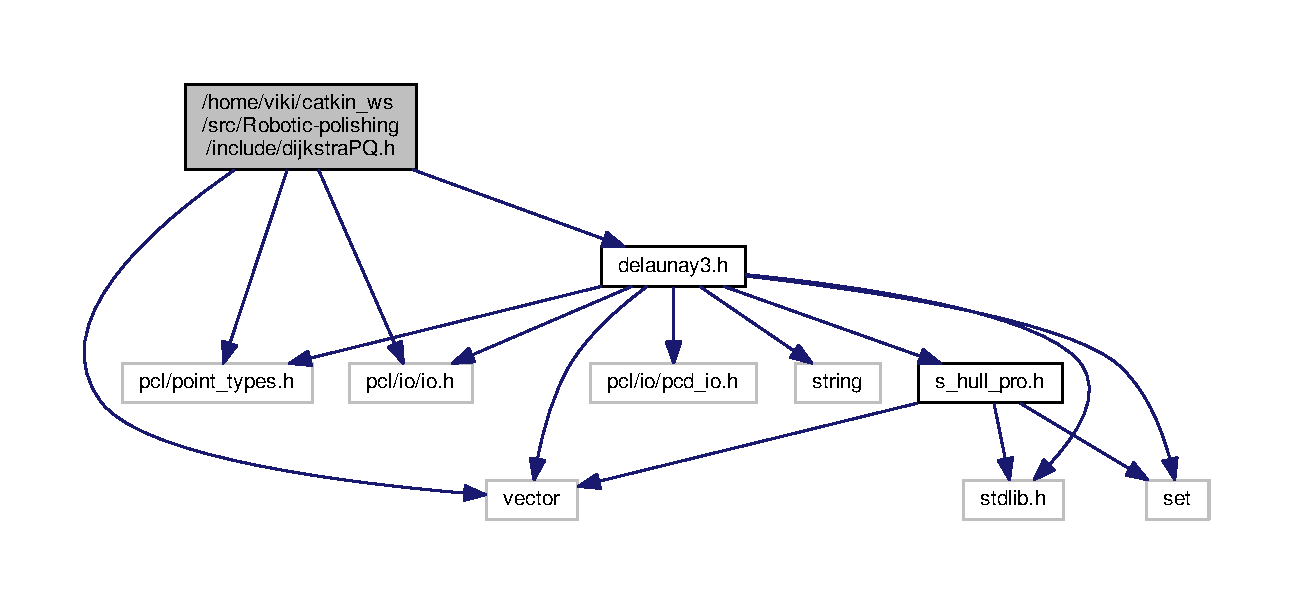
\includegraphics[width=350pt]{dijkstraPQ_8h__incl}
\end{center}
\end{figure}
This graph shows which files directly or indirectly include this file\+:
\nopagebreak
\begin{figure}[H]
\begin{center}
\leavevmode
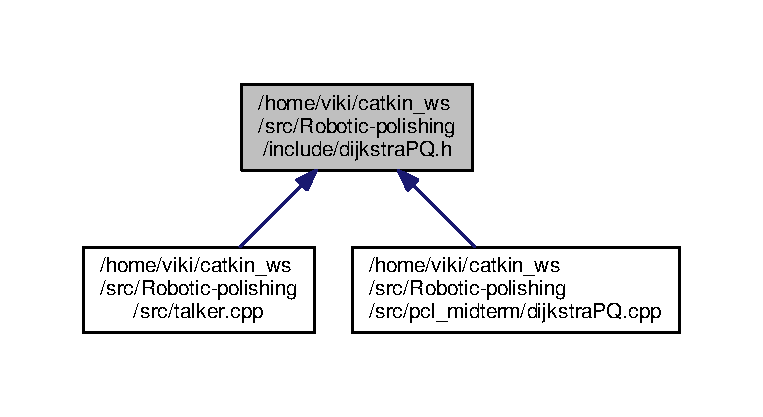
\includegraphics[width=350pt]{dijkstraPQ_8h__dep__incl}
\end{center}
\end{figure}
\subsection*{Classes}
\begin{DoxyCompactItemize}
\item 
struct \hyperlink{structposition}{position}
\item 
class \hyperlink{classdijkstraPQ}{dijkstra\+PQ}
\begin{DoxyCompactList}\small\item\em \hyperlink{classkukaControl}{kuka\+Control} is a header file of finding shortest path among the point cloud. \end{DoxyCompactList}\end{DoxyCompactItemize}
\subsection*{Typedefs}
\begin{DoxyCompactItemize}
\item 
typedef std\+::pair$<$ int, double $>$ {\bfseries i\+Pair}\hypertarget{dijkstraPQ_8h_a624600417e5ffc98a4bd14a6d109d21c}{}\label{dijkstraPQ_8h_a624600417e5ffc98a4bd14a6d109d21c}

\end{DoxyCompactItemize}


\subsection{Detailed Description}
This \hyperlink{dijkstraPQ_8cpp}{dijkstra\+P\+Q.\+cpp} is a header file of finding shortest path among the point cloud. The algorithm refer to here\+: \href{http://www.geeksforgeeks.org/dijkstras-shortest-path-algorithm-using-priority_queue-stl/}{\tt http\+://www.\+geeksforgeeks.\+org/dijkstras-\/shortest-\/path-\/algorithm-\/using-\/priority\+\_\+queue-\/stl/}. 

\begin{DoxyAuthor}{Author}
Michael Kam (michael081906) 
\end{DoxyAuthor}
\begin{DoxyRefDesc}{Bug}
\item[\hyperlink{bug__bug000003}{Bug}]No known bugs. \end{DoxyRefDesc}
\begin{DoxyCopyright}{Copyright}
G\+NU Public License.
\end{DoxyCopyright}
\hyperlink{classdijkstraPQ}{dijkstra\+PQ} is free software\+: you can redistribute it and/or modify it under the terms of the G\+NU General Public License as published by the Free Software Foundation, either version 3 of the License, or (at your option) any later version.

\hyperlink{classdijkstraPQ}{dijkstra\+PQ} is distributed in the hope that it will be useful, but W\+I\+T\+H\+O\+UT A\+NY W\+A\+R\+R\+A\+N\+TY; without even the implied warranty of M\+E\+R\+C\+H\+A\+N\+T\+A\+B\+I\+L\+I\+TY or F\+I\+T\+N\+E\+SS F\+OR A P\+A\+R\+T\+I\+C\+U\+L\+AR P\+U\+R\+P\+O\+SE. See the G\+NU General Public License for more details. You should have received a copy of the G\+NU General Public License along with \hyperlink{classdijkstraPQ}{dijkstra\+PQ}. If not, see \href{http://www.gnu.org/licenses/}{\tt http\+://www.\+gnu.\+org/licenses/}. 
\hypertarget{kukaControl_8h}{}\section{/home/viki/catkin\+\_\+ws/src/\+Robotic-\/polishing/include/kuka\+Control.h File Reference}
\label{kukaControl_8h}\index{/home/viki/catkin\+\_\+ws/src/\+Robotic-\/polishing/include/kuka\+Control.\+h@{/home/viki/catkin\+\_\+ws/src/\+Robotic-\/polishing/include/kuka\+Control.\+h}}


This \hyperlink{kukaControl_8h}{kuka\+Control.\+h} is a header file of controlling the iiwa kuka arm.  


{\ttfamily \#include $<$ros/ros.\+h$>$}\\*
{\ttfamily \#include $<$trajectory\+\_\+msgs/\+Joint\+Trajectory.\+h$>$}\\*
{\ttfamily \#include $<$trajectory\+\_\+msgs/\+Joint\+Trajectory\+Point.\+h$>$}\\*
{\ttfamily \#include $<$geometry\+\_\+msgs/\+Twist.\+h$>$}\\*
{\ttfamily \#include $<$iiwa\+\_\+msgs/\+Joint\+Position.\+h$>$}\\*
{\ttfamily \#include $<$sensor\+\_\+msgs/\+Joint\+State.\+h$>$}\\*
{\ttfamily \#include $<$kdl/chain.\+hpp$>$}\\*
{\ttfamily \#include \char`\"{}Eigen/\+Core\char`\"{}}\\*
{\ttfamily \#include $<$kdl/chainfksolver.\+hpp$>$}\\*
{\ttfamily \#include $<$kdl/chainiksolver.\+hpp$>$}\\*
{\ttfamily \#include $<$kdl/chainfksolverpos\+\_\+recursive.\+hpp$>$}\\*
{\ttfamily \#include $<$kdl/chainiksolvervel\+\_\+pinv.\+hpp$>$}\\*
{\ttfamily \#include $<$kdl/chainiksolverpos\+\_\+nr.\+hpp$>$}\\*
{\ttfamily \#include $<$kdl/chainjnttojacsolver.\+hpp$>$}\\*
{\ttfamily \#include $<$string$>$}\\*
{\ttfamily \#include $<$sstream$>$}\\*
Include dependency graph for kuka\+Control.\+h\+:
\nopagebreak
\begin{figure}[H]
\begin{center}
\leavevmode
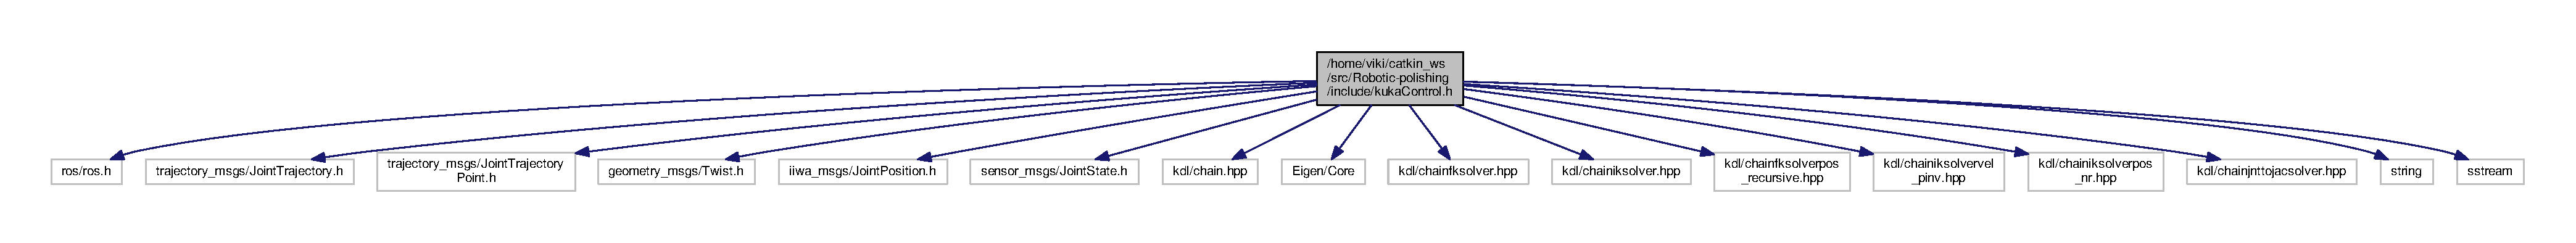
\includegraphics[width=350pt]{kukaControl_8h__incl}
\end{center}
\end{figure}
This graph shows which files directly or indirectly include this file\+:
\nopagebreak
\begin{figure}[H]
\begin{center}
\leavevmode
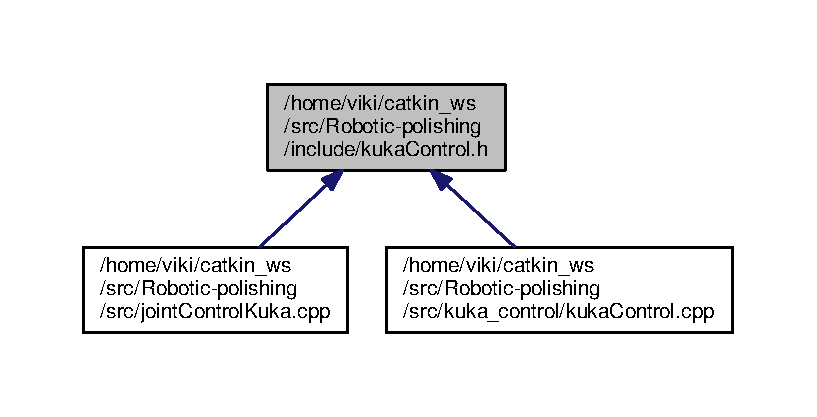
\includegraphics[width=350pt]{kukaControl_8h__dep__incl}
\end{center}
\end{figure}
\subsection*{Classes}
\begin{DoxyCompactItemize}
\item 
class \hyperlink{classkukaControl}{kuka\+Control}
\begin{DoxyCompactList}\small\item\em \hyperlink{classkukaControl}{kuka\+Control} is an implementation of controlling the iiwa kuka arm
\begin{DoxyItemize}
\item 
\end{DoxyItemize}\end{DoxyCompactList}\end{DoxyCompactItemize}


\subsection{Detailed Description}
This \hyperlink{kukaControl_8h}{kuka\+Control.\+h} is a header file of controlling the iiwa kuka arm. 

\begin{DoxyAuthor}{Author}
Michael Kam (michael081906) 
\end{DoxyAuthor}
\begin{DoxyRefDesc}{Bug}
\item[\hyperlink{bug__bug000007}{Bug}]No known bugs. \end{DoxyRefDesc}
\begin{DoxyCopyright}{Copyright}
G\+NU Public License.
\end{DoxyCopyright}
\hyperlink{classkukaControl}{kuka\+Control} is free software\+: you can redistribute it and/or modify it under the terms of the G\+NU General Public License as published by the Free Software Foundation, either version 3 of the License, or (at your option) any later version.

\hyperlink{classkukaControl}{kuka\+Control} is distributed in the hope that it will be useful, but W\+I\+T\+H\+O\+UT A\+NY W\+A\+R\+R\+A\+N\+TY; without even the implied warranty of M\+E\+R\+C\+H\+A\+N\+T\+A\+B\+I\+L\+I\+TY or F\+I\+T\+N\+E\+SS F\+OR A P\+A\+R\+T\+I\+C\+U\+L\+AR P\+U\+R\+P\+O\+SE. See the G\+NU General Public License for more details. You should have received a copy of the G\+NU General Public License along with \hyperlink{classkukaControl}{kuka\+Control}. If not, see \href{http://www.gnu.org/licenses/}{\tt http\+://www.\+gnu.\+org/licenses/}. 
\hypertarget{pclCloudViewer_8h}{}\section{/home/viki/catkin\+\_\+ws/src/\+Robotic-\/polishing/include/pcl\+Cloud\+Viewer.h File Reference}
\label{pclCloudViewer_8h}\index{/home/viki/catkin\+\_\+ws/src/\+Robotic-\/polishing/include/pcl\+Cloud\+Viewer.\+h@{/home/viki/catkin\+\_\+ws/src/\+Robotic-\/polishing/include/pcl\+Cloud\+Viewer.\+h}}


header file of an \hyperlink{classpclCloudViewer}{pcl\+Cloud\+Viewer} class.  


{\ttfamily \#include $<$pcl/visualization/cloud\+\_\+viewer.\+h$>$}\\*
{\ttfamily \#include $<$pcl/io/io.\+h$>$}\\*
{\ttfamily \#include $<$pcl/io/pcd\+\_\+io.\+h$>$}\\*
{\ttfamily \#include $<$pcl/point\+\_\+types.\+h$>$}\\*
{\ttfamily \#include $<$iostream$>$}\\*
Include dependency graph for pcl\+Cloud\+Viewer.\+h\+:
\nopagebreak
\begin{figure}[H]
\begin{center}
\leavevmode
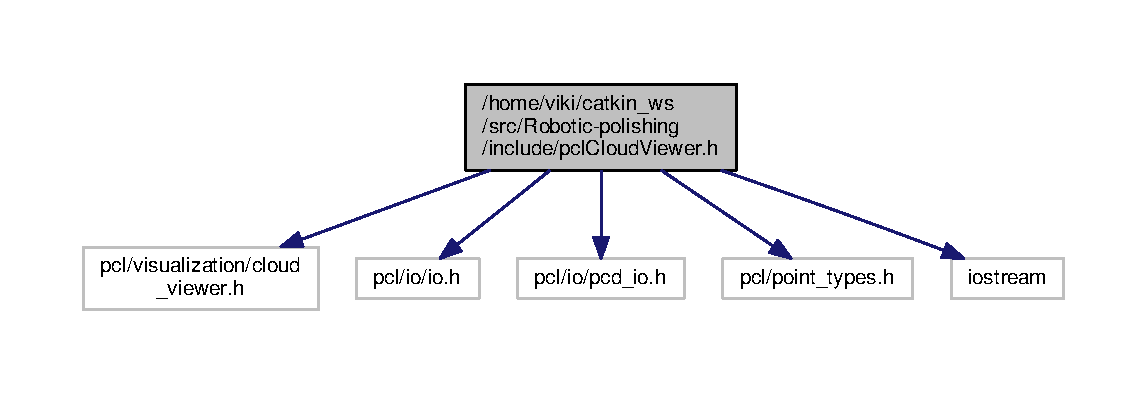
\includegraphics[width=350pt]{pclCloudViewer_8h__incl}
\end{center}
\end{figure}
This graph shows which files directly or indirectly include this file\+:
\nopagebreak
\begin{figure}[H]
\begin{center}
\leavevmode
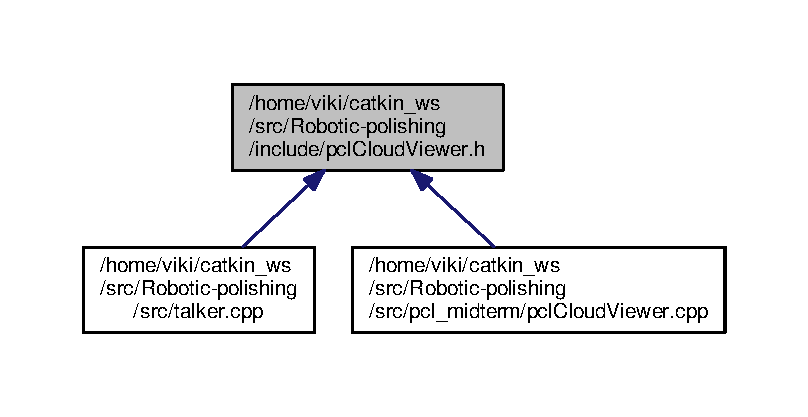
\includegraphics[width=350pt]{pclCloudViewer_8h__dep__incl}
\end{center}
\end{figure}
\subsection*{Classes}
\begin{DoxyCompactItemize}
\item 
class \hyperlink{classpclCloudViewer}{pcl\+Cloud\+Viewer}
\begin{DoxyCompactList}\small\item\em \hyperlink{classpclCloudViewer}{pcl\+Cloud\+Viewer} is an implementation by using pcl visualization to display the point cloud
\begin{DoxyItemize}
\item 
\end{DoxyItemize}\end{DoxyCompactList}\end{DoxyCompactItemize}


\subsection{Detailed Description}
header file of an \hyperlink{classpclCloudViewer}{pcl\+Cloud\+Viewer} class. 

This class utilize pcl visualization to display point cloud.

\begin{DoxyAuthor}{Author}
Michael Kam (michael081906) 
\end{DoxyAuthor}
\begin{DoxyRefDesc}{Bug}
\item[\hyperlink{bug__bug000009}{Bug}]No1 can\textquotesingle{}t not be compile successfully in the test case. \end{DoxyRefDesc}
\begin{DoxyCopyright}{Copyright}
G\+NU Public License.
\end{DoxyCopyright}
\hyperlink{classpclCloudViewer}{pcl\+Cloud\+Viewer} is free software\+: you can redistribute it and/or modify it under the terms of the G\+NU General Public License as published by the Free Software Foundation, either version 3 of the License, or (at your option) any later version.

\hyperlink{classpclCloudViewer}{pcl\+Cloud\+Viewer} is distributed in the hope that it will be useful, but W\+I\+T\+H\+O\+UT A\+NY W\+A\+R\+R\+A\+N\+TY; without even the implied warranty of M\+E\+R\+C\+H\+A\+N\+T\+A\+B\+I\+L\+I\+TY or F\+I\+T\+N\+E\+SS F\+OR A P\+A\+R\+T\+I\+C\+U\+L\+AR P\+U\+R\+P\+O\+SE. See the G\+NU General Public License for more details. You should have received a copy of the G\+NU General Public License along with \hyperlink{classpclCloudViewer}{pcl\+Cloud\+Viewer}. If not, see \href{http://www.gnu.org/licenses/}{\tt http\+://www.\+gnu.\+org/licenses/}. $\ast$ 
\hypertarget{pclFastTriangular_8h}{}\section{/home/viki/catkin\+\_\+ws/src/\+Robotic-\/polishing/include/pcl\+Fast\+Triangular.h File Reference}
\label{pclFastTriangular_8h}\index{/home/viki/catkin\+\_\+ws/src/\+Robotic-\/polishing/include/pcl\+Fast\+Triangular.\+h@{/home/viki/catkin\+\_\+ws/src/\+Robotic-\/polishing/include/pcl\+Fast\+Triangular.\+h}}


header file of an \hyperlink{classpclFastTriangular}{pcl\+Fast\+Triangular} class.  


{\ttfamily \#include $<$pcl/io/io.\+h$>$}\\*
{\ttfamily \#include $<$pcl/io/pcd\+\_\+io.\+h$>$}\\*
{\ttfamily \#include $<$pcl/point\+\_\+types.\+h$>$}\\*
{\ttfamily \#include $<$pcl/kdtree/kdtree\+\_\+flann.\+h$>$}\\*
{\ttfamily \#include $<$pcl/features/normal\+\_\+3d.\+h$>$}\\*
{\ttfamily \#include $<$pcl/surface/gp3.\+h$>$}\\*
{\ttfamily \#include $<$iostream$>$}\\*
{\ttfamily \#include $<$vector$>$}\\*
{\ttfamily \#include $<$ios$>$}\\*
Include dependency graph for pcl\+Fast\+Triangular.\+h\+:
\nopagebreak
\begin{figure}[H]
\begin{center}
\leavevmode
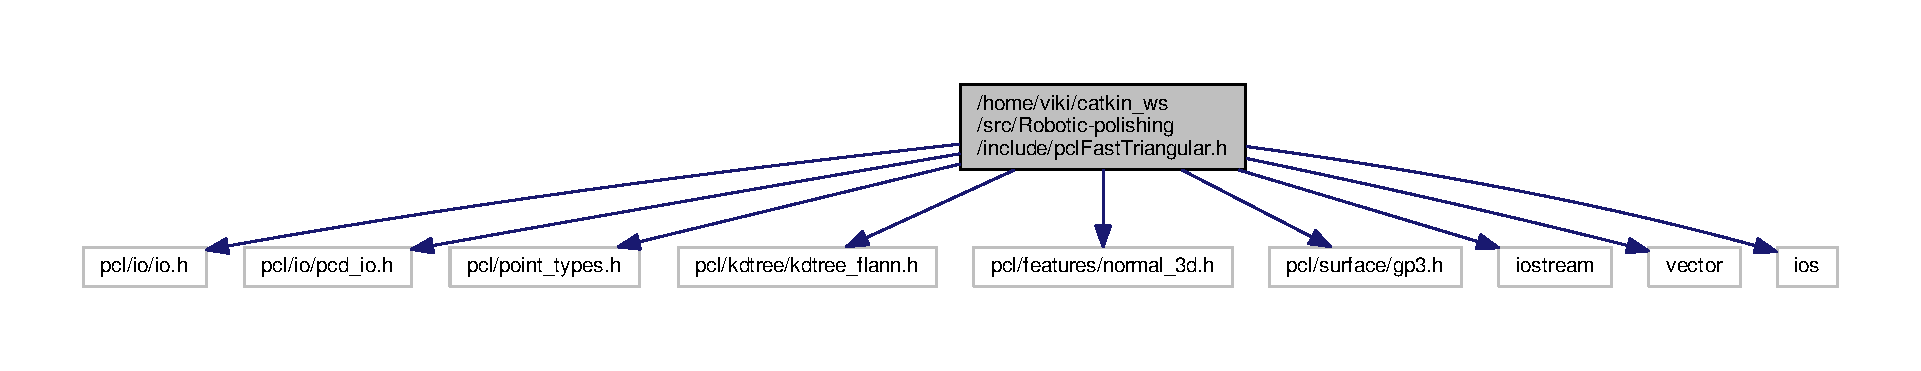
\includegraphics[width=350pt]{pclFastTriangular_8h__incl}
\end{center}
\end{figure}
This graph shows which files directly or indirectly include this file\+:
\nopagebreak
\begin{figure}[H]
\begin{center}
\leavevmode
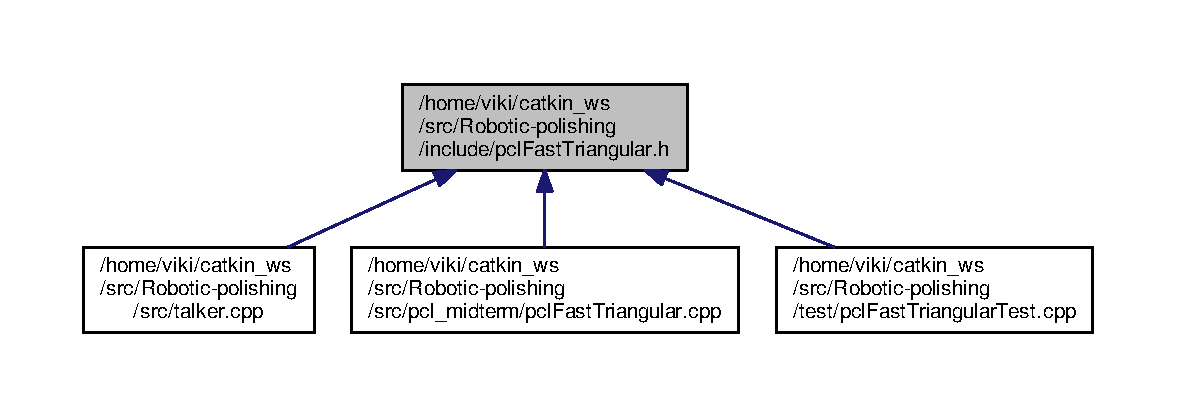
\includegraphics[width=350pt]{pclFastTriangular_8h__dep__incl}
\end{center}
\end{figure}
\subsection*{Classes}
\begin{DoxyCompactItemize}
\item 
class \hyperlink{classpclFastTriangular}{pcl\+Fast\+Triangular}
\begin{DoxyCompactList}\small\item\em \hyperlink{classpclFastTriangular}{pcl\+Fast\+Triangular} is an implementation by using pcl fast\+Triangular method to reconstruct the surface.
\begin{DoxyItemize}
\item 
\end{DoxyItemize}\end{DoxyCompactList}\end{DoxyCompactItemize}


\subsection{Detailed Description}
header file of an \hyperlink{classpclFastTriangular}{pcl\+Fast\+Triangular} class. 

This class utilizes pcl fast\+Triangular method to reconstruct the surface.

\begin{DoxyAuthor}{Author}
Michael Kam (michael081906) 
\end{DoxyAuthor}
\begin{DoxyRefDesc}{Bug}
\item[\hyperlink{bug__bug000011}{Bug}]No known bugs. \end{DoxyRefDesc}
\begin{DoxyCopyright}{Copyright}
G\+NU Public License.
\end{DoxyCopyright}
\hyperlink{classpclFastTriangular}{pcl\+Fast\+Triangular} is free software\+: you can redistribute it and/or modify it under the terms of the G\+NU General Public License as published by the Free Software Foundation, either version 3 of the License, or (at your option) any later version.

\hyperlink{classpclFastTriangular}{pcl\+Fast\+Triangular} is distributed in the hope that it will be useful, but W\+I\+T\+H\+O\+UT A\+NY W\+A\+R\+R\+A\+N\+TY; without even the implied warranty of M\+E\+R\+C\+H\+A\+N\+T\+A\+B\+I\+L\+I\+TY or F\+I\+T\+N\+E\+SS F\+OR A P\+A\+R\+T\+I\+C\+U\+L\+AR P\+U\+R\+P\+O\+SE. See the G\+NU General Public License for more details. You should have received a copy of the G\+NU General Public License along with \hyperlink{classpclFastTriangular}{pcl\+Fast\+Triangular}. If not, see \href{http://www.gnu.org/licenses/}{\tt http\+://www.\+gnu.\+org/licenses/}. 
\hypertarget{pclIo_8h}{}\section{/home/viki/catkin\+\_\+ws/src/\+Robotic-\/polishing/include/pcl\+Io.h File Reference}
\label{pclIo_8h}\index{/home/viki/catkin\+\_\+ws/src/\+Robotic-\/polishing/include/pcl\+Io.\+h@{/home/viki/catkin\+\_\+ws/src/\+Robotic-\/polishing/include/pcl\+Io.\+h}}


header file of an \hyperlink{classpclIo}{pcl\+Io} class.  


{\ttfamily \#include $<$pcl/io/io.\+h$>$}\\*
{\ttfamily \#include $<$pcl/io/pcd\+\_\+io.\+h$>$}\\*
{\ttfamily \#include $<$pcl/point\+\_\+types.\+h$>$}\\*
{\ttfamily \#include $<$iostream$>$}\\*
{\ttfamily \#include $<$string$>$}\\*
Include dependency graph for pcl\+Io.\+h\+:
\nopagebreak
\begin{figure}[H]
\begin{center}
\leavevmode
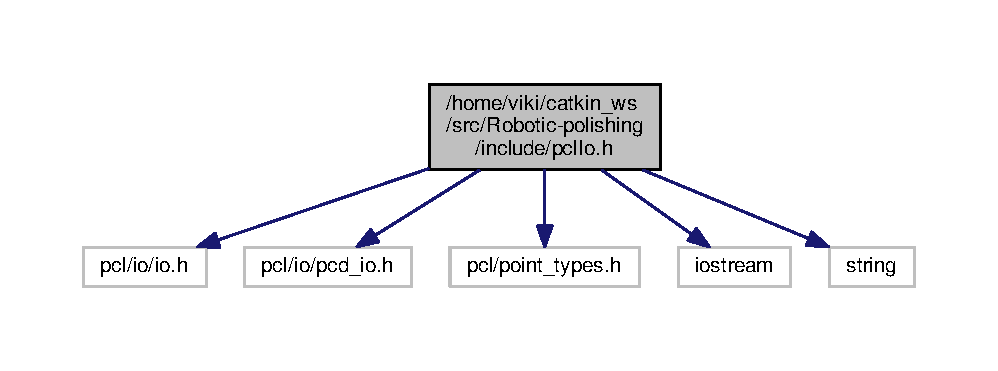
\includegraphics[width=350pt]{pclIo_8h__incl}
\end{center}
\end{figure}
This graph shows which files directly or indirectly include this file\+:
\nopagebreak
\begin{figure}[H]
\begin{center}
\leavevmode
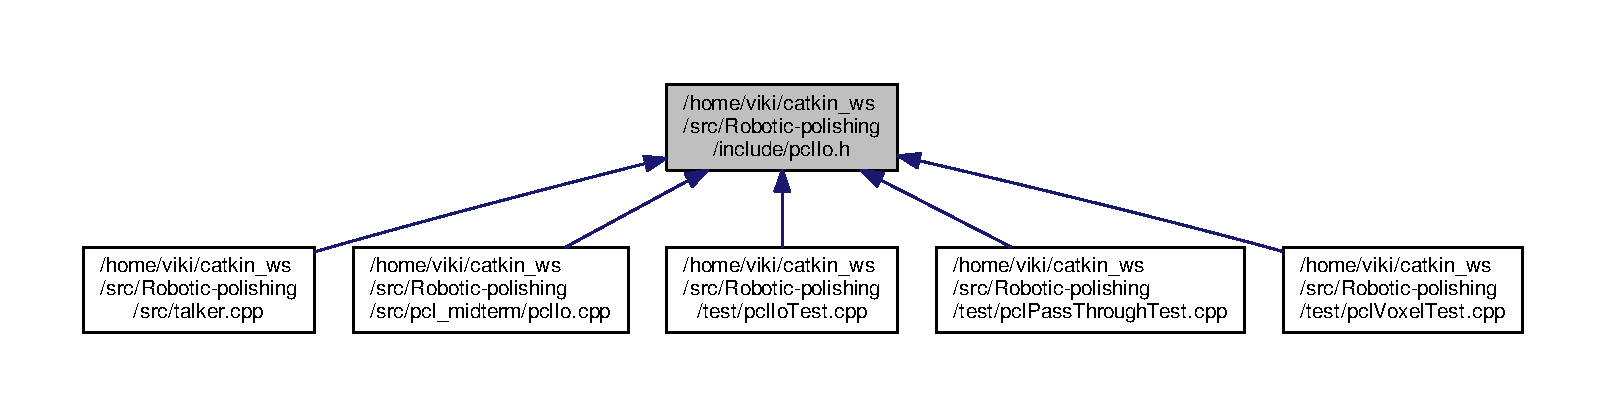
\includegraphics[width=350pt]{pclIo_8h__dep__incl}
\end{center}
\end{figure}
\subsection*{Classes}
\begin{DoxyCompactItemize}
\item 
class \hyperlink{classpclIo}{pcl\+Io}
\begin{DoxyCompactList}\small\item\em \hyperlink{classpclIo}{pcl\+Io} is an implementation by using pcl to load .pcd file from local.
\begin{DoxyItemize}
\item 
\end{DoxyItemize}\end{DoxyCompactList}\end{DoxyCompactItemize}


\subsection{Detailed Description}
header file of an \hyperlink{classpclIo}{pcl\+Io} class. 

This class utilizes pcl to load .pcd file from local.

\begin{DoxyAuthor}{Author}
Michael Kam (michael081906) 
\end{DoxyAuthor}
\begin{DoxyRefDesc}{Bug}
\item[\hyperlink{bug__bug000013}{Bug}]No known bugs. \end{DoxyRefDesc}
\begin{DoxyCopyright}{Copyright}
G\+NU Public License.
\end{DoxyCopyright}
\hyperlink{classpclIo}{pcl\+Io} is free software\+: you can redistribute it and/or modify it under the terms of the G\+NU General Public License as published by the Free Software Foundation, either version 3 of the License, or (at your option) any later version.

\hyperlink{classpclIo}{pcl\+Io} is distributed in the hope that it will be useful, but W\+I\+T\+H\+O\+UT A\+NY W\+A\+R\+R\+A\+N\+TY; without even the implied warranty of M\+E\+R\+C\+H\+A\+N\+T\+A\+B\+I\+L\+I\+TY or F\+I\+T\+N\+E\+SS F\+OR A P\+A\+R\+T\+I\+C\+U\+L\+AR P\+U\+R\+P\+O\+SE. See the G\+NU General Public License for more details. You should have received a copy of the G\+NU General Public License along with \hyperlink{classpclIo}{pcl\+Io}. If not, see \href{http://www.gnu.org/licenses/}{\tt http\+://www.\+gnu.\+org/licenses/}. 
\hypertarget{pclMlsSmoothing_8h}{}\section{/home/viki/catkin\+\_\+ws/src/\+Robotic-\/polishing/include/pcl\+Mls\+Smoothing.h File Reference}
\label{pclMlsSmoothing_8h}\index{/home/viki/catkin\+\_\+ws/src/\+Robotic-\/polishing/include/pcl\+Mls\+Smoothing.\+h@{/home/viki/catkin\+\_\+ws/src/\+Robotic-\/polishing/include/pcl\+Mls\+Smoothing.\+h}}


header file of an \hyperlink{classpclMlsSmoothing}{pcl\+Mls\+Smoothing} class  


{\ttfamily \#include $<$pcl/io/io.\+h$>$}\\*
{\ttfamily \#include $<$pcl/io/pcd\+\_\+io.\+h$>$}\\*
{\ttfamily \#include $<$pcl/point\+\_\+types.\+h$>$}\\*
{\ttfamily \#include $<$pcl/kdtree/kdtree\+\_\+flann.\+h$>$}\\*
{\ttfamily \#include $<$pcl/surface/mls.\+h$>$}\\*
{\ttfamily \#include $<$iostream$>$}\\*
{\ttfamily \#include $<$vector$>$}\\*
{\ttfamily \#include $<$ios$>$}\\*
Include dependency graph for pcl\+Mls\+Smoothing.\+h\+:
\nopagebreak
\begin{figure}[H]
\begin{center}
\leavevmode
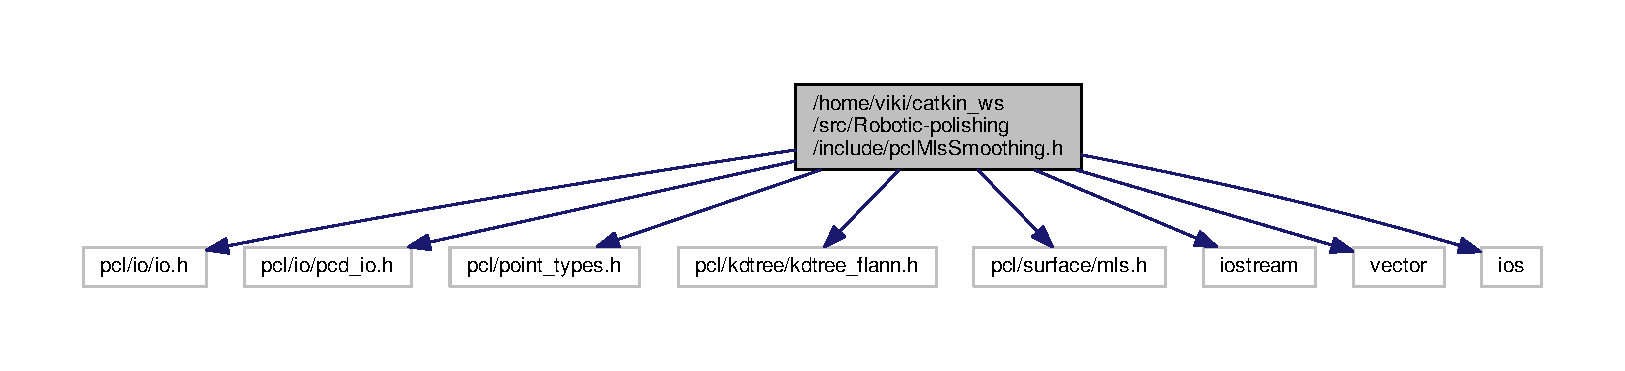
\includegraphics[width=350pt]{pclMlsSmoothing_8h__incl}
\end{center}
\end{figure}
This graph shows which files directly or indirectly include this file\+:
\nopagebreak
\begin{figure}[H]
\begin{center}
\leavevmode
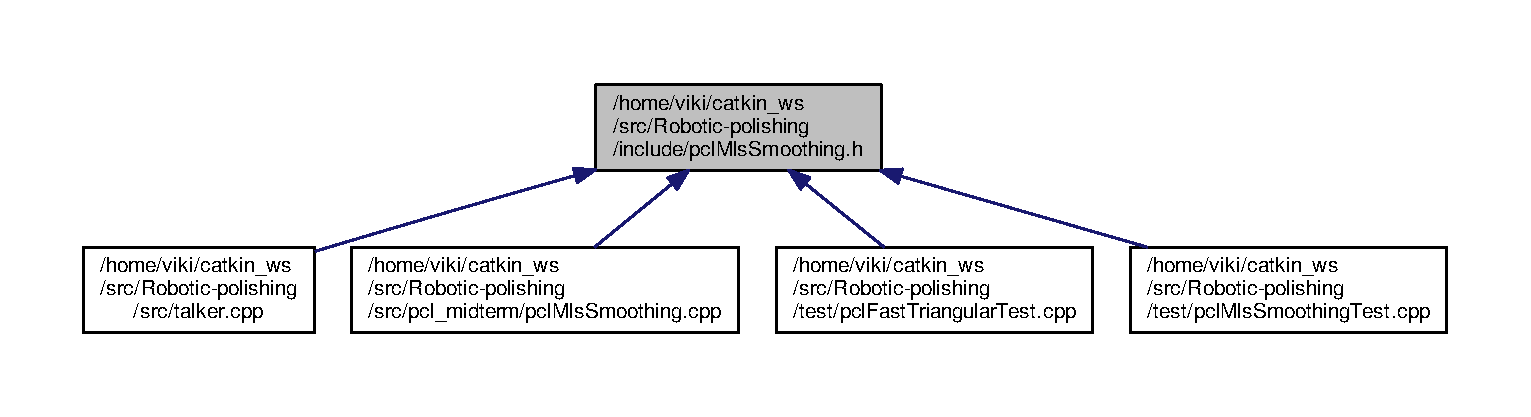
\includegraphics[width=350pt]{pclMlsSmoothing_8h__dep__incl}
\end{center}
\end{figure}
\subsection*{Classes}
\begin{DoxyCompactItemize}
\item 
class \hyperlink{classpclMlsSmoothing}{pcl\+Mls\+Smoothing}
\begin{DoxyCompactList}\small\item\em \hyperlink{classpclMlsSmoothing}{pcl\+Mls\+Smoothing} is an implementation by using moving least square(mls) method to smooth the point cloud among the surface. \end{DoxyCompactList}\end{DoxyCompactItemize}


\subsection{Detailed Description}
header file of an \hyperlink{classpclMlsSmoothing}{pcl\+Mls\+Smoothing} class 

This class utilizes pcl moving least square(mls) method to smooth the point cloud among the surface.

\begin{DoxyAuthor}{Author}
Michael Kam (michael081906) 
\end{DoxyAuthor}
\begin{DoxyRefDesc}{Bug}
\item[\hyperlink{bug__bug000015}{Bug}]No known bugs. \end{DoxyRefDesc}
\begin{DoxyCopyright}{Copyright}
G\+NU Public License.
\end{DoxyCopyright}
\hyperlink{classpclMlsSmoothing}{pcl\+Mls\+Smoothing} is free software\+: you can redistribute it and/or modify it under the terms of the G\+NU General Public License as published by the Free Software Foundation, either version 3 of the License, or (at your option) any later version.

\hyperlink{classpclMlsSmoothing}{pcl\+Mls\+Smoothing} is distributed in the hope that it will be useful, but W\+I\+T\+H\+O\+UT A\+NY W\+A\+R\+R\+A\+N\+TY; without even the implied warranty of M\+E\+R\+C\+H\+A\+N\+T\+A\+B\+I\+L\+I\+TY or F\+I\+T\+N\+E\+SS F\+OR A P\+A\+R\+T\+I\+C\+U\+L\+AR P\+U\+R\+P\+O\+SE. See the G\+NU General Public License for more details. You should have received a copy of the G\+NU General Public License along with \hyperlink{classpclMlsSmoothing}{pcl\+Mls\+Smoothing}. If not, see \href{http://www.gnu.org/licenses/}{\tt http\+://www.\+gnu.\+org/licenses/}. 
\hypertarget{pclVoxel_8h}{}\section{/home/viki/catkin\+\_\+ws/src/\+Robotic-\/polishing/include/pcl\+Voxel.h File Reference}
\label{pclVoxel_8h}\index{/home/viki/catkin\+\_\+ws/src/\+Robotic-\/polishing/include/pcl\+Voxel.\+h@{/home/viki/catkin\+\_\+ws/src/\+Robotic-\/polishing/include/pcl\+Voxel.\+h}}


header file of an \hyperlink{classpclVoxel}{pcl\+Voxel} class.  


{\ttfamily \#include $<$pcl/io/io.\+h$>$}\\*
{\ttfamily \#include $<$pcl/io/pcd\+\_\+io.\+h$>$}\\*
{\ttfamily \#include $<$pcl/point\+\_\+types.\+h$>$}\\*
{\ttfamily \#include $<$pcl/filters/voxel\+\_\+grid.\+h$>$}\\*
{\ttfamily \#include $<$vector$>$}\\*
{\ttfamily \#include $<$iostream$>$}\\*
{\ttfamily \#include $<$ios$>$}\\*
Include dependency graph for pcl\+Voxel.\+h\+:
\nopagebreak
\begin{figure}[H]
\begin{center}
\leavevmode
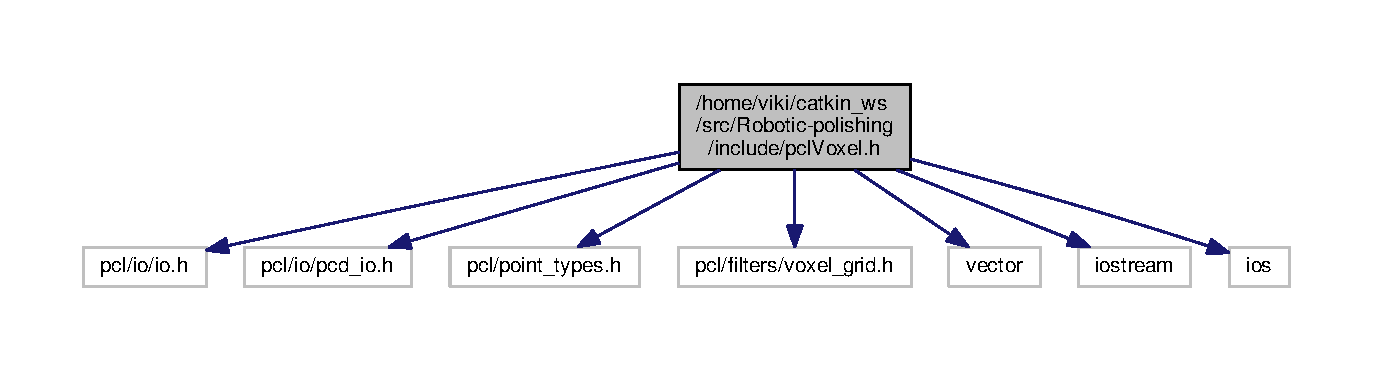
\includegraphics[width=350pt]{pclVoxel_8h__incl}
\end{center}
\end{figure}
This graph shows which files directly or indirectly include this file\+:
\nopagebreak
\begin{figure}[H]
\begin{center}
\leavevmode
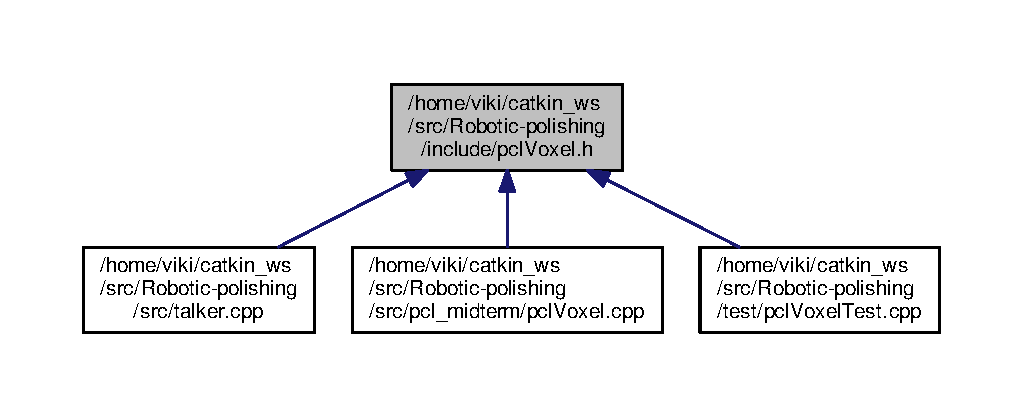
\includegraphics[width=350pt]{pclVoxel_8h__dep__incl}
\end{center}
\end{figure}
\subsection*{Classes}
\begin{DoxyCompactItemize}
\item 
class \hyperlink{classpclVoxel}{pcl\+Voxel}
\begin{DoxyCompactList}\small\item\em \hyperlink{classpclVoxel}{pcl\+Voxel} is an implementation by using pcl voxel\+\_\+grid filter to down sample the point cloud
\begin{DoxyItemize}
\item 
\end{DoxyItemize}\end{DoxyCompactList}\end{DoxyCompactItemize}


\subsection{Detailed Description}
header file of an \hyperlink{classpclVoxel}{pcl\+Voxel} class. 

This class utilize pcl voxel\+\_\+grid filter to down sample the point cloud.

\begin{DoxyAuthor}{Author}
Michael Kam (michael081906) 
\end{DoxyAuthor}
\begin{DoxyRefDesc}{Bug}
\item[\hyperlink{bug__bug000021}{Bug}]No known bugs. \end{DoxyRefDesc}
\begin{DoxyCopyright}{Copyright}
G\+NU Public License.
\end{DoxyCopyright}
\hyperlink{classpclVoxel}{pcl\+Voxel} is free software\+: you can redistribute it and/or modify it under the terms of the G\+NU General Public License as published by the Free Software Foundation, either version 3 of the License, or (at your option) any later version.

\hyperlink{classpclVoxel}{pcl\+Voxel} is distributed in the hope that it will be useful, but W\+I\+T\+H\+O\+UT A\+NY W\+A\+R\+R\+A\+N\+TY; without even the implied warranty of M\+E\+R\+C\+H\+A\+N\+T\+A\+B\+I\+L\+I\+TY or F\+I\+T\+N\+E\+SS F\+OR A P\+A\+R\+T\+I\+C\+U\+L\+AR P\+U\+R\+P\+O\+SE. See the G\+NU General Public License for more details. You should have received a copy of the G\+NU General Public License along with \hyperlink{classpclVoxel}{pcl\+Voxel}. If not, see \href{http://www.gnu.org/licenses/}{\tt http\+://www.\+gnu.\+org/licenses/}. 
\hypertarget{jointControlKuka_8cpp}{}\section{/home/viki/catkin\+\_\+ws/src/\+Robotic-\/polishing/src/joint\+Control\+Kuka.cpp File Reference}
\label{jointControlKuka_8cpp}\index{/home/viki/catkin\+\_\+ws/src/\+Robotic-\/polishing/src/joint\+Control\+Kuka.\+cpp@{/home/viki/catkin\+\_\+ws/src/\+Robotic-\/polishing/src/joint\+Control\+Kuka.\+cpp}}


This \hyperlink{jointControlKuka_8cpp}{joint\+Control\+Kuka.\+cpp} is a ros node that use to control the iiwa in gazebo.  


{\ttfamily \#include \char`\"{}kuka\+Control.\+h\char`\"{}}\\*
{\ttfamily \#include $<$ros/ros.\+h$>$}\\*
{\ttfamily \#include $<$trajectory\+\_\+msgs/\+Joint\+Trajectory.\+h$>$}\\*
{\ttfamily \#include $<$trajectory\+\_\+msgs/\+Joint\+Trajectory\+Point.\+h$>$}\\*
{\ttfamily \#include \char`\"{}robotic\+\_\+polishing/\+Trajectory.\+h\char`\"{}}\\*
{\ttfamily \#include $<$geometry\+\_\+msgs/\+Twist.\+h$>$}\\*
{\ttfamily \#include $<$iiwa\+\_\+msgs/\+Joint\+Position.\+h$>$}\\*
{\ttfamily \#include $<$sensor\+\_\+msgs/\+Joint\+State.\+h$>$}\\*
{\ttfamily \#include $<$kdl/chain.\+hpp$>$}\\*
{\ttfamily \#include \char`\"{}Eigen/\+Core\char`\"{}}\\*
{\ttfamily \#include $<$kdl/chainfksolver.\+hpp$>$}\\*
{\ttfamily \#include $<$kdl/chainiksolver.\+hpp$>$}\\*
{\ttfamily \#include $<$kdl/chainfksolverpos\+\_\+recursive.\+hpp$>$}\\*
{\ttfamily \#include $<$kdl/chainiksolvervel\+\_\+pinv.\+hpp$>$}\\*
{\ttfamily \#include $<$kdl/chainiksolverpos\+\_\+nr.\+hpp$>$}\\*
{\ttfamily \#include $<$kdl/chainjnttojacsolver.\+hpp$>$}\\*
{\ttfamily \#include $<$string$>$}\\*
{\ttfamily \#include $<$sstream$>$}\\*
{\ttfamily \#include $<$cmath$>$}\\*
Include dependency graph for joint\+Control\+Kuka.\+cpp\+:
\nopagebreak
\begin{figure}[H]
\begin{center}
\leavevmode
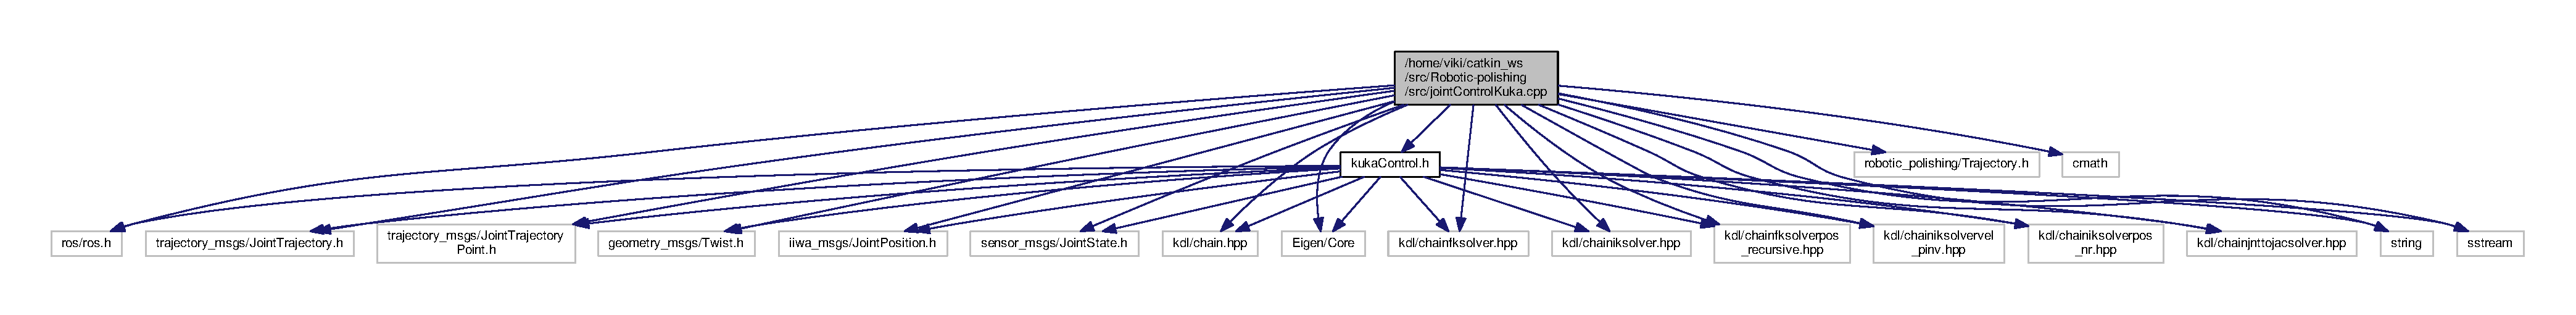
\includegraphics[width=350pt]{jointControlKuka_8cpp__incl}
\end{center}
\end{figure}
\subsection*{Classes}
\begin{DoxyCompactItemize}
\item 
struct \hyperlink{structposition}{position}
\end{DoxyCompactItemize}
\subsection*{Functions}
\begin{DoxyCompactItemize}
\item 
void \hyperlink{jointControlKuka_8cpp_a1252494bba2bc971fdb228ed8330f08d}{get\+\_\+joints} (const sensor\+\_\+msgs\+::\+Joint\+State \&data)
\begin{DoxyCompactList}\small\item\em get\+\_\+joints is a callback function that subscribe the joint position data and set it into joints vector \end{DoxyCompactList}\item 
int {\bfseries main} (int argc, char $\ast$argv\mbox{[}$\,$\mbox{]})\hypertarget{jointControlKuka_8cpp_a0ddf1224851353fc92bfbff6f499fa97}{}\label{jointControlKuka_8cpp_a0ddf1224851353fc92bfbff6f499fa97}

\end{DoxyCompactItemize}
\subsection*{Variables}
\begin{DoxyCompactItemize}
\item 
sensor\+\_\+msgs\+::\+Joint\+State {\bfseries joints}\hypertarget{jointControlKuka_8cpp_ae1f6b7f93d34b40bafa1e4773a663acb}{}\label{jointControlKuka_8cpp_ae1f6b7f93d34b40bafa1e4773a663acb}

\item 
bool {\bfseries initialized} = false\hypertarget{jointControlKuka_8cpp_aedeffc7d23da25d52b9a50045189fe2b}{}\label{jointControlKuka_8cpp_aedeffc7d23da25d52b9a50045189fe2b}

\item 
double {\bfseries threshold} = 0.\+005\hypertarget{jointControlKuka_8cpp_afcfbedec6ebde62c6a091ce335836ef1}{}\label{jointControlKuka_8cpp_afcfbedec6ebde62c6a091ce335836ef1}

\item 
struct \hyperlink{structposition}{position} {\bfseries test1}\hypertarget{jointControlKuka_8cpp_a4c12048046fc75dd88e1da048f21857d}{}\label{jointControlKuka_8cpp_a4c12048046fc75dd88e1da048f21857d}

\end{DoxyCompactItemize}


\subsection{Detailed Description}
This \hyperlink{jointControlKuka_8cpp}{joint\+Control\+Kuka.\+cpp} is a ros node that use to control the iiwa in gazebo. 

\begin{DoxyAuthor}{Author}
Michael Kam (michael081906) 
\end{DoxyAuthor}
\begin{DoxyRefDesc}{Bug}
\item[\hyperlink{bug__bug000023}{Bug}]No known bugs. \end{DoxyRefDesc}
\begin{DoxyCopyright}{Copyright}
G\+NU Public License.
\end{DoxyCopyright}
joint\+Control\+Kuka is free software\+: you can redistribute it and/or modify it under the terms of the G\+NU General Public License as published by the Free Software Foundation, either version 3 of the License, or (at your option) any later version.

joint\+Control\+Kuka is distributed in the hope that it will be useful, but W\+I\+T\+H\+O\+UT A\+NY W\+A\+R\+R\+A\+N\+TY; without even the implied warranty of M\+E\+R\+C\+H\+A\+N\+T\+A\+B\+I\+L\+I\+TY or F\+I\+T\+N\+E\+SS F\+OR A P\+A\+R\+T\+I\+C\+U\+L\+AR P\+U\+R\+P\+O\+SE. See the G\+NU General Public License for more details. You should have received a copy of the G\+NU General Public License along with joint\+Control\+Kuka. If not, see \href{http://www.gnu.org/licenses/}{\tt http\+://www.\+gnu.\+org/licenses/}. 

\subsection{Function Documentation}
\index{joint\+Control\+Kuka.\+cpp@{joint\+Control\+Kuka.\+cpp}!get\+\_\+joints@{get\+\_\+joints}}
\index{get\+\_\+joints@{get\+\_\+joints}!joint\+Control\+Kuka.\+cpp@{joint\+Control\+Kuka.\+cpp}}
\subsubsection[{\texorpdfstring{get\+\_\+joints(const sensor\+\_\+msgs\+::\+Joint\+State \&data)}{get_joints(const sensor_msgs::JointState &data)}}]{\setlength{\rightskip}{0pt plus 5cm}void get\+\_\+joints (
\begin{DoxyParamCaption}
\item[{const sensor\+\_\+msgs\+::\+Joint\+State \&}]{data}
\end{DoxyParamCaption}
)}\hypertarget{jointControlKuka_8cpp_a1252494bba2bc971fdb228ed8330f08d}{}\label{jointControlKuka_8cpp_a1252494bba2bc971fdb228ed8330f08d}


get\+\_\+joints is a callback function that subscribe the joint position data and set it into joints vector 


\begin{DoxyParams}[1]{Parameters}
\mbox{\tt in}  & {\em data} & sensor\+\_\+msgs\+::\+Joint\+State that contains joint position \\
\hline
\end{DoxyParams}
\begin{DoxyReturn}{Returns}
none 
\end{DoxyReturn}

\hypertarget{kukaControl_8cpp}{}\section{/home/viki/catkin\+\_\+ws/src/\+Robotic-\/polishing/src/kuka\+\_\+control/kuka\+Control.cpp File Reference}
\label{kukaControl_8cpp}\index{/home/viki/catkin\+\_\+ws/src/\+Robotic-\/polishing/src/kuka\+\_\+control/kuka\+Control.\+cpp@{/home/viki/catkin\+\_\+ws/src/\+Robotic-\/polishing/src/kuka\+\_\+control/kuka\+Control.\+cpp}}


This \hyperlink{kukaControl_8cpp}{kuka\+Control.\+cpp} is an implement file of controlling the iiwa kuka arm.  


{\ttfamily \#include \char`\"{}kuka\+Control.\+h\char`\"{}}\\*
{\ttfamily \#include $<$ros/ros.\+h$>$}\\*
{\ttfamily \#include $<$trajectory\+\_\+msgs/\+Joint\+Trajectory.\+h$>$}\\*
{\ttfamily \#include $<$trajectory\+\_\+msgs/\+Joint\+Trajectory\+Point.\+h$>$}\\*
{\ttfamily \#include $<$geometry\+\_\+msgs/\+Twist.\+h$>$}\\*
{\ttfamily \#include $<$iiwa\+\_\+msgs/\+Joint\+Position.\+h$>$}\\*
{\ttfamily \#include $<$sensor\+\_\+msgs/\+Joint\+State.\+h$>$}\\*
{\ttfamily \#include $<$kdl/chain.\+hpp$>$}\\*
{\ttfamily \#include \char`\"{}Eigen/\+Core\char`\"{}}\\*
{\ttfamily \#include $<$kdl/chainfksolver.\+hpp$>$}\\*
{\ttfamily \#include $<$kdl/chainiksolver.\+hpp$>$}\\*
{\ttfamily \#include $<$kdl/chainfksolverpos\+\_\+recursive.\+hpp$>$}\\*
{\ttfamily \#include $<$kdl/chainiksolvervel\+\_\+pinv.\+hpp$>$}\\*
{\ttfamily \#include $<$kdl/chainiksolverpos\+\_\+nr.\+hpp$>$}\\*
{\ttfamily \#include $<$kdl/chainjnttojacsolver.\+hpp$>$}\\*
{\ttfamily \#include $<$string$>$}\\*
{\ttfamily \#include $<$sstream$>$}\\*
Include dependency graph for kuka\+Control.\+cpp\+:
\nopagebreak
\begin{figure}[H]
\begin{center}
\leavevmode
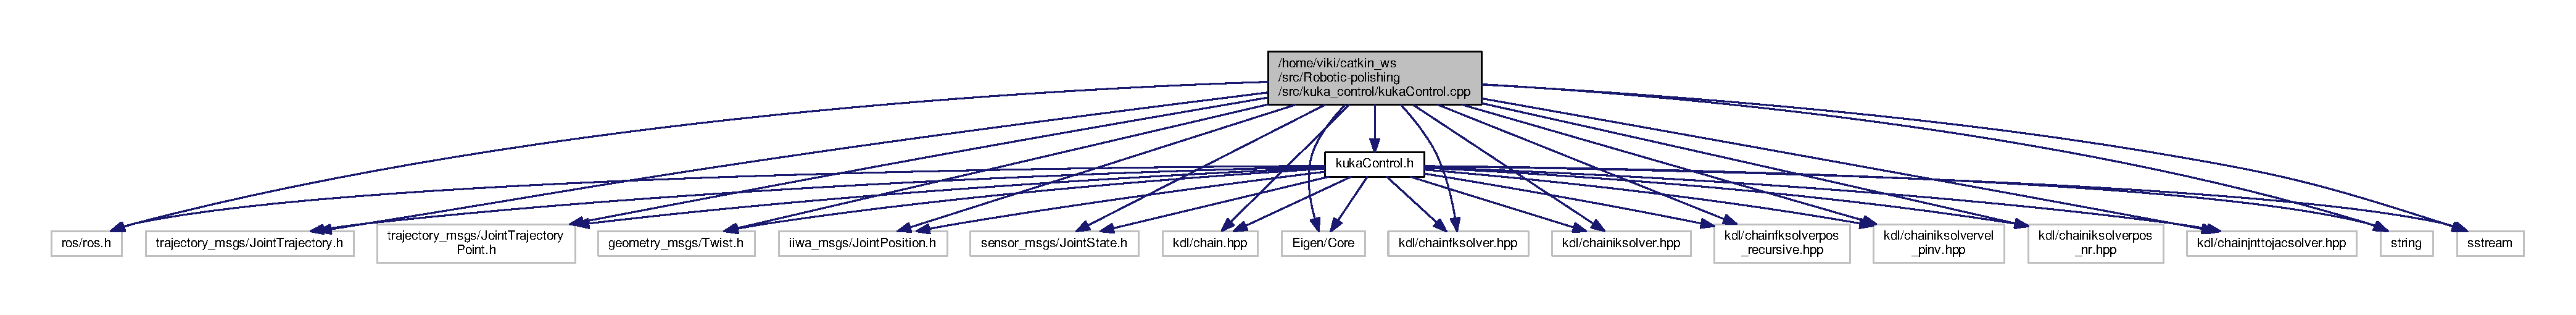
\includegraphics[width=350pt]{kukaControl_8cpp__incl}
\end{center}
\end{figure}


\subsection{Detailed Description}
This \hyperlink{kukaControl_8cpp}{kuka\+Control.\+cpp} is an implement file of controlling the iiwa kuka arm. 

\begin{DoxyAuthor}{Author}
Michael Kam (michael081906) 
\end{DoxyAuthor}
\begin{DoxyRefDesc}{Bug}
\item[\hyperlink{bug__bug000025}{Bug}]No known bugs. \end{DoxyRefDesc}
\begin{DoxyCopyright}{Copyright}
G\+NU Public License.
\end{DoxyCopyright}
\hyperlink{classkukaControl}{kuka\+Control} is free software\+: you can redistribute it and/or modify it under the terms of the G\+NU General Public License as published by the Free Software Foundation, either version 3 of the License, or (at your option) any later version.

\hyperlink{classkukaControl}{kuka\+Control} is distributed in the hope that it will be useful, but W\+I\+T\+H\+O\+UT A\+NY W\+A\+R\+R\+A\+N\+TY; without even the implied warranty of M\+E\+R\+C\+H\+A\+N\+T\+A\+B\+I\+L\+I\+TY or F\+I\+T\+N\+E\+SS F\+OR A P\+A\+R\+T\+I\+C\+U\+L\+AR P\+U\+R\+P\+O\+SE. See the G\+NU General Public License for more details. You should have received a copy of the G\+NU General Public License along with \hyperlink{classkukaControl}{kuka\+Control}. If not, see \href{http://www.gnu.org/licenses/}{\tt http\+://www.\+gnu.\+org/licenses/}. 
\hypertarget{dijkstraPQ_8cpp}{}\section{/home/viki/catkin\+\_\+ws/src/\+Robotic-\/polishing/src/pcl\+\_\+midterm/dijkstra\+PQ.cpp File Reference}
\label{dijkstraPQ_8cpp}\index{/home/viki/catkin\+\_\+ws/src/\+Robotic-\/polishing/src/pcl\+\_\+midterm/dijkstra\+P\+Q.\+cpp@{/home/viki/catkin\+\_\+ws/src/\+Robotic-\/polishing/src/pcl\+\_\+midterm/dijkstra\+P\+Q.\+cpp}}


This \hyperlink{dijkstraPQ_8cpp}{dijkstra\+P\+Q.\+cpp} is an implementation of finding shortest path among the point cloud. The algorithm refer to here\+: \href{http://www.geeksforgeeks.org/dijkstras-shortest-path-algorithm-using-priority_queue-stl/}{\tt http\+://www.\+geeksforgeeks.\+org/dijkstras-\/shortest-\/path-\/algorithm-\/using-\/priority\+\_\+queue-\/stl/}.  


{\ttfamily \#include \char`\"{}dijkstra\+P\+Q.\+h\char`\"{}}\\*
{\ttfamily \#include $<$bits/stdc++.\+h$>$}\\*
Include dependency graph for dijkstra\+P\+Q.\+cpp\+:
\nopagebreak
\begin{figure}[H]
\begin{center}
\leavevmode
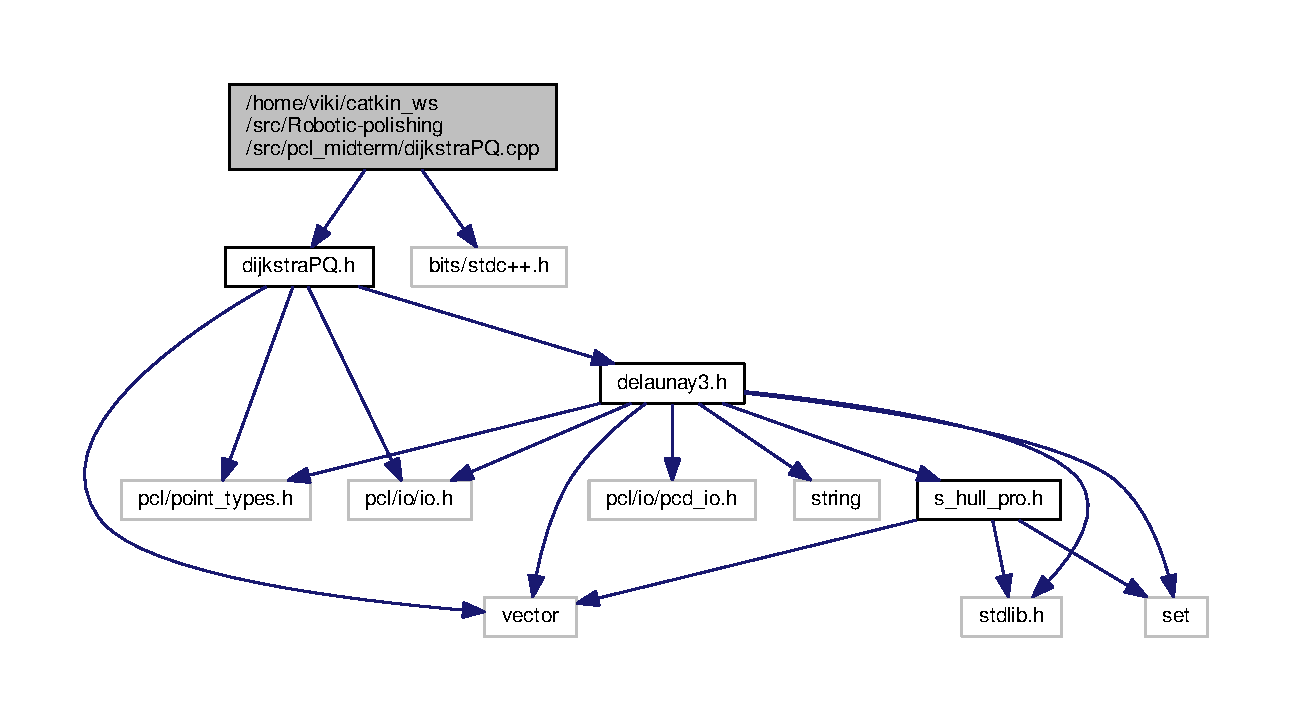
\includegraphics[width=350pt]{dijkstraPQ_8cpp__incl}
\end{center}
\end{figure}
\subsection*{Macros}
\begin{DoxyCompactItemize}
\item 
\#define {\bfseries I\+NF}~0x3f3f3f3f\hypertarget{dijkstraPQ_8cpp_a12c2040f25d8e3a7b9e1c2024c618cb6}{}\label{dijkstraPQ_8cpp_a12c2040f25d8e3a7b9e1c2024c618cb6}

\end{DoxyCompactItemize}


\subsection{Detailed Description}
This \hyperlink{dijkstraPQ_8cpp}{dijkstra\+P\+Q.\+cpp} is an implementation of finding shortest path among the point cloud. The algorithm refer to here\+: \href{http://www.geeksforgeeks.org/dijkstras-shortest-path-algorithm-using-priority_queue-stl/}{\tt http\+://www.\+geeksforgeeks.\+org/dijkstras-\/shortest-\/path-\/algorithm-\/using-\/priority\+\_\+queue-\/stl/}. 

\begin{DoxyAuthor}{Author}
Michael Kam (michael081906) 
\end{DoxyAuthor}
\begin{DoxyRefDesc}{Bug}
\item[\hyperlink{bug__bug000027}{Bug}]No known bugs. \end{DoxyRefDesc}
\begin{DoxyCopyright}{Copyright}
G\+NU Public License.
\end{DoxyCopyright}
\hyperlink{classdijkstraPQ}{dijkstra\+PQ} is free software\+: you can redistribute it and/or modify it under the terms of the G\+NU General Public License as published by the Free Software Foundation, either version 3 of the License, or (at your option) any later version.

\hyperlink{classdijkstraPQ}{dijkstra\+PQ} is distributed in the hope that it will be useful, but W\+I\+T\+H\+O\+UT A\+NY W\+A\+R\+R\+A\+N\+TY; without even the implied warranty of M\+E\+R\+C\+H\+A\+N\+T\+A\+B\+I\+L\+I\+TY or F\+I\+T\+N\+E\+SS F\+OR A P\+A\+R\+T\+I\+C\+U\+L\+AR P\+U\+R\+P\+O\+SE. See the G\+NU General Public License for more details. You should have received a copy of the G\+NU General Public License along with \hyperlink{classdijkstraPQ}{dijkstra\+PQ}. If not, see \href{http://www.gnu.org/licenses/}{\tt http\+://www.\+gnu.\+org/licenses/}. 
\hypertarget{findNearestPoint_8cpp}{}\section{/home/viki/catkin\+\_\+ws/src/\+Robotic-\/polishing/src/pcl\+\_\+midterm/find\+Nearest\+Point.cpp File Reference}
\label{findNearestPoint_8cpp}\index{/home/viki/catkin\+\_\+ws/src/\+Robotic-\/polishing/src/pcl\+\_\+midterm/find\+Nearest\+Point.\+cpp@{/home/viki/catkin\+\_\+ws/src/\+Robotic-\/polishing/src/pcl\+\_\+midterm/find\+Nearest\+Point.\+cpp}}


This \hyperlink{findNearestPoint_8h_source}{find\+Nearest\+Point.\+h} is a header file of finding the closest point on a post smoothing surface. There are three method in this class. The goal is to get indices array which indicate the closest point with several given points. For example, I can given a arbitrary coordinate and use this class to find a closest point ID from point cloud group.  


{\ttfamily \#include $<$find\+Nearest\+Point.\+h$>$}\\*
{\ttfamily \#include $<$stdlib.\+h$>$}\\*
{\ttfamily \#include $<$pcl/point\+\_\+cloud.\+h$>$}\\*
{\ttfamily \#include $<$pcl/kdtree/kdtree\+\_\+flann.\+h$>$}\\*
{\ttfamily \#include $<$iostream$>$}\\*
{\ttfamily \#include $<$string$>$}\\*
{\ttfamily \#include $<$fstream$>$}\\*
{\ttfamily \#include $<$vector$>$}\\*
{\ttfamily \#include $<$ctime$>$}\\*
Include dependency graph for find\+Nearest\+Point.\+cpp\+:
\nopagebreak
\begin{figure}[H]
\begin{center}
\leavevmode
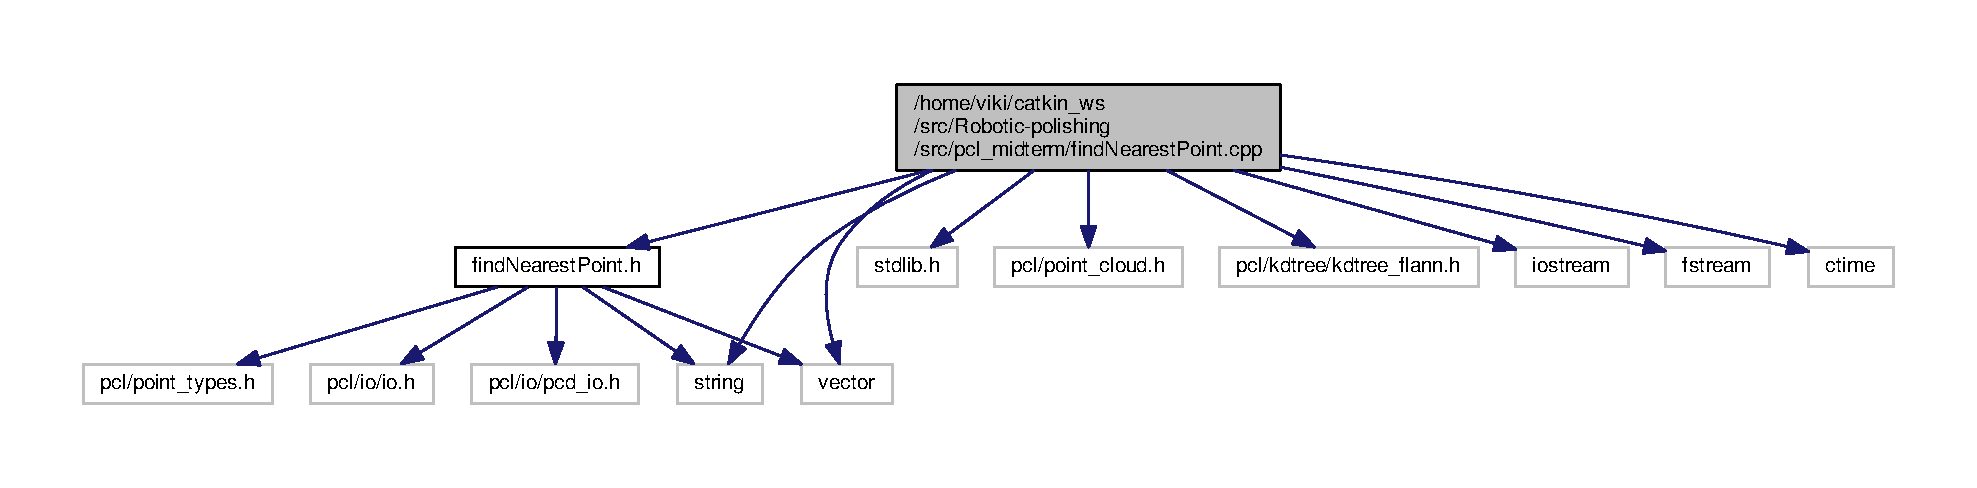
\includegraphics[width=350pt]{findNearestPoint_8cpp__incl}
\end{center}
\end{figure}


\subsection{Detailed Description}
This \hyperlink{findNearestPoint_8h_source}{find\+Nearest\+Point.\+h} is a header file of finding the closest point on a post smoothing surface. There are three method in this class. The goal is to get indices array which indicate the closest point with several given points. For example, I can given a arbitrary coordinate and use this class to find a closest point ID from point cloud group. 

This \hyperlink{findNearestPoint_8cpp}{find\+Nearest\+Point.\+cpp} is an implementation of finding the closest point on a post smoothing surface. There are three method in this class. The goal is to get indices array which indicate the closest point with several given points. For example, I can given a arbitrary coordinate and use this class to find a closest point ID from point cloud group.

\begin{DoxyAuthor}{Author}
Michael Kam (michael081906) 
\end{DoxyAuthor}
\begin{DoxyRefDesc}{Bug}
\item[\hyperlink{bug__bug000005}{Bug}]No known bugs. \end{DoxyRefDesc}
\begin{DoxyCopyright}{Copyright}
G\+NU Public License.
\end{DoxyCopyright}
\hyperlink{classfindNearestPoint}{find\+Nearest\+Point} is free software\+: you can redistribute it and/or modify it under the terms of the G\+NU General Public License as published by the Free Software Foundation, either version 3 of the License, or (at your option) any later version.

\hyperlink{classfindNearestPoint}{find\+Nearest\+Point} is distributed in the hope that it will be useful, but W\+I\+T\+H\+O\+UT A\+NY W\+A\+R\+R\+A\+N\+TY; without even the implied warranty of M\+E\+R\+C\+H\+A\+N\+T\+A\+B\+I\+L\+I\+TY or F\+I\+T\+N\+E\+SS F\+OR A P\+A\+R\+T\+I\+C\+U\+L\+AR P\+U\+R\+P\+O\+SE. See the G\+NU General Public License for more details. You should have received a copy of the G\+NU General Public License along with \hyperlink{classfindNearestPoint}{find\+Nearest\+Point}. If not, see \href{http://www.gnu.org/licenses/}{\tt http\+://www.\+gnu.\+org/licenses/}.

\begin{DoxyAuthor}{Author}
Michael Kam (michael081906) 
\end{DoxyAuthor}
\begin{DoxyRefDesc}{Bug}
\item[\hyperlink{bug__bug000028}{Bug}]No known bugs. \end{DoxyRefDesc}
\begin{DoxyCopyright}{Copyright}
G\+NU Public License.
\end{DoxyCopyright}
\hyperlink{classfindNearestPoint}{find\+Nearest\+Point} is free software\+: you can redistribute it and/or modify it under the terms of the G\+NU General Public License as published by the Free Software Foundation, either version 3 of the License, or (at your option) any later version.

\hyperlink{classfindNearestPoint}{find\+Nearest\+Point} is distributed in the hope that it will be useful, but W\+I\+T\+H\+O\+UT A\+NY W\+A\+R\+R\+A\+N\+TY; without even the implied warranty of M\+E\+R\+C\+H\+A\+N\+T\+A\+B\+I\+L\+I\+TY or F\+I\+T\+N\+E\+SS F\+OR A P\+A\+R\+T\+I\+C\+U\+L\+AR P\+U\+R\+P\+O\+SE. See the G\+NU General Public License for more details. You should have received a copy of the G\+NU General Public License along with \hyperlink{classfindNearestPoint}{find\+Nearest\+Point}. If not, see \href{http://www.gnu.org/licenses/}{\tt http\+://www.\+gnu.\+org/licenses/}. 
\hypertarget{pclCloudViewer_8cpp}{}\section{/home/viki/catkin\+\_\+ws/src/\+Robotic-\/polishing/src/pcl\+\_\+midterm/pcl\+Cloud\+Viewer.cpp File Reference}
\label{pclCloudViewer_8cpp}\index{/home/viki/catkin\+\_\+ws/src/\+Robotic-\/polishing/src/pcl\+\_\+midterm/pcl\+Cloud\+Viewer.\+cpp@{/home/viki/catkin\+\_\+ws/src/\+Robotic-\/polishing/src/pcl\+\_\+midterm/pcl\+Cloud\+Viewer.\+cpp}}


This is the implementation of the \hyperlink{classpclCloudViewer}{pcl\+Cloud\+Viewer} class. This class consists of 1 method. Please refer the \hyperlink{pclCloudViewer_8h}{pcl\+Cloud\+Viewer.\+h} for more detail.  


{\ttfamily \#include $<$pcl/visualization/cloud\+\_\+viewer.\+h$>$}\\*
{\ttfamily \#include $<$pcl/io/io.\+h$>$}\\*
{\ttfamily \#include $<$pcl/io/pcd\+\_\+io.\+h$>$}\\*
{\ttfamily \#include $<$pcl/point\+\_\+types.\+h$>$}\\*
{\ttfamily \#include \char`\"{}pcl\+Cloud\+Viewer.\+h\char`\"{}}\\*
{\ttfamily \#include $<$iostream$>$}\\*
Include dependency graph for pcl\+Cloud\+Viewer.\+cpp\+:
\nopagebreak
\begin{figure}[H]
\begin{center}
\leavevmode
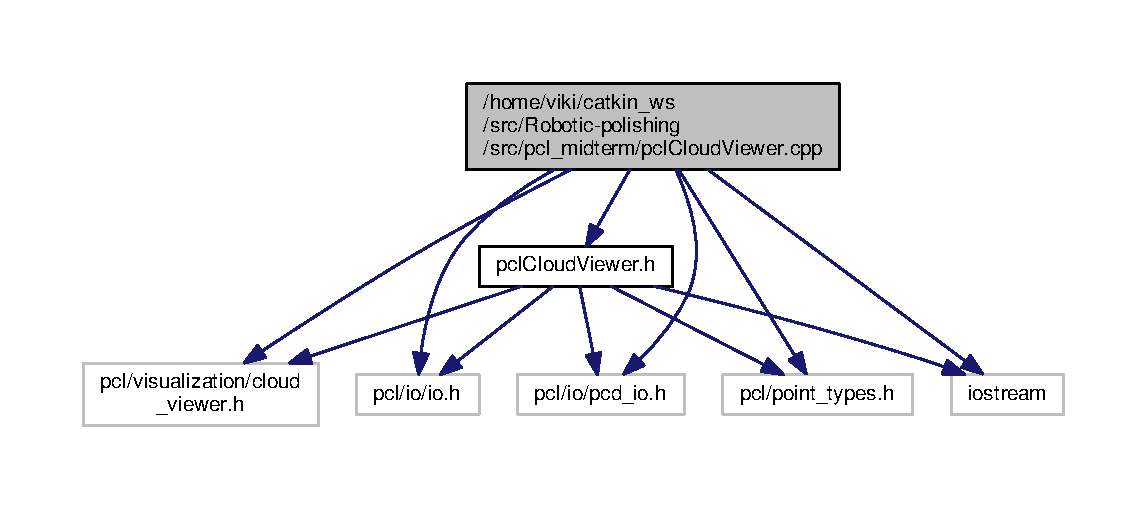
\includegraphics[width=350pt]{pclCloudViewer_8cpp__incl}
\end{center}
\end{figure}


\subsection{Detailed Description}
This is the implementation of the \hyperlink{classpclCloudViewer}{pcl\+Cloud\+Viewer} class. This class consists of 1 method. Please refer the \hyperlink{pclCloudViewer_8h}{pcl\+Cloud\+Viewer.\+h} for more detail. 

\begin{DoxyAuthor}{Author}
Michael Kam (michael081906) 
\end{DoxyAuthor}
\begin{DoxyRefDesc}{Bug}
\item[\hyperlink{bug__bug000029}{Bug}]No known bugs. \end{DoxyRefDesc}
\begin{DoxyCopyright}{Copyright}
G\+NU Public License.
\end{DoxyCopyright}
This class utilize pcl visualization to display point cloud.

\begin{DoxyAuthor}{Author}
Michael Kam (michael081906) 
\end{DoxyAuthor}
\begin{DoxyRefDesc}{Bug}
\item[\hyperlink{bug__bug000030}{Bug}]No1 can\textquotesingle{}t not be compile successfully in the test case. \end{DoxyRefDesc}
\begin{DoxyCopyright}{Copyright}
G\+NU Public License.
\end{DoxyCopyright}
\hyperlink{classpclCloudViewer}{pcl\+Cloud\+Viewer} is free software\+: you can redistribute it and/or modify it under the terms of the G\+NU General Public License as published by the Free Software Foundation, either version 3 of the License, or (at your option) any later version.

\hyperlink{classpclCloudViewer}{pcl\+Cloud\+Viewer} is distributed in the hope that it will be useful, but W\+I\+T\+H\+O\+UT A\+NY W\+A\+R\+R\+A\+N\+TY; without even the implied warranty of M\+E\+R\+C\+H\+A\+N\+T\+A\+B\+I\+L\+I\+TY or F\+I\+T\+N\+E\+SS F\+OR A P\+A\+R\+T\+I\+C\+U\+L\+AR P\+U\+R\+P\+O\+SE. See the G\+NU General Public License for more details. You should have received a copy of the G\+NU General Public License along with \hyperlink{classpclCloudViewer}{pcl\+Cloud\+Viewer}. If not, see \href{http://www.gnu.org/licenses/}{\tt http\+://www.\+gnu.\+org/licenses/}. $\ast$ 
\hypertarget{pclFastTriangular_8cpp}{}\section{/home/viki/catkin\+\_\+ws/src/\+Robotic-\/polishing/src/pcl\+\_\+midterm/pcl\+Fast\+Triangular.cpp File Reference}
\label{pclFastTriangular_8cpp}\index{/home/viki/catkin\+\_\+ws/src/\+Robotic-\/polishing/src/pcl\+\_\+midterm/pcl\+Fast\+Triangular.\+cpp@{/home/viki/catkin\+\_\+ws/src/\+Robotic-\/polishing/src/pcl\+\_\+midterm/pcl\+Fast\+Triangular.\+cpp}}


This is the implementation of the \hyperlink{classpclFastTriangular}{pcl\+Fast\+Triangular} class. This class consists of 6 methods. Please refer the \hyperlink{pclFastTriangular_8h}{pcl\+Fast\+Triangular.\+h} for more detail.  


{\ttfamily \#include $<$pcl/io/io.\+h$>$}\\*
{\ttfamily \#include $<$pcl/io/pcd\+\_\+io.\+h$>$}\\*
{\ttfamily \#include $<$pcl/point\+\_\+types.\+h$>$}\\*
{\ttfamily \#include $<$pcl/kdtree/kdtree\+\_\+flann.\+h$>$}\\*
{\ttfamily \#include $<$pcl/features/normal\+\_\+3d.\+h$>$}\\*
{\ttfamily \#include $<$pcl/surface/gp3.\+h$>$}\\*
{\ttfamily \#include $<$pcl\+Fast\+Triangular.\+h$>$}\\*
{\ttfamily \#include $<$ios$>$}\\*
{\ttfamily \#include $<$vector$>$}\\*
{\ttfamily \#include $<$iostream$>$}\\*
Include dependency graph for pcl\+Fast\+Triangular.\+cpp\+:
\nopagebreak
\begin{figure}[H]
\begin{center}
\leavevmode
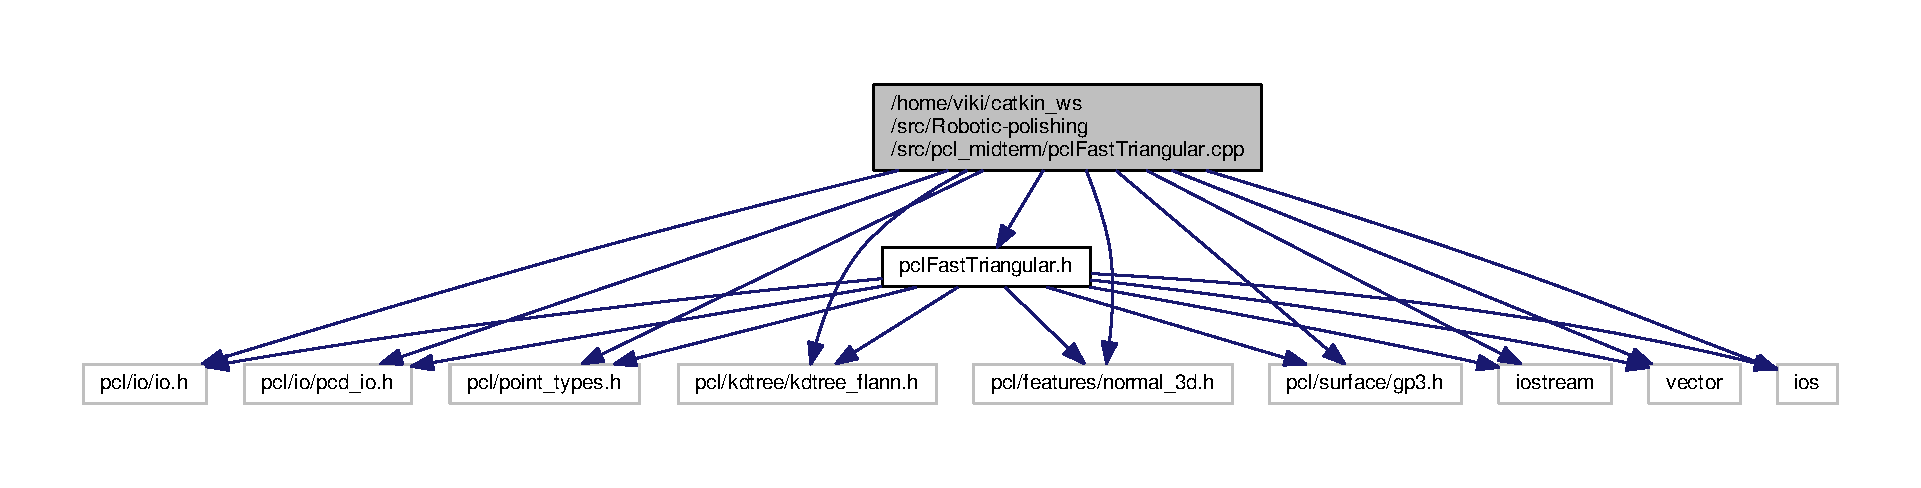
\includegraphics[width=350pt]{pclFastTriangular_8cpp__incl}
\end{center}
\end{figure}


\subsection{Detailed Description}
This is the implementation of the \hyperlink{classpclFastTriangular}{pcl\+Fast\+Triangular} class. This class consists of 6 methods. Please refer the \hyperlink{pclFastTriangular_8h}{pcl\+Fast\+Triangular.\+h} for more detail. 

\begin{DoxyAuthor}{Author}
Michael Kam (michael081906) 
\end{DoxyAuthor}
\begin{DoxyRefDesc}{Bug}
\item[\hyperlink{bug__bug000031}{Bug}]No known bugs. \end{DoxyRefDesc}
\begin{DoxyCopyright}{Copyright}
G\+NU Public License.
\end{DoxyCopyright}
\hyperlink{classpclFastTriangular}{pcl\+Fast\+Triangular} is free software\+: you can redistribute it and/or modify it under the terms of the G\+NU General Public License as published by the Free Software Foundation, either version 3 of the License, or (at your option) any later version.

\hyperlink{classpclFastTriangular}{pcl\+Fast\+Triangular} is distributed in the hope that it will be useful, but W\+I\+T\+H\+O\+UT A\+NY W\+A\+R\+R\+A\+N\+TY; without even the implied warranty of M\+E\+R\+C\+H\+A\+N\+T\+A\+B\+I\+L\+I\+TY or F\+I\+T\+N\+E\+SS F\+OR A P\+A\+R\+T\+I\+C\+U\+L\+AR P\+U\+R\+P\+O\+SE. See the G\+NU General Public License for more details. You should have received a copy of the G\+NU General Public License along with \hyperlink{classpclFastTriangular}{pcl\+Fast\+Triangular}. If not, see \href{http://www.gnu.org/licenses/}{\tt http\+://www.\+gnu.\+org/licenses/}. 
\hypertarget{pclIo_8cpp}{}\section{/home/viki/catkin\+\_\+ws/src/\+Robotic-\/polishing/src/pcl\+\_\+midterm/pcl\+Io.cpp File Reference}
\label{pclIo_8cpp}\index{/home/viki/catkin\+\_\+ws/src/\+Robotic-\/polishing/src/pcl\+\_\+midterm/pcl\+Io.\+cpp@{/home/viki/catkin\+\_\+ws/src/\+Robotic-\/polishing/src/pcl\+\_\+midterm/pcl\+Io.\+cpp}}


This is the implementation of the \hyperlink{classpclIo}{pcl\+Io} class. This class consists of 2 methods. Please refer the \hyperlink{pclIo_8h}{pcl\+Io.\+h} for more detail.  


{\ttfamily \#include \char`\"{}pcl\+Io.\+h\char`\"{}}\\*
{\ttfamily \#include $<$pcl/io/pcd\+\_\+io.\+h$>$}\\*
{\ttfamily \#include $<$pcl/point\+\_\+types.\+h$>$}\\*
{\ttfamily \#include $<$iostream$>$}\\*
{\ttfamily \#include $<$string$>$}\\*
Include dependency graph for pcl\+Io.\+cpp\+:
\nopagebreak
\begin{figure}[H]
\begin{center}
\leavevmode
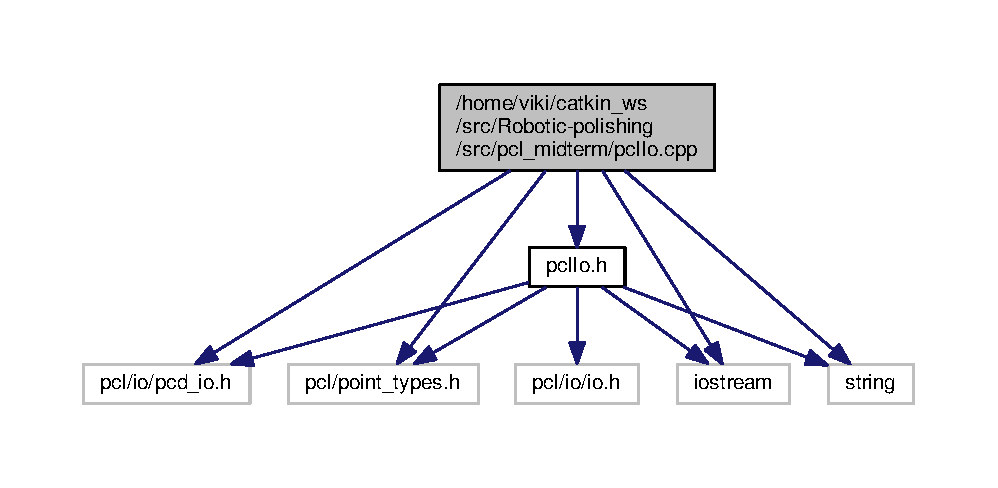
\includegraphics[width=350pt]{pclIo_8cpp__incl}
\end{center}
\end{figure}


\subsection{Detailed Description}
This is the implementation of the \hyperlink{classpclIo}{pcl\+Io} class. This class consists of 2 methods. Please refer the \hyperlink{pclIo_8h}{pcl\+Io.\+h} for more detail. 

\begin{DoxyAuthor}{Author}
Michael Kam (michael081906) 
\end{DoxyAuthor}
\begin{DoxyRefDesc}{Bug}
\item[\hyperlink{bug__bug000032}{Bug}]No known bugs. \end{DoxyRefDesc}
\begin{DoxyCopyright}{Copyright}
G\+NU Public License.
\end{DoxyCopyright}
\hyperlink{classpclIo}{pcl\+Io} is free software\+: you can redistribute it and/or modify it under the terms of the G\+NU General Public License as published by the Free Software Foundation, either version 3 of the License, or (at your option) any later version.

\hyperlink{classpclIo}{pcl\+Io} is distributed in the hope that it will be useful, but W\+I\+T\+H\+O\+UT A\+NY W\+A\+R\+R\+A\+N\+TY; without even the implied warranty of M\+E\+R\+C\+H\+A\+N\+T\+A\+B\+I\+L\+I\+TY or F\+I\+T\+N\+E\+SS F\+OR A P\+A\+R\+T\+I\+C\+U\+L\+AR P\+U\+R\+P\+O\+SE. See the G\+NU General Public License for more details. You should have received a copy of the G\+NU General Public License along with \hyperlink{classpclIo}{pcl\+Io}. If not, see \href{http://www.gnu.org/licenses/}{\tt http\+://www.\+gnu.\+org/licenses/}. 
\hypertarget{pclMlsSmoothing_8cpp}{}\section{/home/viki/catkin\+\_\+ws/src/\+Robotic-\/polishing/src/pcl\+\_\+midterm/pcl\+Mls\+Smoothing.cpp File Reference}
\label{pclMlsSmoothing_8cpp}\index{/home/viki/catkin\+\_\+ws/src/\+Robotic-\/polishing/src/pcl\+\_\+midterm/pcl\+Mls\+Smoothing.\+cpp@{/home/viki/catkin\+\_\+ws/src/\+Robotic-\/polishing/src/pcl\+\_\+midterm/pcl\+Mls\+Smoothing.\+cpp}}


This is the implementation of the \hyperlink{classpclMlsSmoothing}{pcl\+Mls\+Smoothing} class. This class consists of 5 methods. Please refer the \hyperlink{pclMlsSmoothing_8h}{pcl\+Mls\+Smoothing.\+h} for more detail.  


{\ttfamily \#include $<$pcl/io/io.\+h$>$}\\*
{\ttfamily \#include $<$pcl/io/pcd\+\_\+io.\+h$>$}\\*
{\ttfamily \#include $<$pcl/point\+\_\+types.\+h$>$}\\*
{\ttfamily \#include $<$pcl\+Mls\+Smoothing.\+h$>$}\\*
{\ttfamily \#include $<$ios$>$}\\*
{\ttfamily \#include $<$iostream$>$}\\*
Include dependency graph for pcl\+Mls\+Smoothing.\+cpp\+:
\nopagebreak
\begin{figure}[H]
\begin{center}
\leavevmode
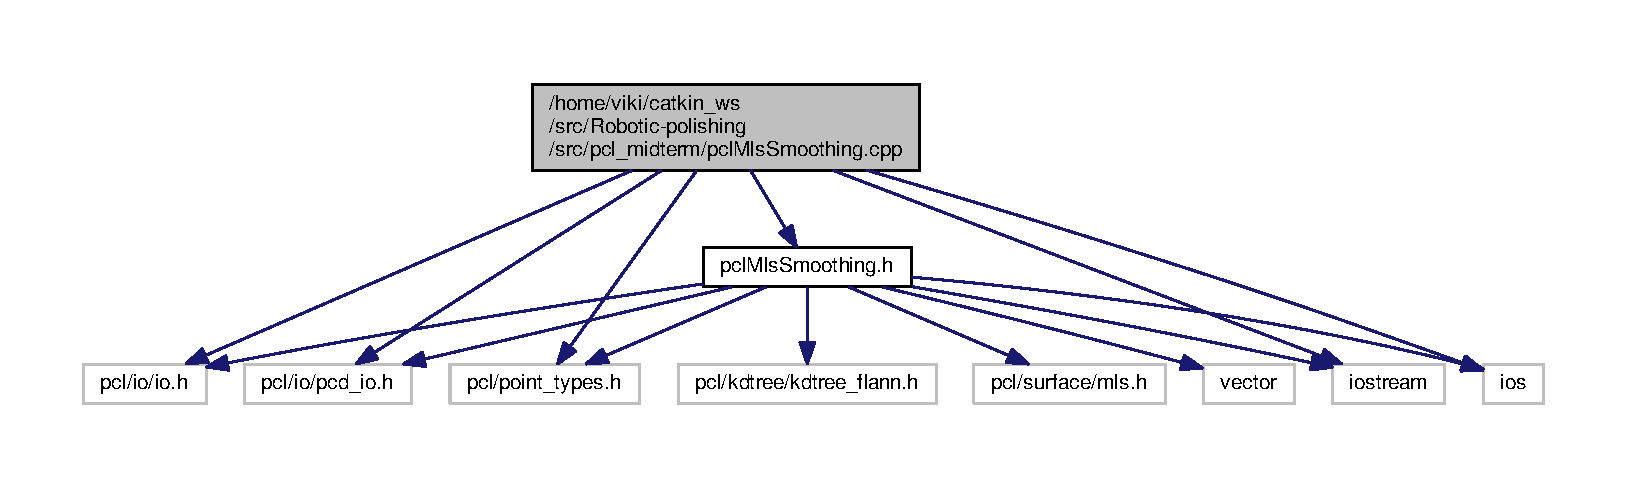
\includegraphics[width=350pt]{pclMlsSmoothing_8cpp__incl}
\end{center}
\end{figure}


\subsection{Detailed Description}
This is the implementation of the \hyperlink{classpclMlsSmoothing}{pcl\+Mls\+Smoothing} class. This class consists of 5 methods. Please refer the \hyperlink{pclMlsSmoothing_8h}{pcl\+Mls\+Smoothing.\+h} for more detail. 

\begin{DoxyAuthor}{Author}
Michael Kam (michael081906) 
\end{DoxyAuthor}
\begin{DoxyRefDesc}{Bug}
\item[\hyperlink{bug__bug000033}{Bug}]No known bugs. \end{DoxyRefDesc}
\begin{DoxyCopyright}{Copyright}
G\+NU Public License.
\end{DoxyCopyright}
\hyperlink{classpclMlsSmoothing}{pcl\+Mls\+Smoothing} is free software\+: you can redistribute it and/or modify it under the terms of the G\+NU General Public License as published by the Free Software Foundation, either version 3 of the License, or (at your option) any later version.

\hyperlink{classpclMlsSmoothing}{pcl\+Mls\+Smoothing} is distributed in the hope that it will be useful, but W\+I\+T\+H\+O\+UT A\+NY W\+A\+R\+R\+A\+N\+TY; without even the implied warranty of M\+E\+R\+C\+H\+A\+N\+T\+A\+B\+I\+L\+I\+TY or F\+I\+T\+N\+E\+SS F\+OR A P\+A\+R\+T\+I\+C\+U\+L\+AR P\+U\+R\+P\+O\+SE. See the G\+NU General Public License for more details. You should have received a copy of the G\+NU General Public License along with \hyperlink{classpclMlsSmoothing}{pcl\+Mls\+Smoothing}. If not, see \href{http://www.gnu.org/licenses/}{\tt http\+://www.\+gnu.\+org/licenses/}. 
\hypertarget{pclPassThrough_8cpp}{}\section{/home/viki/catkin\+\_\+ws/src/\+Robotic-\/polishing/src/pcl\+\_\+midterm/pcl\+Pass\+Through.cpp File Reference}
\label{pclPassThrough_8cpp}\index{/home/viki/catkin\+\_\+ws/src/\+Robotic-\/polishing/src/pcl\+\_\+midterm/pcl\+Pass\+Through.\+cpp@{/home/viki/catkin\+\_\+ws/src/\+Robotic-\/polishing/src/pcl\+\_\+midterm/pcl\+Pass\+Through.\+cpp}}


This is the implementation of the \hyperlink{classpclPassThrough}{pcl\+Pass\+Through} class. This class consists of 7 methods. Please refer the \hyperlink{pclPassThrough_8h_source}{pcl\+Pass\+Through.\+h} for more detail.  


{\ttfamily \#include $<$pcl/io/io.\+h$>$}\\*
{\ttfamily \#include $<$pcl/io/pcd\+\_\+io.\+h$>$}\\*
{\ttfamily \#include $<$pcl/point\+\_\+types.\+h$>$}\\*
{\ttfamily \#include $<$pcl/filters/passthrough.\+h$>$}\\*
{\ttfamily \#include \char`\"{}pcl\+Pass\+Through.\+h\char`\"{}}\\*
{\ttfamily \#include $<$vector$>$}\\*
{\ttfamily \#include $<$iostream$>$}\\*
Include dependency graph for pcl\+Pass\+Through.\+cpp\+:
\nopagebreak
\begin{figure}[H]
\begin{center}
\leavevmode
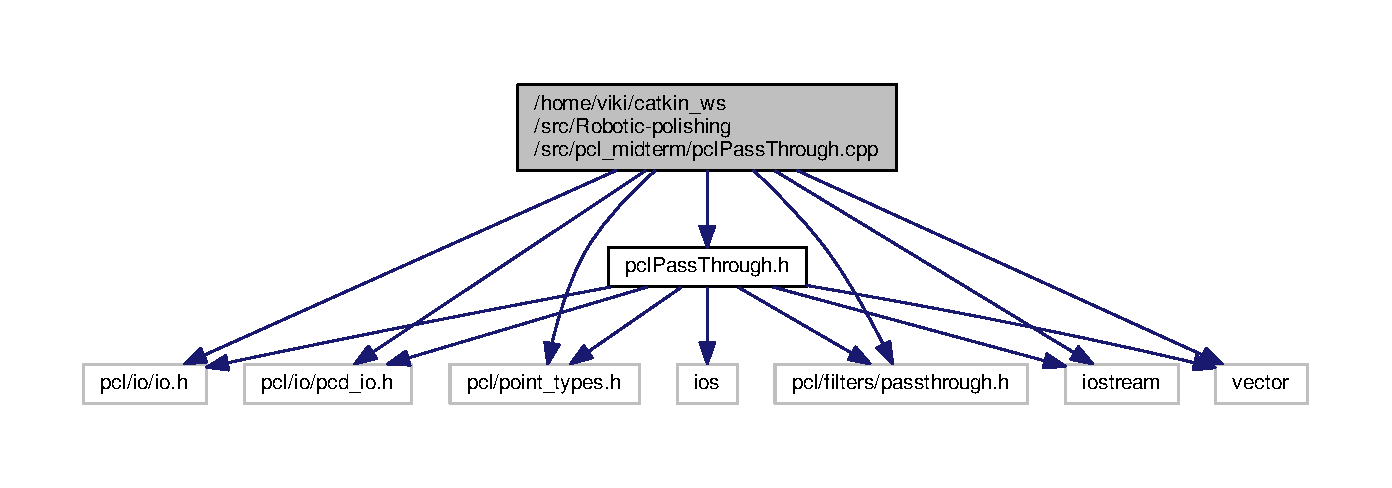
\includegraphics[width=350pt]{pclPassThrough_8cpp__incl}
\end{center}
\end{figure}


\subsection{Detailed Description}
This is the implementation of the \hyperlink{classpclPassThrough}{pcl\+Pass\+Through} class. This class consists of 7 methods. Please refer the \hyperlink{pclPassThrough_8h_source}{pcl\+Pass\+Through.\+h} for more detail. 

\begin{DoxyAuthor}{Author}
Michael Kam (michael081906) 
\end{DoxyAuthor}
\begin{DoxyRefDesc}{Bug}
\item[\hyperlink{bug__bug000034}{Bug}]No known bugs. \end{DoxyRefDesc}
\begin{DoxyCopyright}{Copyright}
G\+NU Public License.
\end{DoxyCopyright}
pcl\+Pass\+Throguh is free software\+: you can redistribute it and/or modify it under the terms of the G\+NU General Public License as published by the Free Software Foundation, either version 3 of the License, or (at your option) any later version.

pcl\+Pass\+Throguh is distributed in the hope that it will be useful, but W\+I\+T\+H\+O\+UT A\+NY W\+A\+R\+R\+A\+N\+TY; without even the implied warranty of M\+E\+R\+C\+H\+A\+N\+T\+A\+B\+I\+L\+I\+TY or F\+I\+T\+N\+E\+SS F\+OR A P\+A\+R\+T\+I\+C\+U\+L\+AR P\+U\+R\+P\+O\+SE. See the G\+NU General Public License for more details. You should have received a copy of the G\+NU General Public License along with pcl\+Pass\+Throguh. If not, see \href{http://www.gnu.org/licenses/}{\tt http\+://www.\+gnu.\+org/licenses/}. 
\hypertarget{pclStatisticalOutlierRemoval_8cpp}{}\section{/home/viki/catkin\+\_\+ws/src/\+Robotic-\/polishing/src/pcl\+\_\+midterm/pcl\+Statistical\+Outlier\+Removal.cpp File Reference}
\label{pclStatisticalOutlierRemoval_8cpp}\index{/home/viki/catkin\+\_\+ws/src/\+Robotic-\/polishing/src/pcl\+\_\+midterm/pcl\+Statistical\+Outlier\+Removal.\+cpp@{/home/viki/catkin\+\_\+ws/src/\+Robotic-\/polishing/src/pcl\+\_\+midterm/pcl\+Statistical\+Outlier\+Removal.\+cpp}}


This is the implementation of the pcl\+Statistical\+Outlier\+Removal class. This class consists of 7 methods. Please refer the \hyperlink{pclStatisticalOutlierRemoval_8h_source}{pcl\+Statistical\+Outlier\+Removal.\+h} for more detail.  


{\ttfamily \#include $<$pcl/io/io.\+h$>$}\\*
{\ttfamily \#include $<$pcl/io/pcd\+\_\+io.\+h$>$}\\*
{\ttfamily \#include $<$pcl/point\+\_\+types.\+h$>$}\\*
{\ttfamily \#include \char`\"{}pcl\+Statistical\+Outlier\+Removal.\+h\char`\"{}}\\*
{\ttfamily \#include $<$ios$>$}\\*
{\ttfamily \#include $<$iostream$>$}\\*
Include dependency graph for pcl\+Statistical\+Outlier\+Removal.\+cpp\+:
\nopagebreak
\begin{figure}[H]
\begin{center}
\leavevmode
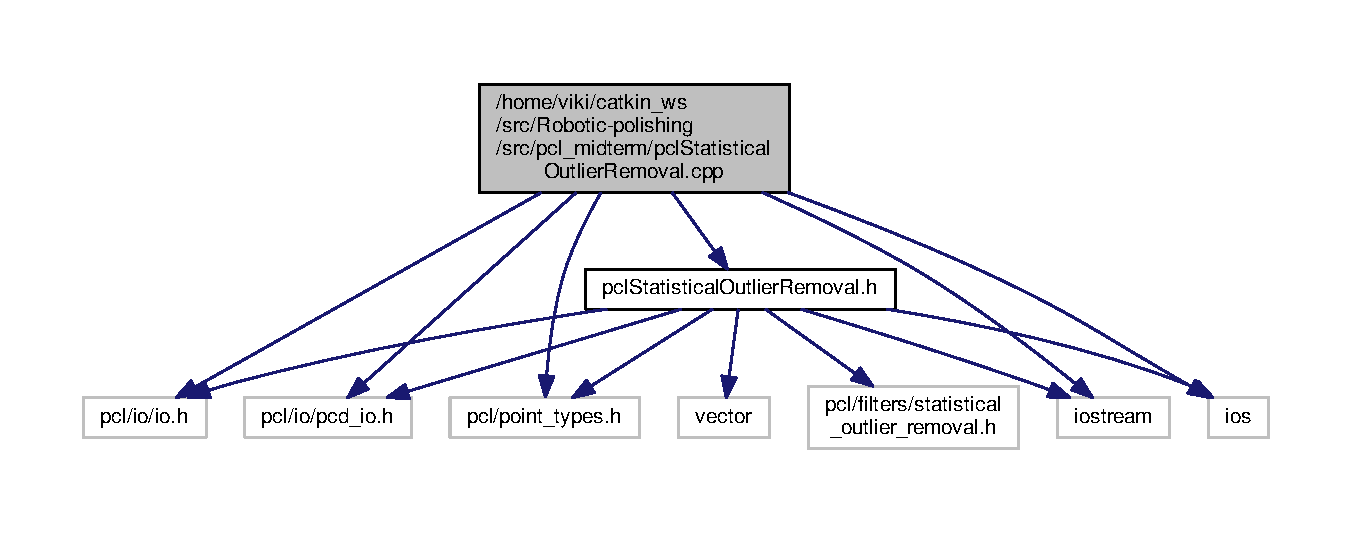
\includegraphics[width=350pt]{pclStatisticalOutlierRemoval_8cpp__incl}
\end{center}
\end{figure}


\subsection{Detailed Description}
This is the implementation of the pcl\+Statistical\+Outlier\+Removal class. This class consists of 7 methods. Please refer the \hyperlink{pclStatisticalOutlierRemoval_8h_source}{pcl\+Statistical\+Outlier\+Removal.\+h} for more detail. 

\begin{DoxyAuthor}{Author}
Michael Kam (michael081906) 
\end{DoxyAuthor}
\begin{DoxyRefDesc}{Bug}
\item[\hyperlink{bug__bug000035}{Bug}]No known bugs. \end{DoxyRefDesc}
\begin{DoxyCopyright}{Copyright}
G\+NU Public License.
\end{DoxyCopyright}
\hyperlink{classpclStatistOutRev}{pcl\+Statist\+Out\+Rev} is free software\+: you can redistribute it and/or modify it under the terms of the G\+NU General Public License as published by the Free Software Foundation, either version 3 of the License, or (at your option) any later version.

\hyperlink{classpclStatistOutRev}{pcl\+Statist\+Out\+Rev} is distributed in the hope that it will be useful, but W\+I\+T\+H\+O\+UT A\+NY W\+A\+R\+R\+A\+N\+TY; without even the implied warranty of M\+E\+R\+C\+H\+A\+N\+T\+A\+B\+I\+L\+I\+TY or F\+I\+T\+N\+E\+SS F\+OR A P\+A\+R\+T\+I\+C\+U\+L\+AR P\+U\+R\+P\+O\+SE. See the G\+NU General Public License for more details. You should have received a copy of the G\+NU General Public License along with \hyperlink{classpclStatistOutRev}{pcl\+Statist\+Out\+Rev}. If not, see \href{http://www.gnu.org/licenses/}{\tt http\+://www.\+gnu.\+org/licenses/}. 
\hypertarget{pclVoxel_8cpp}{}\section{/home/viki/catkin\+\_\+ws/src/\+Robotic-\/polishing/src/pcl\+\_\+midterm/pcl\+Voxel.cpp File Reference}
\label{pclVoxel_8cpp}\index{/home/viki/catkin\+\_\+ws/src/\+Robotic-\/polishing/src/pcl\+\_\+midterm/pcl\+Voxel.\+cpp@{/home/viki/catkin\+\_\+ws/src/\+Robotic-\/polishing/src/pcl\+\_\+midterm/pcl\+Voxel.\+cpp}}


This is the implementation of the \hyperlink{classpclVoxel}{pcl\+Voxel} class. This class consists of 5 methods. Please refer the \hyperlink{pclVoxel_8h}{pcl\+Voxel.\+h} for more detail.  


{\ttfamily \#include $<$pcl/io/pcd\+\_\+io.\+h$>$}\\*
{\ttfamily \#include $<$pcl/point\+\_\+types.\+h$>$}\\*
{\ttfamily \#include $<$pcl/filters/voxel\+\_\+grid.\+h$>$}\\*
{\ttfamily \#include \char`\"{}pcl\+Voxel.\+h\char`\"{}}\\*
{\ttfamily \#include $<$iostream$>$}\\*
{\ttfamily \#include $<$vector$>$}\\*
{\ttfamily \#include $<$ios$>$}\\*
Include dependency graph for pcl\+Voxel.\+cpp\+:
\nopagebreak
\begin{figure}[H]
\begin{center}
\leavevmode
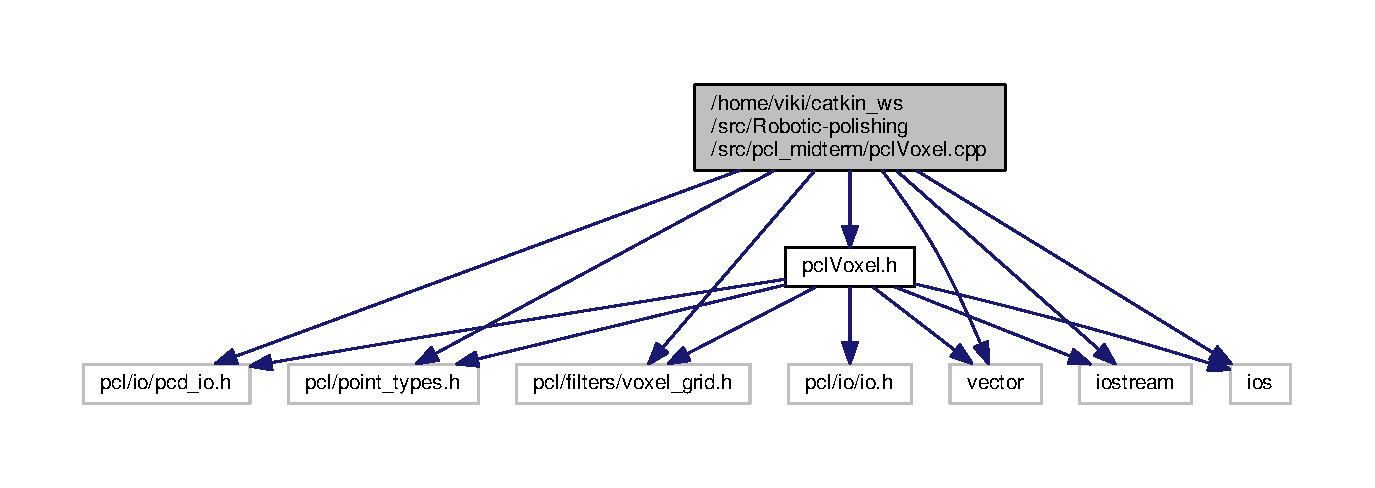
\includegraphics[width=350pt]{pclVoxel_8cpp__incl}
\end{center}
\end{figure}


\subsection{Detailed Description}
This is the implementation of the \hyperlink{classpclVoxel}{pcl\+Voxel} class. This class consists of 5 methods. Please refer the \hyperlink{pclVoxel_8h}{pcl\+Voxel.\+h} for more detail. 

\begin{DoxyAuthor}{Author}
Michael Kam (michael081906) 
\end{DoxyAuthor}
\begin{DoxyRefDesc}{Bug}
\item[\hyperlink{bug__bug000036}{Bug}]No known bugs. \end{DoxyRefDesc}
\begin{DoxyCopyright}{Copyright}
G\+NU Public License.
\end{DoxyCopyright}
\hyperlink{classpclVoxel}{pcl\+Voxel} is free software\+: you can redistribute it and/or modify it under the terms of the G\+NU General Public License as published by the Free Software Foundation, either version 3 of the License, or (at your option) any later version.

\hyperlink{classpclVoxel}{pcl\+Voxel} is distributed in the hope that it will be useful, but W\+I\+T\+H\+O\+UT A\+NY W\+A\+R\+R\+A\+N\+TY; without even the implied warranty of M\+E\+R\+C\+H\+A\+N\+T\+A\+B\+I\+L\+I\+TY or F\+I\+T\+N\+E\+SS F\+OR A P\+A\+R\+T\+I\+C\+U\+L\+AR P\+U\+R\+P\+O\+SE. See the G\+NU General Public License for more details. You should have received a copy of the G\+NU General Public License along with \hyperlink{classpclVoxel}{pcl\+Voxel}. If not, see \href{http://www.gnu.org/licenses/}{\tt http\+://www.\+gnu.\+org/licenses/}. 
\hypertarget{talker_8cpp}{}\section{/home/viki/catkin\+\_\+ws/src/\+Robotic-\/polishing/src/talker.cpp File Reference}
\label{talker_8cpp}\index{/home/viki/catkin\+\_\+ws/src/\+Robotic-\/polishing/src/talker.\+cpp@{/home/viki/catkin\+\_\+ws/src/\+Robotic-\/polishing/src/talker.\+cpp}}


This \hyperlink{talker_8cpp}{talker.\+cpp} is a ros node that subscribes point cloud and computes the trajectory f.  


{\ttfamily \#include \char`\"{}ros/ros.\+h\char`\"{}}\\*
{\ttfamily \#include \char`\"{}std\+\_\+msgs/\+String.\+h\char`\"{}}\\*
{\ttfamily \#include \char`\"{}s\+\_\+hull\+\_\+pro.\+h\char`\"{}}\\*
{\ttfamily \#include \char`\"{}pcl\+Io.\+h\char`\"{}}\\*
{\ttfamily \#include \char`\"{}pcl\+Voxel.\+h\char`\"{}}\\*
{\ttfamily \#include \char`\"{}pcl\+Mls\+Smoothing.\+h\char`\"{}}\\*
{\ttfamily \#include \char`\"{}pcl\+Pass\+Through.\+h\char`\"{}}\\*
{\ttfamily \#include \char`\"{}pcl\+Statistical\+Outlier\+Removal.\+h\char`\"{}}\\*
{\ttfamily \#include \char`\"{}pcl\+Fast\+Triangular.\+h\char`\"{}}\\*
{\ttfamily \#include \char`\"{}pcl\+Cloud\+Viewer.\+h\char`\"{}}\\*
{\ttfamily \#include \char`\"{}find\+Nearest\+Point.\+h\char`\"{}}\\*
{\ttfamily \#include \char`\"{}delaunay3.\+h\char`\"{}}\\*
{\ttfamily \#include \char`\"{}dijkstra\+P\+Q.\+h\char`\"{}}\\*
{\ttfamily \#include $<$pcl/io/io.\+h$>$}\\*
{\ttfamily \#include $<$pcl/io/pcd\+\_\+io.\+h$>$}\\*
{\ttfamily \#include $<$pcl/point\+\_\+types.\+h$>$}\\*
{\ttfamily \#include $<$pcl/filters/statistical\+\_\+outlier\+\_\+removal.\+h$>$}\\*
{\ttfamily \#include $<$pcl/visualization/cloud\+\_\+viewer.\+h$>$}\\*
{\ttfamily \#include $<$pcl/filters/radius\+\_\+outlier\+\_\+removal.\+h$>$}\\*
{\ttfamily \#include $<$pcl/filters/conditional\+\_\+removal.\+h$>$}\\*
{\ttfamily \#include $<$iostream$>$}\\*
{\ttfamily \#include $<$queue$>$}\\*
{\ttfamily \#include $<$stack$>$}\\*
{\ttfamily \#include $<$limits$>$}\\*
{\ttfamily \#include $<$algorithm$>$}\\*
{\ttfamily \#include $<$stdio.\+h$>$}\\*
{\ttfamily \#include $<$stdlib.\+h$>$}\\*
{\ttfamily \#include $<$hash\+\_\+set$>$}\\*
{\ttfamily \#include $<$ctype.\+h$>$}\\*
{\ttfamily \#include $<$string.\+h$>$}\\*
{\ttfamily \#include $<$string$>$}\\*
{\ttfamily \#include $<$sys/types.\+h$>$}\\*
{\ttfamily \#include $<$set$>$}\\*
{\ttfamily \#include $<$vector$>$}\\*
{\ttfamily \#include $<$fstream$>$}\\*
{\ttfamily \#include $<$math.\+h$>$}\\*
{\ttfamily \#include $<$time.\+h$>$}\\*
{\ttfamily \#include $<$sstream$>$}\\*
{\ttfamily \#include $<$pcl\+\_\+ros/point\+\_\+cloud.\+h$>$}\\*
{\ttfamily \#include $<$sensor\+\_\+msgs/\+Point\+Cloud2.\+h$>$}\\*
{\ttfamily \#include \char`\"{}robotic\+\_\+polishing/\+Trajectory.\+h\char`\"{}}\\*
{\ttfamily \#include $<$pcl\+\_\+conversions/pcl\+\_\+conversions.\+h$>$}\\*
{\ttfamily \#include $<$pcl\+\_\+ros/transforms.\+h$>$}\\*
Include dependency graph for talker.\+cpp\+:
\nopagebreak
\begin{figure}[H]
\begin{center}
\leavevmode
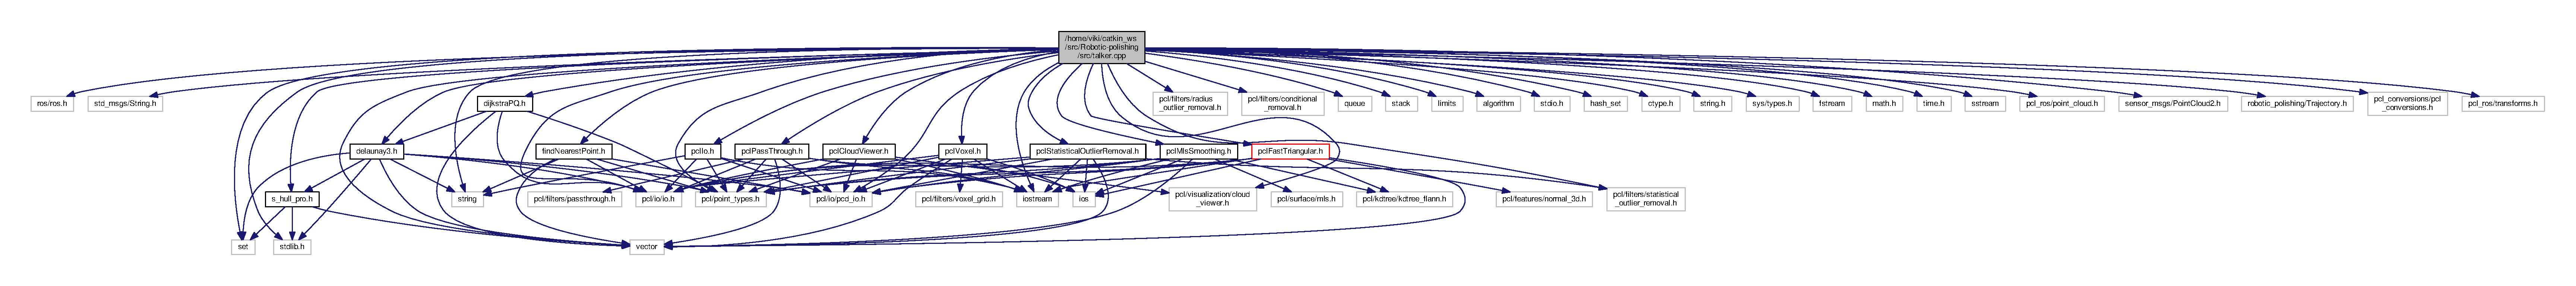
\includegraphics[width=350pt]{talker_8cpp__incl}
\end{center}
\end{figure}
\subsection*{Typedefs}
\begin{DoxyCompactItemize}
\item 
typedef pcl\+::\+Point\+Cloud$<$ pcl\+::\+Point\+X\+YZ $>$ {\bfseries Point\+Cloud}\hypertarget{talker_8cpp_a6c737bbce051bc4690e4c608adc2deec}{}\label{talker_8cpp_a6c737bbce051bc4690e4c608adc2deec}

\end{DoxyCompactItemize}
\subsection*{Functions}
\begin{DoxyCompactItemize}
\item 
void \hyperlink{talker_8cpp_a284e0e47d3aae6d849b820ab8985a966}{callback} (const sensor\+\_\+msgs\+::\+Point\+Cloud2\+Ptr \&cloud)
\begin{DoxyCompactList}\small\item\em callback is a callback function that subscribes the point cloud data and uses tf to transform to world coordinate \end{DoxyCompactList}\item 
bool \hyperlink{talker_8cpp_a0a850b1779efa9cd37089e6f5a2c3200}{find} (robotic\+\_\+polishing\+::\+Trajectory\+::\+Request \&req, robotic\+\_\+polishing\+::\+Trajectory\+::\+Response \&res)
\begin{DoxyCompactList}\small\item\em get\+\_\+joints is a callback function that subscribe the joint position data and set it into joints vector \end{DoxyCompactList}\item 
int \hyperlink{talker_8cpp_a3c04138a5bfe5d72780bb7e82a18e627}{main} (int argc, char $\ast$$\ast$argv)
\end{DoxyCompactItemize}
\subsection*{Variables}
\begin{DoxyCompactItemize}
\item 
Point\+Cloud {\bfseries pointcloud\+\_\+in}\hypertarget{talker_8cpp_aaf642a9de8c488cf8e26f3d008494f94}{}\label{talker_8cpp_aaf642a9de8c488cf8e26f3d008494f94}

\item 
Point\+Cloud {\bfseries pointcloud\+\_\+out}\hypertarget{talker_8cpp_a09a14efc015b6ec457716cc95a141156}{}\label{talker_8cpp_a09a14efc015b6ec457716cc95a141156}

\end{DoxyCompactItemize}


\subsection{Detailed Description}
This \hyperlink{talker_8cpp}{talker.\+cpp} is a ros node that subscribes point cloud and computes the trajectory f. 

\begin{DoxyAuthor}{Author}
Michael Kam (michael081906) 
\end{DoxyAuthor}
\begin{DoxyRefDesc}{Bug}
\item[\hyperlink{bug__bug000024}{Bug}]No known bugs. \end{DoxyRefDesc}
\begin{DoxyCopyright}{Copyright}
G\+NU Public License.
\end{DoxyCopyright}
talker is free software\+: you can redistribute it and/or modify it under the terms of the G\+NU General Public License as published by the Free Software Foundation, either version 3 of the License, or (at your option) any later version.

talker is distributed in the hope that it will be useful, but W\+I\+T\+H\+O\+UT A\+NY W\+A\+R\+R\+A\+N\+TY; without even the implied warranty of M\+E\+R\+C\+H\+A\+N\+T\+A\+B\+I\+L\+I\+TY or F\+I\+T\+N\+E\+SS F\+OR A P\+A\+R\+T\+I\+C\+U\+L\+AR P\+U\+R\+P\+O\+SE. See the G\+NU General Public License for more details. You should have received a copy of the G\+NU General Public License along with talker. If not, see \href{http://www.gnu.org/licenses/}{\tt http\+://www.\+gnu.\+org/licenses/}. 

\subsection{Function Documentation}
\index{talker.\+cpp@{talker.\+cpp}!callback@{callback}}
\index{callback@{callback}!talker.\+cpp@{talker.\+cpp}}
\subsubsection[{\texorpdfstring{callback(const sensor\+\_\+msgs\+::\+Point\+Cloud2\+Ptr \&cloud)}{callback(const sensor_msgs::PointCloud2Ptr &cloud)}}]{\setlength{\rightskip}{0pt plus 5cm}void callback (
\begin{DoxyParamCaption}
\item[{const sensor\+\_\+msgs\+::\+Point\+Cloud2\+Ptr \&}]{cloud}
\end{DoxyParamCaption}
)}\hypertarget{talker_8cpp_a284e0e47d3aae6d849b820ab8985a966}{}\label{talker_8cpp_a284e0e47d3aae6d849b820ab8985a966}


callback is a callback function that subscribes the point cloud data and uses tf to transform to world coordinate 


\begin{DoxyParams}[1]{Parameters}
\mbox{\tt in}  & {\em cloud} & sensor\+\_\+msgs\+::\+Point\+Cloud2\+Ptr that contains point cloud information \\
\hline
\end{DoxyParams}
\begin{DoxyReturn}{Returns}
none 
\end{DoxyReturn}
\index{talker.\+cpp@{talker.\+cpp}!find@{find}}
\index{find@{find}!talker.\+cpp@{talker.\+cpp}}
\subsubsection[{\texorpdfstring{find(robotic\+\_\+polishing\+::\+Trajectory\+::\+Request \&req, robotic\+\_\+polishing\+::\+Trajectory\+::\+Response \&res)}{find(robotic_polishing::Trajectory::Request &req, robotic_polishing::Trajectory::Response &res)}}]{\setlength{\rightskip}{0pt plus 5cm}bool find (
\begin{DoxyParamCaption}
\item[{robotic\+\_\+polishing\+::\+Trajectory\+::\+Request \&}]{req, }
\item[{robotic\+\_\+polishing\+::\+Trajectory\+::\+Response \&}]{res}
\end{DoxyParamCaption}
)}\hypertarget{talker_8cpp_a0a850b1779efa9cd37089e6f5a2c3200}{}\label{talker_8cpp_a0a850b1779efa9cd37089e6f5a2c3200}


get\+\_\+joints is a callback function that subscribe the joint position data and set it into joints vector 


\begin{DoxyParams}[1]{Parameters}
\mbox{\tt in}  & {\em data} & sensor\+\_\+msgs\+::\+Joint\+State that contains joint position \\
\hline
\end{DoxyParams}
\begin{DoxyReturn}{Returns}
nonefind is a service for computing trajectory based on a start and an end point. 
\end{DoxyReturn}

\begin{DoxyParams}[1]{Parameters}
\mbox{\tt in}  & {\em req} & is a request that contains coordinates of start and end point. \\
\hline
\mbox{\tt in}  & {\em res} & is a response that contains trajectory information \\
\hline
\end{DoxyParams}
\begin{DoxyReturn}{Returns}
none 
\end{DoxyReturn}
\index{talker.\+cpp@{talker.\+cpp}!main@{main}}
\index{main@{main}!talker.\+cpp@{talker.\+cpp}}
\subsubsection[{\texorpdfstring{main(int argc, char $\ast$$\ast$argv)}{main(int argc, char **argv)}}]{\setlength{\rightskip}{0pt plus 5cm}int main (
\begin{DoxyParamCaption}
\item[{int}]{argc, }
\item[{char $\ast$$\ast$}]{argv}
\end{DoxyParamCaption}
)}\hypertarget{talker_8cpp_a3c04138a5bfe5d72780bb7e82a18e627}{}\label{talker_8cpp_a3c04138a5bfe5d72780bb7e82a18e627}
This tutorial demonstrates simple sending of messages over the R\+OS system. 
\hypertarget{main_8cpp}{}\section{/home/viki/catkin\+\_\+ws/src/\+Robotic-\/polishing/test/main.cpp File Reference}
\label{main_8cpp}\index{/home/viki/catkin\+\_\+ws/src/\+Robotic-\/polishing/test/main.\+cpp@{/home/viki/catkin\+\_\+ws/src/\+Robotic-\/polishing/test/main.\+cpp}}


main test file of this project.  


{\ttfamily \#include $<$gtest/gtest.\+h$>$}\\*
{\ttfamily \#include $<$ros/console.\+h$>$}\\*
{\ttfamily \#include \char`\"{}ros/ros.\+h\char`\"{}}\\*
Include dependency graph for main.\+cpp\+:
\nopagebreak
\begin{figure}[H]
\begin{center}
\leavevmode
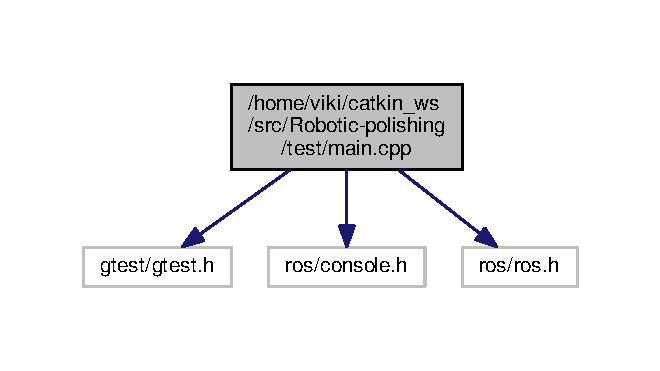
\includegraphics[width=317pt]{main_8cpp__incl}
\end{center}
\end{figure}
\subsection*{Functions}
\begin{DoxyCompactItemize}
\item 
int {\bfseries main} (int argc, char $\ast$$\ast$argv)\hypertarget{main_8cpp_a3c04138a5bfe5d72780bb7e82a18e627}{}\label{main_8cpp_a3c04138a5bfe5d72780bb7e82a18e627}

\end{DoxyCompactItemize}


\subsection{Detailed Description}
main test file of this project. 

The cpp-\/test start entering this file.

\begin{DoxyAuthor}{Author}
Michael Kam (michael081906) 
\end{DoxyAuthor}
\begin{DoxyRefDesc}{Bug}
\item[\hyperlink{bug__bug000037}{Bug}]No known bugs. \end{DoxyRefDesc}
\begin{DoxyCopyright}{Copyright}
G\+NU Public License. 
\end{DoxyCopyright}

\hypertarget{pclFastTriangularTest_8cpp}{}\section{/home/viki/catkin\+\_\+ws/src/\+Robotic-\/polishing/test/pcl\+Fast\+Triangular\+Test.cpp File Reference}
\label{pclFastTriangularTest_8cpp}\index{/home/viki/catkin\+\_\+ws/src/\+Robotic-\/polishing/test/pcl\+Fast\+Triangular\+Test.\+cpp@{/home/viki/catkin\+\_\+ws/src/\+Robotic-\/polishing/test/pcl\+Fast\+Triangular\+Test.\+cpp}}


\hyperlink{pclFastTriangularTest_8cpp}{pcl\+Fast\+Triangular\+Test.\+cpp} consists of 3 unit test cases that test the \hyperlink{classpclFastTriangular}{pcl\+Fast\+Triangular} class.  


{\ttfamily \#include $<$gtest/gtest.\+h$>$}\\*
{\ttfamily \#include $<$pcl\+Fast\+Triangular.\+h$>$}\\*
{\ttfamily \#include $<$pcl\+Mls\+Smoothing.\+h$>$}\\*
{\ttfamily \#include $<$vector$>$}\\*
Include dependency graph for pcl\+Fast\+Triangular\+Test.\+cpp\+:
\nopagebreak
\begin{figure}[H]
\begin{center}
\leavevmode
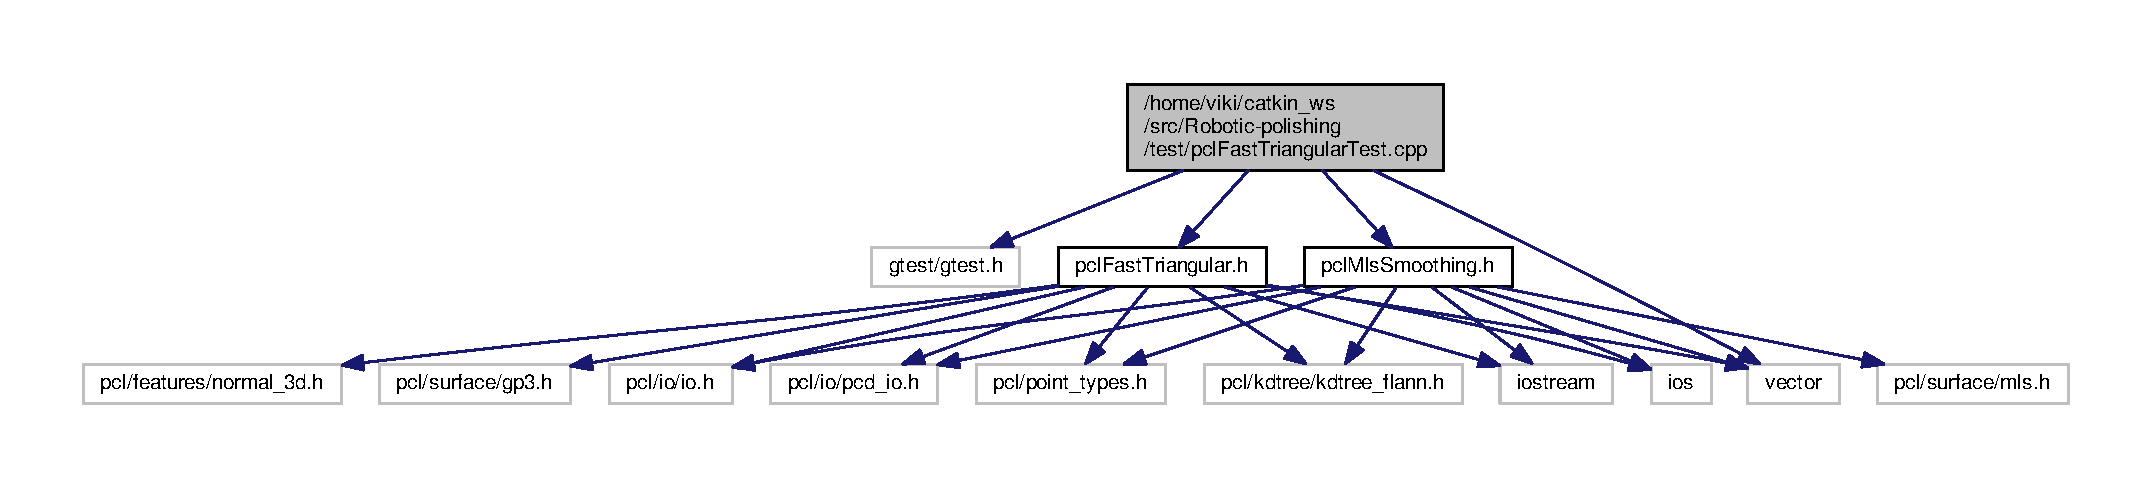
\includegraphics[width=350pt]{pclFastTriangularTest_8cpp__incl}
\end{center}
\end{figure}
\subsection*{Functions}
\begin{DoxyCompactItemize}
\item 
\hyperlink{pclFastTriangularTest_8cpp_a8c383ad3501d8f92cc08103bc7a6f1f5}{T\+E\+ST} (pcl\+Fast\+Triangular\+Test, set\+Radius)\hypertarget{pclFastTriangularTest_8cpp_a8c383ad3501d8f92cc08103bc7a6f1f5}{}\label{pclFastTriangularTest_8cpp_a8c383ad3501d8f92cc08103bc7a6f1f5}

\begin{DoxyCompactList}\small\item\em \hyperlink{pclFastTriangularTest_8cpp_a8c383ad3501d8f92cc08103bc7a6f1f5}{T\+E\+S\+T(pcl\+Fast\+Triangular\+Test, set\+Radius)} will test the set\+Search\+Radius() and get\+Search\+Radius() method. \end{DoxyCompactList}\item 
\hyperlink{pclFastTriangularTest_8cpp_af434c6da69e2cf5de786e4304039d16a}{T\+E\+ST} (pcl\+Fast\+Triangular\+Test, setpcl\+Cloud)\hypertarget{pclFastTriangularTest_8cpp_af434c6da69e2cf5de786e4304039d16a}{}\label{pclFastTriangularTest_8cpp_af434c6da69e2cf5de786e4304039d16a}

\begin{DoxyCompactList}\small\item\em \hyperlink{pclFastTriangularTest_8cpp_af434c6da69e2cf5de786e4304039d16a}{T\+E\+S\+T(pcl\+Fast\+Triangular\+Test, setpcl\+Cloud)} will test the set\+Input\+Cloud() and get\+Input\+Cloud() method. \end{DoxyCompactList}\item 
\hyperlink{pclFastTriangularTest_8cpp_a72dc83c0acb55b59e3dd8bff64ebf8b3}{T\+E\+ST} (pcl\+Fast\+Triangular\+Test, Triangular\+Mesh)\hypertarget{pclFastTriangularTest_8cpp_a72dc83c0acb55b59e3dd8bff64ebf8b3}{}\label{pclFastTriangularTest_8cpp_a72dc83c0acb55b59e3dd8bff64ebf8b3}

\begin{DoxyCompactList}\small\item\em \hyperlink{pclFastTriangularTest_8cpp_a72dc83c0acb55b59e3dd8bff64ebf8b3}{T\+E\+S\+T(pcl\+Fast\+Triangular\+Test, Triangular\+Mesh)} will test the reconctruct() method. \end{DoxyCompactList}\end{DoxyCompactItemize}


\subsection{Detailed Description}
\hyperlink{pclFastTriangularTest_8cpp}{pcl\+Fast\+Triangular\+Test.\+cpp} consists of 3 unit test cases that test the \hyperlink{classpclFastTriangular}{pcl\+Fast\+Triangular} class. 

\hyperlink{pclFastTriangularTest_8cpp_a8c383ad3501d8f92cc08103bc7a6f1f5}{T\+E\+S\+T(pcl\+Fast\+Triangular\+Test, set\+Radius)} will test the set\+Search\+Radius() and get\+Search\+Radius() method. \hyperlink{pclFastTriangularTest_8cpp_af434c6da69e2cf5de786e4304039d16a}{T\+E\+S\+T(pcl\+Fast\+Triangular\+Test, setpcl\+Cloud)} will test the set\+Input\+Cloud() and get\+Input\+Cloud() method. \hyperlink{pclFastTriangularTest_8cpp_a72dc83c0acb55b59e3dd8bff64ebf8b3}{T\+E\+S\+T(pcl\+Fast\+Triangular\+Test, Triangular\+Mesh)} will test the reconctruct() method.

\begin{DoxyAuthor}{Author}
Michael Kam (michael081906) 
\end{DoxyAuthor}
\begin{DoxyRefDesc}{Bug}
\item[\hyperlink{bug__bug000038}{Bug}]No known bugs. \end{DoxyRefDesc}
\begin{DoxyCopyright}{Copyright}
G\+NU Public License. 
\end{DoxyCopyright}

\hypertarget{pclIoTest_8cpp}{}\section{/home/viki/catkin\+\_\+ws/src/\+Robotic-\/polishing/test/pcl\+Io\+Test.cpp File Reference}
\label{pclIoTest_8cpp}\index{/home/viki/catkin\+\_\+ws/src/\+Robotic-\/polishing/test/pcl\+Io\+Test.\+cpp@{/home/viki/catkin\+\_\+ws/src/\+Robotic-\/polishing/test/pcl\+Io\+Test.\+cpp}}


\hyperlink{pclIoTest_8cpp}{pcl\+Io\+Test.\+cpp} consists of 2 unit test cases that test the \hyperlink{classpclIo}{pcl\+Io} class.  


{\ttfamily \#include \char`\"{}pcl\+Io.\+h\char`\"{}}\\*
{\ttfamily \#include $<$pcl/io/pcd\+\_\+io.\+h$>$}\\*
{\ttfamily \#include $<$pcl/point\+\_\+types.\+h$>$}\\*
{\ttfamily \#include $<$gtest/gtest.\+h$>$}\\*
{\ttfamily \#include $<$iostream$>$}\\*
Include dependency graph for pcl\+Io\+Test.\+cpp\+:
\nopagebreak
\begin{figure}[H]
\begin{center}
\leavevmode
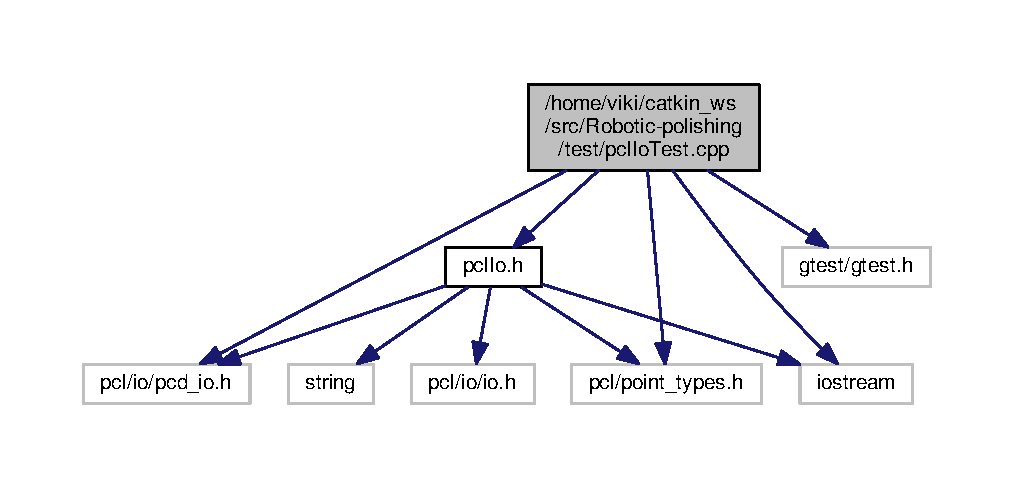
\includegraphics[width=350pt]{pclIoTest_8cpp__incl}
\end{center}
\end{figure}
\subsection*{Functions}
\begin{DoxyCompactItemize}
\item 
\hyperlink{pclIoTest_8cpp_acadc143b86b8db1747d4dfd44ae475e3}{T\+E\+ST} (pcl\+Io\+Test, load\+P\+C\+Dfile\+Must\+Fail)\hypertarget{pclIoTest_8cpp_acadc143b86b8db1747d4dfd44ae475e3}{}\label{pclIoTest_8cpp_acadc143b86b8db1747d4dfd44ae475e3}

\begin{DoxyCompactList}\small\item\em \hyperlink{pclIoTest_8cpp_acadc143b86b8db1747d4dfd44ae475e3}{T\+E\+S\+T(pcl\+Io\+Test, load\+P\+C\+Dfile\+Must\+Fail)} will test the read\+P\+C\+Dfile() method. \end{DoxyCompactList}\item 
\hyperlink{pclIoTest_8cpp_aaf03e3af6aa987fa78da874364eaf931}{T\+E\+ST} (pcl\+Io\+Test, load\+P\+C\+Dfile\+Show\+Result)\hypertarget{pclIoTest_8cpp_aaf03e3af6aa987fa78da874364eaf931}{}\label{pclIoTest_8cpp_aaf03e3af6aa987fa78da874364eaf931}

\begin{DoxyCompactList}\small\item\em \hyperlink{pclIoTest_8cpp_aaf03e3af6aa987fa78da874364eaf931}{T\+E\+S\+T(pcl\+Io\+Test, load\+P\+C\+Dfile\+Show\+Result)} will test the get\+Point\+Cloud() method. \end{DoxyCompactList}\end{DoxyCompactItemize}


\subsection{Detailed Description}
\hyperlink{pclIoTest_8cpp}{pcl\+Io\+Test.\+cpp} consists of 2 unit test cases that test the \hyperlink{classpclIo}{pcl\+Io} class. 

\hyperlink{pclIoTest_8cpp_acadc143b86b8db1747d4dfd44ae475e3}{T\+E\+S\+T(pcl\+Io\+Test, load\+P\+C\+Dfile\+Must\+Fail)} will test the read\+P\+C\+Dfile() method. \hyperlink{pclIoTest_8cpp_aaf03e3af6aa987fa78da874364eaf931}{T\+E\+S\+T(pcl\+Io\+Test, load\+P\+C\+Dfile\+Show\+Result)} will test the get\+Point\+Cloud() method.

\begin{DoxyAuthor}{Author}
Michael Kam (michael081906) 
\end{DoxyAuthor}
\begin{DoxyRefDesc}{Bug}
\item[\hyperlink{bug__bug000039}{Bug}]No known bugs. \end{DoxyRefDesc}
\begin{DoxyCopyright}{Copyright}
G\+NU Public License. 
\end{DoxyCopyright}

\hypertarget{pclMlsSmoothingTest_8cpp}{}\section{/home/viki/catkin\+\_\+ws/src/\+Robotic-\/polishing/test/pcl\+Mls\+Smoothing\+Test.cpp File Reference}
\label{pclMlsSmoothingTest_8cpp}\index{/home/viki/catkin\+\_\+ws/src/\+Robotic-\/polishing/test/pcl\+Mls\+Smoothing\+Test.\+cpp@{/home/viki/catkin\+\_\+ws/src/\+Robotic-\/polishing/test/pcl\+Mls\+Smoothing\+Test.\+cpp}}


\hyperlink{pclMlsSmoothingTest_8cpp}{pcl\+Mls\+Smoothing\+Test.\+cpp} consists of 3 unit test cases that test the \hyperlink{classpclMlsSmoothing}{pcl\+Mls\+Smoothing} class.  


{\ttfamily \#include $<$gtest/gtest.\+h$>$}\\*
{\ttfamily \#include $<$pcl\+Mls\+Smoothing.\+h$>$}\\*
Include dependency graph for pcl\+Mls\+Smoothing\+Test.\+cpp\+:
\nopagebreak
\begin{figure}[H]
\begin{center}
\leavevmode
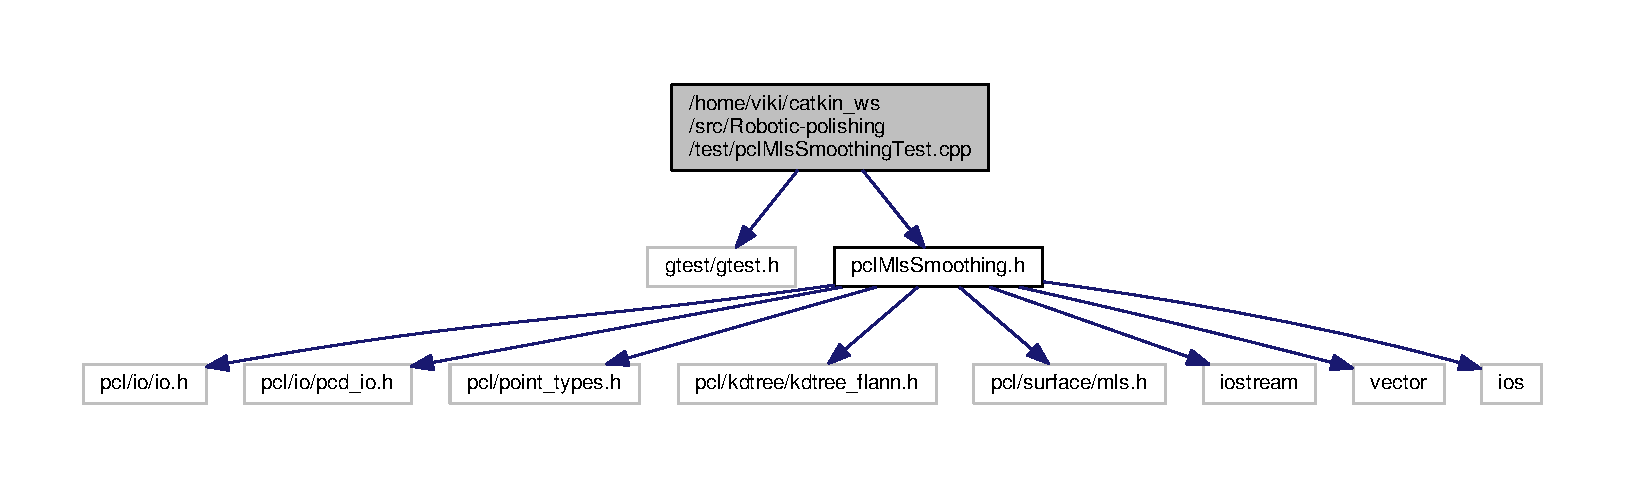
\includegraphics[width=350pt]{pclMlsSmoothingTest_8cpp__incl}
\end{center}
\end{figure}
\subsection*{Functions}
\begin{DoxyCompactItemize}
\item 
\hyperlink{pclMlsSmoothingTest_8cpp_a108228ab9f6b7dc193551c5025b26b69}{T\+E\+ST} (pcl\+Mls\+Smoothing\+Test, set\+Radius)\hypertarget{pclMlsSmoothingTest_8cpp_a108228ab9f6b7dc193551c5025b26b69}{}\label{pclMlsSmoothingTest_8cpp_a108228ab9f6b7dc193551c5025b26b69}

\begin{DoxyCompactList}\small\item\em \hyperlink{pclMlsSmoothingTest_8cpp_a108228ab9f6b7dc193551c5025b26b69}{T\+E\+S\+T(pcl\+Mls\+Smoothing\+Test, set\+Radius)} will test the set\+Search\+Radius() and get\+Search\+Radius() method. \end{DoxyCompactList}\item 
\hyperlink{pclMlsSmoothingTest_8cpp_a0f0895afe16f423a9b57b8da0f4a2749}{T\+E\+ST} (pcl\+Mls\+Smoothing\+Test, setpcl\+Cloud)\hypertarget{pclMlsSmoothingTest_8cpp_a0f0895afe16f423a9b57b8da0f4a2749}{}\label{pclMlsSmoothingTest_8cpp_a0f0895afe16f423a9b57b8da0f4a2749}

\begin{DoxyCompactList}\small\item\em \hyperlink{pclMlsSmoothingTest_8cpp_a0f0895afe16f423a9b57b8da0f4a2749}{T\+E\+S\+T(pcl\+Mls\+Smoothing\+Test, setpcl\+Cloud)} will test the get\+Input\+Cloud() and set\+Input\+Cloud() method. \end{DoxyCompactList}\item 
\hyperlink{pclMlsSmoothingTest_8cpp_a2438d2c1b948a4136db5fcb288f9ca87}{T\+E\+ST} (pcl\+Mls\+Smoothing\+Test, Mls\+Filtering)\hypertarget{pclMlsSmoothingTest_8cpp_a2438d2c1b948a4136db5fcb288f9ca87}{}\label{pclMlsSmoothingTest_8cpp_a2438d2c1b948a4136db5fcb288f9ca87}

\begin{DoxyCompactList}\small\item\em \hyperlink{pclMlsSmoothingTest_8cpp_a2438d2c1b948a4136db5fcb288f9ca87}{T\+E\+S\+T(pcl\+Mls\+Smoothing\+Test, Mls\+Filtering)} will test the mls\+Process() \end{DoxyCompactList}\end{DoxyCompactItemize}


\subsection{Detailed Description}
\hyperlink{pclMlsSmoothingTest_8cpp}{pcl\+Mls\+Smoothing\+Test.\+cpp} consists of 3 unit test cases that test the \hyperlink{classpclMlsSmoothing}{pcl\+Mls\+Smoothing} class. 

\hyperlink{pclMlsSmoothingTest_8cpp_a108228ab9f6b7dc193551c5025b26b69}{T\+E\+S\+T(pcl\+Mls\+Smoothing\+Test, set\+Radius)} will test the set\+Search\+Radius() and get\+Search\+Radius() method. \hyperlink{pclMlsSmoothingTest_8cpp_a0f0895afe16f423a9b57b8da0f4a2749}{T\+E\+S\+T(pcl\+Mls\+Smoothing\+Test, setpcl\+Cloud)} will test the get\+Input\+Cloud() and set\+Input\+Cloud() method. \hyperlink{pclMlsSmoothingTest_8cpp_a2438d2c1b948a4136db5fcb288f9ca87}{T\+E\+S\+T(pcl\+Mls\+Smoothing\+Test, Mls\+Filtering)} will test the mls\+Process().

\begin{DoxyAuthor}{Author}
Michael Kam (michael081906) 
\end{DoxyAuthor}
\begin{DoxyRefDesc}{Bug}
\item[\hyperlink{bug__bug000040}{Bug}]No known bugs. \end{DoxyRefDesc}
\begin{DoxyCopyright}{Copyright}
G\+NU Public License. 
\end{DoxyCopyright}

\hypertarget{pclPassThroughTest_8cpp}{}\section{/home/viki/catkin\+\_\+ws/src/\+Robotic-\/polishing/test/pcl\+Pass\+Through\+Test.cpp File Reference}
\label{pclPassThroughTest_8cpp}\index{/home/viki/catkin\+\_\+ws/src/\+Robotic-\/polishing/test/pcl\+Pass\+Through\+Test.\+cpp@{/home/viki/catkin\+\_\+ws/src/\+Robotic-\/polishing/test/pcl\+Pass\+Through\+Test.\+cpp}}


\hyperlink{pclPassThroughTest_8cpp}{pcl\+Pass\+Through\+Test.\+cpp} consists of 2 unit test cases that test the \hyperlink{classpclPassThrough}{pcl\+Pass\+Through} class.  


{\ttfamily \#include \char`\"{}pcl\+Io.\+h\char`\"{}}\\*
{\ttfamily \#include \char`\"{}pcl\+Pass\+Through.\+h\char`\"{}}\\*
{\ttfamily \#include $<$gtest/gtest.\+h$>$}\\*
{\ttfamily \#include $<$pcl/io/pcd\+\_\+io.\+h$>$}\\*
{\ttfamily \#include $<$pcl/point\+\_\+types.\+h$>$}\\*
{\ttfamily \#include $<$vector$>$}\\*
{\ttfamily \#include $<$iostream$>$}\\*
Include dependency graph for pcl\+Pass\+Through\+Test.\+cpp\+:
\nopagebreak
\begin{figure}[H]
\begin{center}
\leavevmode
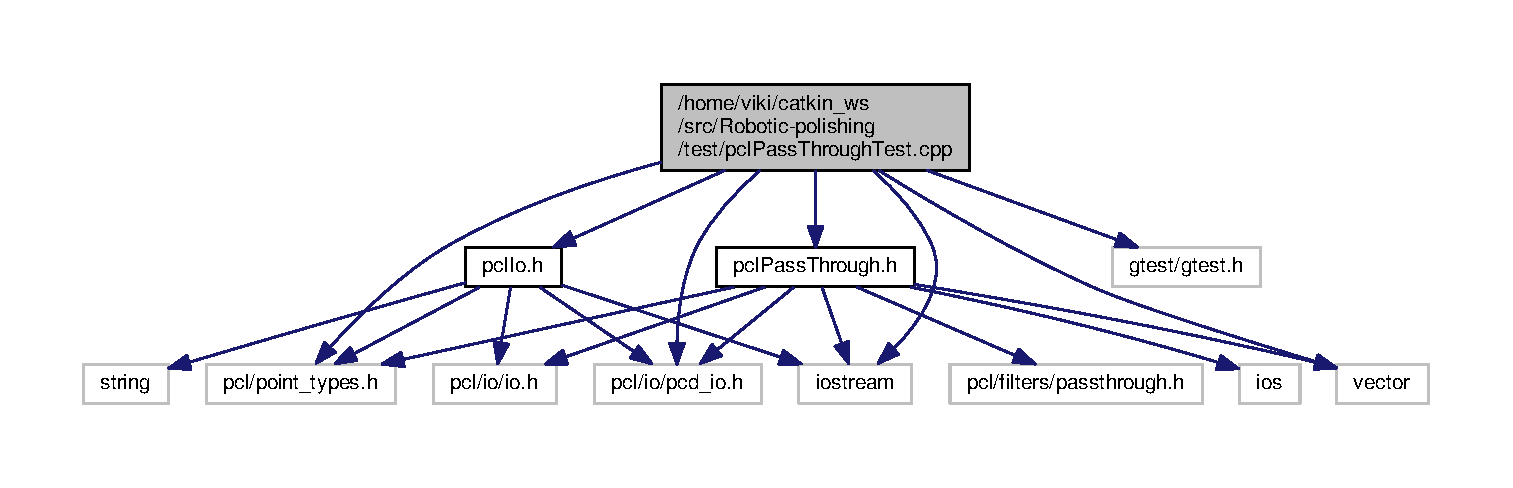
\includegraphics[width=350pt]{pclPassThroughTest_8cpp__incl}
\end{center}
\end{figure}
\subsection*{Functions}
\begin{DoxyCompactItemize}
\item 
\hyperlink{pclPassThroughTest_8cpp_a17ba3ae7544ab54598271bb424069d19}{T\+E\+ST} (pcl\+Pass\+Through\+Test, set\+Limit\+Value)\hypertarget{pclPassThroughTest_8cpp_a17ba3ae7544ab54598271bb424069d19}{}\label{pclPassThroughTest_8cpp_a17ba3ae7544ab54598271bb424069d19}

\begin{DoxyCompactList}\small\item\em \hyperlink{pclPassThroughTest_8cpp_a17ba3ae7544ab54598271bb424069d19}{T\+E\+S\+T(pcl\+Pass\+Through\+Test, set\+Limit\+Value)} will test the set\+Filter\+Xlimit() ,set\+Filter\+Ylimit, set\+Filter\+Zlimit(), and get\+Filter\+Limit() method. \end{DoxyCompactList}\item 
\hyperlink{pclPassThroughTest_8cpp_a3288389cf8648f9cd5967e14765849a1}{T\+E\+ST} (pcl\+Pass\+Through\+Test, Pass\+Through\+Filtered)\hypertarget{pclPassThroughTest_8cpp_a3288389cf8648f9cd5967e14765849a1}{}\label{pclPassThroughTest_8cpp_a3288389cf8648f9cd5967e14765849a1}

\begin{DoxyCompactList}\small\item\em \hyperlink{pclPassThroughTest_8cpp_a3288389cf8648f9cd5967e14765849a1}{T\+E\+S\+T(pcl\+Pass\+Through\+Test, Pass\+Through\+Filtered)} will test the filter\+Process() method. \end{DoxyCompactList}\end{DoxyCompactItemize}


\subsection{Detailed Description}
\hyperlink{pclPassThroughTest_8cpp}{pcl\+Pass\+Through\+Test.\+cpp} consists of 2 unit test cases that test the \hyperlink{classpclPassThrough}{pcl\+Pass\+Through} class. 

\hyperlink{pclPassThroughTest_8cpp_a17ba3ae7544ab54598271bb424069d19}{T\+E\+S\+T(pcl\+Pass\+Through\+Test, set\+Limit\+Value)} will test the set\+Filter\+Xlimit() ,set\+Filter\+Ylimit, set\+Filter\+Zlimit(), and get\+Filter\+Limit() method. \hyperlink{pclPassThroughTest_8cpp_a3288389cf8648f9cd5967e14765849a1}{T\+E\+S\+T(pcl\+Pass\+Through\+Test, Pass\+Through\+Filtered)} will test the filter\+Process() method.

\begin{DoxyAuthor}{Author}
Michael Kam (michael081906) 
\end{DoxyAuthor}
\begin{DoxyRefDesc}{Bug}
\item[\hyperlink{bug__bug000041}{Bug}]No known bugs. \end{DoxyRefDesc}
\begin{DoxyCopyright}{Copyright}
G\+NU Public License. 
\end{DoxyCopyright}

\hypertarget{pclStatisticalOutlierRemovalTest_8cpp}{}\section{/home/viki/catkin\+\_\+ws/src/\+Robotic-\/polishing/test/pcl\+Statistical\+Outlier\+Removal\+Test.cpp File Reference}
\label{pclStatisticalOutlierRemovalTest_8cpp}\index{/home/viki/catkin\+\_\+ws/src/\+Robotic-\/polishing/test/pcl\+Statistical\+Outlier\+Removal\+Test.\+cpp@{/home/viki/catkin\+\_\+ws/src/\+Robotic-\/polishing/test/pcl\+Statistical\+Outlier\+Removal\+Test.\+cpp}}


\hyperlink{pclStatisticalOutlierRemovalTest_8cpp}{pcl\+Statistical\+Outlier\+Removal\+Test.\+cpp} consists of 3 unit test cases that test the pcl\+Statistical\+Outlier\+Removal class.  


{\ttfamily \#include $<$gtest/gtest.\+h$>$}\\*
{\ttfamily \#include $<$pcl/point\+\_\+types.\+h$>$}\\*
{\ttfamily \#include \char`\"{}pcl\+Statistical\+Outlier\+Removal.\+h\char`\"{}}\\*
{\ttfamily \#include $<$iostream$>$}\\*
{\ttfamily \#include $<$vector$>$}\\*
Include dependency graph for pcl\+Statistical\+Outlier\+Removal\+Test.\+cpp\+:
\nopagebreak
\begin{figure}[H]
\begin{center}
\leavevmode
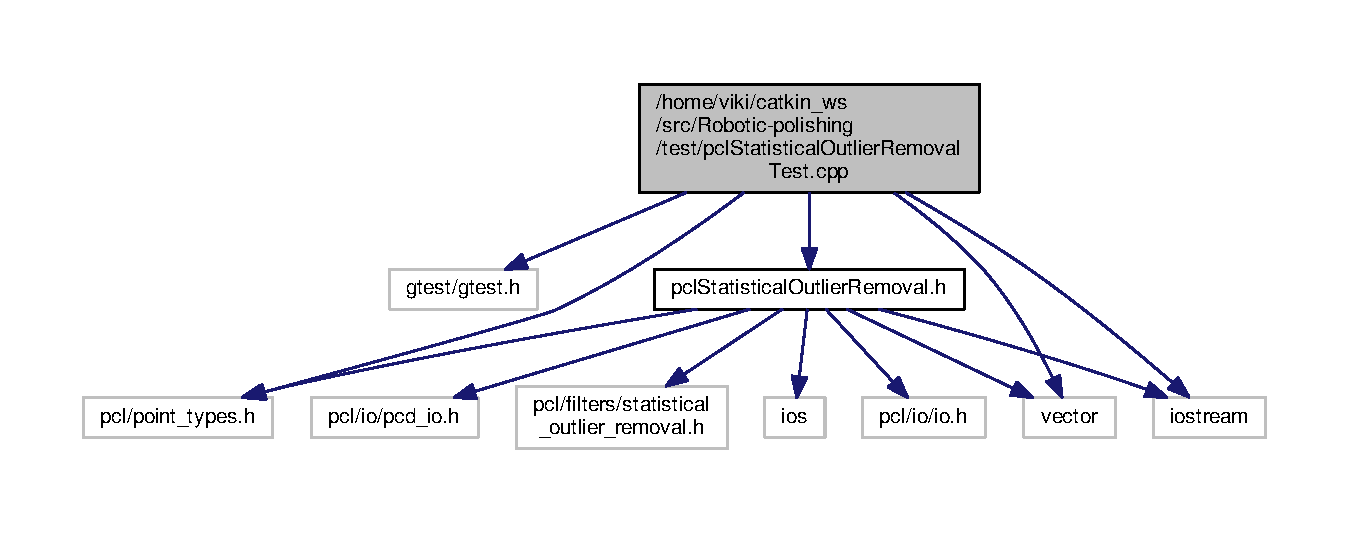
\includegraphics[width=350pt]{pclStatisticalOutlierRemovalTest_8cpp__incl}
\end{center}
\end{figure}
\subsection*{Functions}
\begin{DoxyCompactItemize}
\item 
\hyperlink{pclStatisticalOutlierRemovalTest_8cpp_a7440b4567b31e478a4e0db15713a13df}{T\+E\+ST} (pcl\+Statistical\+Outlier\+Removal\+Test, Set\+Meank\+And\+Thresh)
\item 
\hyperlink{pclStatisticalOutlierRemovalTest_8cpp_ab4412c4c90dfee3682f0cfacb6f02226}{T\+E\+ST} (pcl\+Statistical\+Outlier\+Removal\+Test, Set\+Point\+Cloud)\hypertarget{pclStatisticalOutlierRemovalTest_8cpp_ab4412c4c90dfee3682f0cfacb6f02226}{}\label{pclStatisticalOutlierRemovalTest_8cpp_ab4412c4c90dfee3682f0cfacb6f02226}

\begin{DoxyCompactList}\small\item\em T\+E\+ST(pcl\+Statistical\+Outlier\+Removal\+Test, Set\+Point\+Cloud) will test the get\+Input\+Cloud() and set\+Input\+Cloud() method. \end{DoxyCompactList}\item 
\hyperlink{pclStatisticalOutlierRemovalTest_8cpp_a4bd86cf4614402db58c7e3da6340f15a}{T\+E\+ST} (pcl\+Statistical\+Outlier\+Removal\+Test, S\+O\+R\+Filter\+Test)\hypertarget{pclStatisticalOutlierRemovalTest_8cpp_a4bd86cf4614402db58c7e3da6340f15a}{}\label{pclStatisticalOutlierRemovalTest_8cpp_a4bd86cf4614402db58c7e3da6340f15a}

\begin{DoxyCompactList}\small\item\em \hyperlink{pclStatisticalOutlierRemovalTest_8cpp_a4bd86cf4614402db58c7e3da6340f15a}{T\+E\+S\+T(pcl\+Statistical\+Outlier\+Removal\+Test, S\+O\+R\+Filter\+Test)} will test the filter\+Process() method. \end{DoxyCompactList}\end{DoxyCompactItemize}


\subsection{Detailed Description}
\hyperlink{pclStatisticalOutlierRemovalTest_8cpp}{pcl\+Statistical\+Outlier\+Removal\+Test.\+cpp} consists of 3 unit test cases that test the pcl\+Statistical\+Outlier\+Removal class. 

\hyperlink{pclStatisticalOutlierRemovalTest_8cpp_a7440b4567b31e478a4e0db15713a13df}{T\+E\+S\+T(pcl\+Statistical\+Outlier\+Removal\+Test, Set\+Meank\+And\+Thresh)} will test the get\+Mean\+K(), set\+Stddev\+Mul\+Thresh(), set\+Mean\+K(), and get\+Stddev\+Mul\+Thresh() method. \hyperlink{pclStatisticalOutlierRemovalTest_8cpp_ab4412c4c90dfee3682f0cfacb6f02226}{T\+E\+S\+T(pcl\+Statistical\+Outlier\+Removal\+Test, Set\+Point\+Cloud)} will test the get\+Input\+Cloud() and set\+Input\+Cloud() method. \hyperlink{pclStatisticalOutlierRemovalTest_8cpp_a4bd86cf4614402db58c7e3da6340f15a}{T\+E\+S\+T(pcl\+Statistical\+Outlier\+Removal\+Test, S\+O\+R\+Filter\+Test)} will test the filter\+Process() method.

\begin{DoxyAuthor}{Author}
Michael Kam (michael081906) 
\end{DoxyAuthor}
\begin{DoxyRefDesc}{Bug}
\item[\hyperlink{bug__bug000042}{Bug}]No known bugs. \end{DoxyRefDesc}
\begin{DoxyCopyright}{Copyright}
G\+NU Public License. 
\end{DoxyCopyright}


\subsection{Function Documentation}
\index{pcl\+Statistical\+Outlier\+Removal\+Test.\+cpp@{pcl\+Statistical\+Outlier\+Removal\+Test.\+cpp}!T\+E\+ST@{T\+E\+ST}}
\index{T\+E\+ST@{T\+E\+ST}!pcl\+Statistical\+Outlier\+Removal\+Test.\+cpp@{pcl\+Statistical\+Outlier\+Removal\+Test.\+cpp}}
\subsubsection[{\texorpdfstring{T\+E\+S\+T(pcl\+Statistical\+Outlier\+Removal\+Test, Set\+Meank\+And\+Thresh)}{TEST(pclStatisticalOutlierRemovalTest, SetMeankAndThresh)}}]{\setlength{\rightskip}{0pt plus 5cm}T\+E\+ST (
\begin{DoxyParamCaption}
\item[{pcl\+Statistical\+Outlier\+Removal\+Test}]{, }
\item[{Set\+Meank\+And\+Thresh}]{}
\end{DoxyParamCaption}
)}\hypertarget{pclStatisticalOutlierRemovalTest_8cpp_a7440b4567b31e478a4e0db15713a13df}{}\label{pclStatisticalOutlierRemovalTest_8cpp_a7440b4567b31e478a4e0db15713a13df}
@ brief T\+E\+ST(pcl\+Statistical\+Outlier\+Removal\+Test, Set\+Meank\+And\+Thresh) will test the get\+Mean\+K(), set\+Stddev\+Mul\+Thresh(), set\+Mean\+K(), and get\+Stddev\+Mul\+Thresh() method. 
\hypertarget{pclVoxelTest_8cpp}{}\section{/home/viki/catkin\+\_\+ws/src/\+Robotic-\/polishing/test/pcl\+Voxel\+Test.cpp File Reference}
\label{pclVoxelTest_8cpp}\index{/home/viki/catkin\+\_\+ws/src/\+Robotic-\/polishing/test/pcl\+Voxel\+Test.\+cpp@{/home/viki/catkin\+\_\+ws/src/\+Robotic-\/polishing/test/pcl\+Voxel\+Test.\+cpp}}


\hyperlink{pclVoxelTest_8cpp}{pcl\+Voxel\+Test.\+cpp} consists of 3 unit test cases that test the \hyperlink{classpclVoxel}{pcl\+Voxel} class.  


{\ttfamily \#include \char`\"{}pcl\+Voxel.\+h\char`\"{}}\\*
{\ttfamily \#include \char`\"{}pcl\+Io.\+h\char`\"{}}\\*
{\ttfamily \#include $<$gtest/gtest.\+h$>$}\\*
{\ttfamily \#include $<$pcl/io/pcd\+\_\+io.\+h$>$}\\*
{\ttfamily \#include $<$pcl/point\+\_\+types.\+h$>$}\\*
{\ttfamily \#include $<$iostream$>$}\\*
{\ttfamily \#include $<$vector$>$}\\*
Include dependency graph for pcl\+Voxel\+Test.\+cpp\+:
\nopagebreak
\begin{figure}[H]
\begin{center}
\leavevmode
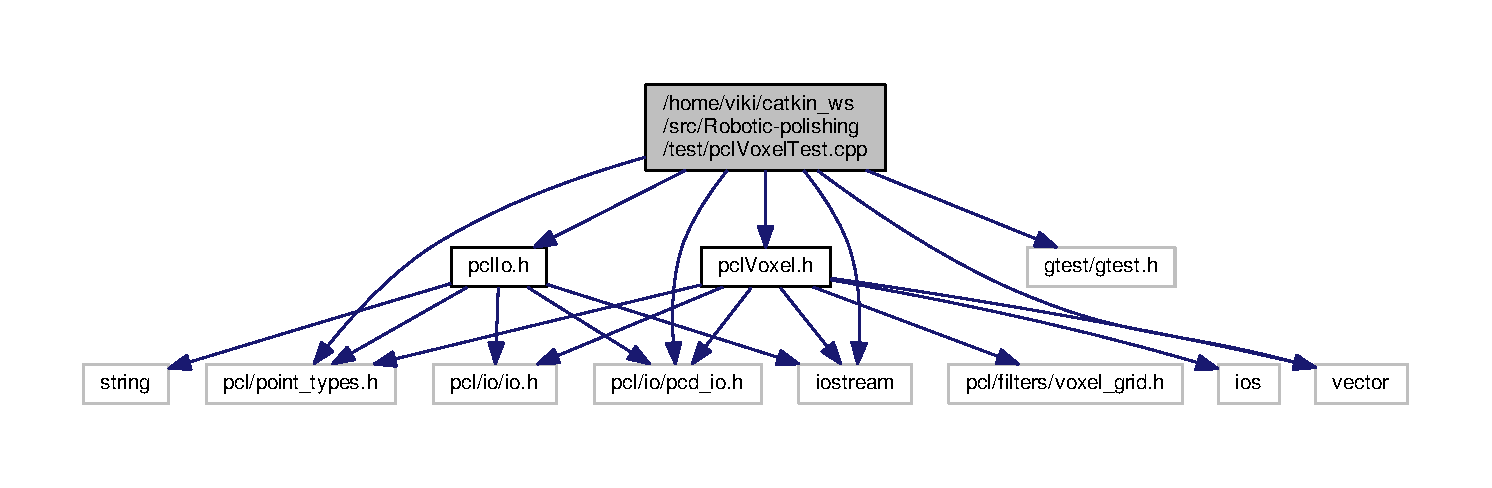
\includegraphics[width=350pt]{pclVoxelTest_8cpp__incl}
\end{center}
\end{figure}
\subsection*{Functions}
\begin{DoxyCompactItemize}
\item 
\hyperlink{pclVoxelTest_8cpp_ab975b9c05d07fcea10cd0d3a9ce5ab3e}{T\+E\+ST} (pcl\+Voxel\+Test, set\+Leaf\+Value)\hypertarget{pclVoxelTest_8cpp_ab975b9c05d07fcea10cd0d3a9ce5ab3e}{}\label{pclVoxelTest_8cpp_ab975b9c05d07fcea10cd0d3a9ce5ab3e}

\begin{DoxyCompactList}\small\item\em \hyperlink{pclVoxelTest_8cpp_ab975b9c05d07fcea10cd0d3a9ce5ab3e}{T\+E\+S\+T(pcl\+Voxel\+Test, set\+Leaf\+Value)} will test the set\+Leaf\+Size() and get\+Leaf\+Size() method. \end{DoxyCompactList}\item 
\hyperlink{pclVoxelTest_8cpp_a8f1ee4768a36f1296e75ac0b7c4b6b3d}{T\+E\+ST} (pcl\+Voxel\+Test, setpcl\+Cloud)\hypertarget{pclVoxelTest_8cpp_a8f1ee4768a36f1296e75ac0b7c4b6b3d}{}\label{pclVoxelTest_8cpp_a8f1ee4768a36f1296e75ac0b7c4b6b3d}

\begin{DoxyCompactList}\small\item\em \hyperlink{pclVoxelTest_8cpp_a8f1ee4768a36f1296e75ac0b7c4b6b3d}{T\+E\+S\+T(pcl\+Voxel\+Test, setpcl\+Cloud)} will test the get\+Input\+Cloud() and set\+Input\+Cloud() method. \end{DoxyCompactList}\end{DoxyCompactItemize}


\subsection{Detailed Description}
\hyperlink{pclVoxelTest_8cpp}{pcl\+Voxel\+Test.\+cpp} consists of 3 unit test cases that test the \hyperlink{classpclVoxel}{pcl\+Voxel} class. 

\hyperlink{pclVoxelTest_8cpp_ab975b9c05d07fcea10cd0d3a9ce5ab3e}{T\+E\+S\+T(pcl\+Voxel\+Test, set\+Leaf\+Value)} will test the set\+Leaf\+Size() and get\+Leaf\+Size() method. T\+E\+S\+T(pcl\+Voxel\+Test, point\+Cloud\+Down\+Sampleing) will test the filter\+Process() method. \hyperlink{pclVoxelTest_8cpp_a8f1ee4768a36f1296e75ac0b7c4b6b3d}{T\+E\+S\+T(pcl\+Voxel\+Test, setpcl\+Cloud)} will test the get\+Input\+Cloud() and set\+Input\+Cloud() method.

\begin{DoxyAuthor}{Author}
Michael Kam (michael081906) 
\end{DoxyAuthor}
\begin{DoxyRefDesc}{Bug}
\item[\hyperlink{bug__bug000043}{Bug}]No known bugs. \end{DoxyRefDesc}
\begin{DoxyCopyright}{Copyright}
G\+NU Public License. 
\end{DoxyCopyright}

%--- End generated contents ---

% Index
\backmatter
\newpage
\phantomsection
\clearemptydoublepage
\addcontentsline{toc}{chapter}{Index}
\printindex

\end{document}
